%
% Master Thesis, Sven Köppel 2014
%
% This text file is encoded as utf-8 and was compiled with
% pdf(la)TeX from the TeX Live 2013/Debian distribution,
% as it is installed at the Ubuntu 14.04 computers
% at FIAS, Goethe-Universität Frankfurt.
%
%
\documentclass[12pt,a4paper]{report}
\usepackage[utf8]{inputenc}
\usepackage[backref=page]{hyperref}
\hypersetup{linktocpage}
%\usepackage[ngerman]{babel}
\usepackage[american]{babel}
\usepackage{amsmath} % xrightarrow, ...
\usepackage{cite}
\usepackage{units} % nicefrac
\usepackage{datetime} % fuer Uhrzeit im \date
\usepackage{wrapfig} % bilder rechts
\usepackage{caption} % fuer subcaption
\usepackage[list=true,listformat=simple]{subcaption} % subfigures with lof listing
\usepackage{graphicx} % Bilder allgemein einbinden
%\usepackage{tabularx} % Tabellen
\usepackage{multirow} % row span
\usepackage{lastpage} % Anzahl Seiten
\usepackage{multicol} % zweispaltige Titelseite
\usepackage{a4wide} % bessere Papiernutzung
\usepackage{fancyhdr} % Header/Footer
\pagestyle{fancy} % Kopf/Fussbereich der Seiten
\usepackage{amssymb} % therefore = dreieckdots
\usepackage{array} % tables
\usepackage{booktabs} % better tables
\usepackage{tabularx} % even better tables
\usepackage{floatrow} % caption beside image
\usepackage[toc]{appendix}
\usepackage[usenames,dvipsnames]{color} % more colors
\usepackage[nottoc,numbib]{tocbibind} % Quellenverzeichnis in TOC
\usepackage{titling} % \thetitle, \theauthor, ...
\usepackage[skins,theorems]{tcolorbox} % Formelboxen
\usepackage[percent]{overpic} % text on pictures
%\usepackage{titlesec} % chapters formatieren
\usepackage{etoolbox} % lof
\usepackage[subnum]{cases} % numbered cases

\usepackage{tikz} % commutative diagrams
\usetikzlibrary{matrix}

% try PDF compression with pdflatex
% actually has no effect.
\pdfminorversion=5 \pdfcompresslevel=9 \pdfobjcompresslevel=3

% to better spot "missing $ inserted" errors
%\usepackage{syntonly}
%\syntaxonly

% Introducing CHAPTERS instead sections
\numberwithin{equation}{chapter}
\usepackage{chngcntr}
\counterwithin{figure}{chapter}

% chapters platzsparender formatieren
%\titleformat{\chapter}{hang}
%  {}{Chapter \thesection}{}{}
%\titlespacing*{\chapter}{0cm}{-\topskip}{0pt}[0pt]
\patchcmd{\chapter}{\thispagestyle{plain}}{}{}{}

% List of figures: no spacing between per-chapter figures in LoF
\makeatletter
% \patchcmd{<cmd>}{<search>}{<replace>}{<succes>}{<failure>}
%\def\@gobblesix#1#2#3#4#5#6{}
%\patchcmd{\@chapter}% <cmd>
%  {\chaptermark{#1}}% <search>
%  {\chaptermark{#1}\@gobblesix}% <replace>
%  {}{}% <success><failure>
%\makeatother

% noch ein Versuch, klappt einfach nicht!!
\makeatletter
\patchcmd{\@chapter}{%
        \addtocontents{lof}{\addvspace{10\p@}}%
        %\addtocontents{lot}{\addvspace{10\p@}}%
}{}{\message{Could patch chapter}}{\message{Failed to patch \string\@chapter}}
\makeatother
  
% Tiny chapters that look like sections
% (top sections in article layout)
\newcommand{\tinychapter}[1]{%
\addtocounter{chapter}{1}%
\setcounter{section}{0}% ja das ist be***
\setcounter{subsection}{0}%
\addcontentsline{toc}{chapter}{\protect\numberline{\thechapter} #1}
\section*{\thechapter\quad{} #1}}
 
% Und passend dazu das... richtig, tinysection,
% welches eine subsection "simuliert", also so aussieht
% wie subsection. Wär das nicht alles schön, wenn Latex
% CSS könnte!
\newcommand{\tinysection}[1]{%
\addtocounter{section}{1}%
\setcounter{subsection}{0}%
\addcontentsline{toc}{section}{\protect\numberline{\thesection} #1}
\subsection*{\thesection\quad{} #1}}


% abgefahrenes highlighting von formeln
\usepackage{xcolor}
% klappt net, was einfacheres:
\newcommand{\highlight}[1]{%
  \colorbox{green!30}{$\displaystyle#1$}}
  
% colored boxes for things todo
% Alternative dazu (gut fuer Seitenanmerkungen):
% http://tex.stackexchange.com/a/73418/49958
\usepackage[draft,colorinlistoftodos,shadow,textsize=small]{todonotes}   % notes showed
\presetkeys{todonotes}{noline}{}

% alternative, used before:
\usepackage{mdframed}
\mdfdefinestyle{todo}{
	linecolor=red,
	backgroundcolor=yellow!40,
	linewidth=5pt,
	topline=false,
	rightline=false,
	bottomline=false
}
% definiere \begin{todo} und \todo{blabla} auf einmal:
\usepackage{environ}
\NewEnviron{todoBlock}%[1]
  {\begin{mdframed}[style=todo]
  	 \BODY
   \end{mdframed}}
   
% double equations next to each other
% http://tex.stackexchange.com/questions/120670/equations-side-by-side-both-numbers-on-the-right
\NewEnviron{double}[2]
  {\begin{equation*}
     \refstepcounter{equation}\latexlabel{#1}
     \refstepcounter{equation}\latexlabel{#2}
     \BODY % write something like a=b\qquad c=d
     \tag{\ref*{#1}, \ref*{#2}}
   \end{equation*}}
\AtBeginDocument{\let\latexlabel\label}   

% Revisited environment
\NewEnviron{revisited}[1]
  {\begin{equation} \tag{\ref{#1} revisited}
   \BODY % This shall be a complete copy
   \end{equation}}
   

% Kopfzeile/Fusszeile mit fancy
\fancyhead{}
%\fancyhead[L]{\thesection}
\fancyfoot{}
%\fancyfoot[FL]{\textcolor{gray}{\thedate}}
% während Entwicklung war das hier die Fußnote.
%\fancyfoot[FR]{\thepage {} / \pageref*{LastPage}}
\fancyfoot[FR]{\thepage}
\renewcommand{\headrulewidth}{0 pt}

% Remove Appendix extra page (only with text "Appendices")
%\renewcommand{\appendixpage}{}
% - just remove it by leaving out "page" in appendix package options.


% Farben (werden derzeit nur in hypersetup verwendet)
\usepackage{color}
\definecolor{darkblue}{rgb}{0,0,.6}
\definecolor{darkred}{rgb}{.1,0,0}
\definecolor{darkgreen}{rgb}{0,.5,0}

% Schriften
% Palatino for rm and math | Helvetica for ss | Courier for tt

% Linux Libertine, neue Schrift, vgl
% http://tex.stackexchange.com/questions/9533/what-best-combination-of-fonts-for-serif-sans-and-mono-do-you-recommend
\usepackage{libertine}

%\usepackage{mathpazo} % math & rm
%\linespread{1.05}        % Palatino needs more leading (space between lines)
%\usepackage[scaled]{helvet} % ss
\usepackage{inconsolata} % tt
\normalfont
\usepackage[T1]{fontenc}

% Common Keywords
\title{Ultraviolet improved black holes}
\def\thesubtitle{Master Thesis}
\author{Sven Köppel}
\date{\today, \currenttime}
\def\thekeywords{
    abc, def, ghi % wird nicht genutzt, s.u. pdfkeywords.
    }

% Hyperref aufsetzen
\hypersetup{
    pdftitle={\thetitle - \thesubtitle},
    pdfauthor={\theauthor},
    pdfsubject={master thesis},
    pdfkeywords={physik} {master} {thesis} {uni} {frankfurt} {fias} {itp} {quantum gravity} {black holes},
    colorlinks=true,        % test: stat gerahmten Links
    linkcolor=red,          % color of internal links
    citecolor=darkgreen,    % color of links to bibliography
    filecolor=darkred,      % color of file links
    urlcolor=cyan,          % color of external links
    bookmarks=true          % show the toc
}

% Bibliography
% war: ieeetr
% jetzt: Living Reviews, Vorteil: DOI und ArxiV-Verlinkung, Backlinks.
% http://blog.relativity.livingreviews.org/author-information/citation-guidelines/#bibtex
\bibliographystyle{livrevrel}


% Backrereferences in Bibliography,
% http://tex.stackexchange.com/questions/15971/bibliography-with-page-numbers
\renewcommand*{\backref}[1]{}
\renewcommand*{\backrefalt}[4]{%
    \ifcase #1 (Not cited.)%
    \or        (Cited on page~#2.)%
    \else      (Cited on pages~#2.)%
    \fi}

\begin{document}

\thispagestyle{empty}
   \begin{center}
   	% dezente Schattierung
    \Huge \textcolor{black!90}{\textbf{\thetitle}} \\
    \vspace{.5cm}
    \LARGE \textcolor{black!80}{\textbf{\thesubtitle}} \\
    \Large
   	\vspace{.9cm}
    \textsc{\theauthor} \\
    \vspace{.9cm} 
    	December 2014 \\
    \vspace{1.5cm}
    % for the list of figures :D
    \addcontentsline{lof}{figure}{3d embedding diagram without axis of the deSitter self-regular black hole}%
    
    %http://mathematica.stackexchange.com/questions/57434/plotting-semi-hollow-spheres
    \includegraphics[width=9.5cm]{figures/titlepage-3d.png} \\
    \vfill{}
    \large
    \vspace{1.5cm}
    \begin{tabular}{@{}>{\itshape}rl@{}}
	  First Supervisor: & \textsc{PD Dr. Piero Nicolini} \\[1ex]
	  Second Supervisor: & \textsc{Prof. Dr. Marcus Bleicher}
    \end{tabular}
    \\
    \vspace{1cm}
    \Large
    \textcolor{black!70}{
    \textsc{Institute for Theoretical Physics \&} \\
    \textsc{Frankfurt Institute for Advanced Studies} \\
    }%endofcolor
    \vspace{2cm}
    \includegraphics[width=4.9cm]{figures/goethe-logo.pdf}
    %\\
    %\vspace{1cm}
    %\large
    %\colorbox{red!40}{Vorliegende Version ist vom {\bf \thedate}}
	\end{center}

\newpage
% 2. Seite: Zweites Deckblatt
% Abstract, statt \begin{abstract} nutze
\begin{center}
 {\bfseries Abstract\vspace{-.5em}\vspace{0pt}}
\end{center}

In this thesis, Planck size black holes are discussed.
Specifically, new families of black holes are presented. Such black holes
exhibit an improved short scale behaviour and can be used to implement
gravity self-complete paradigm.
Such geometries are also studied within the ADD large extra-dimensional
scenario. This allows black hole remnant masses to reach the TeV scale.
It is shown that the evaporation endpoint for this class of black holes
is a cold stable remnant. One family of black holes considered in this
thesis features a regular de Sitter core that counters gravitational
collapse with a quantum outward pressure.
The other family of black holes turns out to nicely fit into the holographic
information bound on black holes, and lead to black hole area quantization
and applications in the gravitational entropic force. As a result,
gravity can be derived as emergent phenomenon from thermodynamics.

The thesis contains an overview about recent quantum gravity black hole
approaches and concludes with the derivation of nonlocal operators
that modify the Einstein equations to ultra-violet complete field equations.
% \end{abstract}

\vfill

%
%\noindent
%{\bf Master thesis}
%\vspace*{.4cm}
%
%\noindent
%\emph{written at}
%\vspace*{.3cm}
%
%\noindent
%{\bf Institut für theoretische Physik} \\
%Fachbereich Physik \\
%Goethe-Universität Frankfurt am Main \\
%Max-von-Laue-Straße 1 \\
%60438 Frankfurt am Main
%\vspace*{.3cm}
%
%\noindent
%\emph{and}
%\vspace*{.3cm}
%
%\noindent
%{\bf Frankfurt Institute for Advanced Studies (FIAS)} \\
%Ruth-Moufang-Straße 1 \\
%60438 Frankfurt am Main
%
%\vspace{3cm}
\vfill

% About the front page figure
\noindent
{\bf About the front picture} \\

\noindent
\begin{minipage}{0.6\textwidth}
This picture shows an embedding diagram for the self-regular black hole in the outstanding case $\alpha\to\infty$.

By intention, there are no units as this is purely illustrative. The 3d picture can be constructed by rotating the graphs shown on the right around its $y$ axis. The color transition indicates
the position of the black hole event horizon.

For more information about the computation of embedding diagrams, see appendix \ref{sec:embedding-diag}.

%This picture visualizes a kind of black hole proposed in this thesis, compared with the classical Schwarzschild black hole (the well known ``cone''). The red disk indicates the position of the event horizon: Anything ``inside'' the disk cannot get out of it.
%
%More strictly, the 3-dimensional illustration shows an embedding of the equitorial plane of the equitorial plane of the self-regular black hole which gravitational potential is e.g. shown in figure \ref{fig:g00-alpha-inf} for $\alpha\to \infty$. For the sake of better understanding, there is a cut-out to view the inside of the object. The picture can be constructed by rotating the graph shown on the right around it's $y$ axis.
\end{minipage}%
\hspace{.3cm}
\begin{minipage}{0.4\textwidth}
\includegraphics[scale=1]{figures/titlepage-explain.pdf}
\end{minipage}
%
% for the list of figures
\addcontentsline{lof}{figure}{1d embedding diagram $z(r)$ that resembles the 3d title page plot}%


\newpage 
% abkuerzungen:
\renewcommand{\d}{\mathrm{d}}
\newcommand{\dd}[2]{\frac{\mathrm{d} #1}{\mathrm{d} #2}}
\newcommand{\pp}[2]{\frac{\partial #1}{\partial #2}}
\renewcommand{\L}{L_P}
\newcommand{\pr}{p_r}
\newcommand{\psenk}{p_\perp}
\newcommand{\ebenso}{\biggl( ~ \therefore ~ \biggr) }
\newcommand{\metrik}[1]{\d s^2 = \left( #1 \right) \d t^2 \left( #1 \right)^{-1} \d r^2 + r^2 \d \Omega_{D-2}^2 }
\newcommand{\winkel}{r^2 \d \Omega^2}
\newcommand{\dann}{$\rightarrow~$}
\newcommand{\CA}{ {\cal A}}
\newcommand{\C}[1]{ {\cal #1}}
\newcommand{\mn}{_{\mu\nu}}
%\newcommand{\bv}[1]{ \mathbf{ #1 } } % bold vector
% Test:
\newcommand{\bv}[1]{ \boldsymbol{ #1 } } % bold vector
\newcommand{\diag}{\operatorname{diag}}
\newcommand{\res}{\operatornamewithlimits{Res}}
\newcommand{\Res}{\operatornamewithlimits{Res}} % ...
\newcommand{\sign}{\operatorname{sign}}
\newcommand{\musteq}{\stackrel{!}{=}} % must be equal

\renewcommand{\Re}{\mathop{Re}}
\renewcommand{\Im}{\mathop{Im}}

\newcommand{\setN}{\mathbb{N}}
\newcommand{\setR}{\mathbb{R}}
\newcommand{\setC}{\mathbb{C}}


% colored symbols:
% http://tex.stackexchange.com/questions/85033/colored-symbols
\newcommand*{\mathcolor}{}
\def\mathcolor#1#{\mathcoloraux{#1}}
\newcommand*{\mathcoloraux}[3]{%
  \protect\leavevmode
  \begingroup
    \color#1{#2}#3%
  \endgroup
}
% In Text: $a\textcolor{red}{\ast}b$
% In Math: $a\mathcolor{red}{\ast}b$
\newcommand{\redmin}{\mathcolor{red}{-}}
\newcommand{\redplus}{\mathcolor{red}{+}}
\newcommand{\pn}{\mathcolor{OliveGreen}{+ n}}
\newcommand{\n}{ {\mathcolor{OliveGreen}{n}} }

\tableofcontents

\vfill


% Mini fix for todo list section, see 1.6.9. of
% todonotes.pdf documentation
%%% removed for article -> report!!
%\makeatletter\let\chapter\@undefined\makeatother

%\listoftodos

\newpage
%\tinychapter{Introducion}
%\addcontentsline{toc}{section}{Introduction}
%\section*{Introduction}
\chapter{Introduction}
\section{Motivation}
This work is about the quest of contemporary physics on the
smallest scales and biggest energies. By historical
evolution, in the 20th century two opposing theories developed:
For phenomena on the smallest scales (e.g. the constituents of an atom),
quantum physics evolved.
On the other hand, for phenomena on the biggest scales (e.g. the Universe),
general relativity was formulated. 

Combining these two worlds is a big quest in physics. A theory which describes
effects from both the quantum and the gravitational world is a
{\it quantum gravity} theory.

\begin{figure}[h!]
\floatbox[\capbeside\thisfloatsetup{floatwidth=\textwidth,capbesidewidth=sidefil,capbesideposition={right,top}}]{figure}[\FBwidth]{%
\caption[Illustration \emph{cube of physics} taken from \cite{penroseBook}]{The \emph{cube of physics}, a popular illustration
about characteristic constants that describe the regime for
physical phenomena. First appeared in a 1999 book from Roger Penrose~\cite{penroseBook}.

The whirly lines shall encode how hard the author percieved the challenge to find
or handle the theories the arrows point to. Appearently, Penrose finds a theory of
quantum gravity hard to find.
}\label{fig:physics-theory-cube}
}{% floatbox figure:
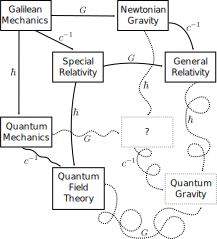
\includegraphics[width=8.0cm]{figures/cube-of-physics-penrose.pdf}
%
% Links therein for Hossenfelder:
% http://backreaction.blogspot.de/2011/05/cube-of-physical-theories.html
% http://svenk.ufopixel.de/tmp/IMG-20130330-WA0001.jpg (BUCH?)
% zB The Natural Laws of the Universe: Understanding Fundamental Constants.  By Jean-Philippe Uzan, Bénédicte Leclercq
}% end of floatbox
\end{figure}

The combination of quantum mechanics and special relativity leads to quantum field theory (QFT) and the formulation of the standard model of particle physics which is exceptionally and unexpectedly successful. From the viewpoint of an high-energy physicist, three of the four fundamental interactions, namely the electromagnetic, weak and strong interactions can be joined into a unified theory, while gravity is simply the weakest and last interaction left as an ``ordinary'' classic field theory. A unification of the three standard model interactions is called grand unified theory (GUT). On the other hand, from the viewpoint of a relativist, general relativity taught us that there is no background space where physics ``takes place''. This new principle leads to a bunch of new physics, where the most remarkable fact is perhaps the existence of black holes as regions of no escape in spacetime or even the existence of wormholes (Einstein-Rosen bridge). Certainly, general relativity had the biggest impact on the science fiction genre.

Physics beyond the Standard Model is an uncomfortable job,
because it still lacks experimental accessibility.
One thing theorists can do is quantum field theory in curved space (QFTCS), the
semiclassical approximation to quantum gravity where quantum fields interact with a
classical background spacetime. In the \emph{cube of physical theories}, as shown
in figure \ref{fig:physics-theory-cube}, QFTCS is ``one step'' from QFT to quantum gravity, because
1-loop graviton contributions are included in the quantum energy momentum tensor at the right hand side of Einstein Field Equations.


Actually, QFTCS opened the door for the first quantum mechanical treatments of strong gravity objects, namely black holes. In the 1970s, this led to the Hawking's groundbreaking prediction of thermal radiation of Schwarzschild black holes. In terms of ``theories'', Hawking radiation is really interdisciplinary:
%
\begin{equation*}
T_\mathrm{H} = \frac{\hbar\ c^3}{8\pi\,G\,M k_\mathrm{B}}
\end{equation*}
%
There are ``ingredients'' from quantum mechanics (Planck constant $\hbar$), Special Relativity (speed of light $c$), Gravitation (Newton's constant $G$) and Thermodynamics (Boltzmann constant $k_B$).

But Hawking's temperature also spots one of the inconsistencies of general relativity: The temperature increases with decreasing mass $M$. As radiating black holes lose mass, they get hotter and hotter. At some point, the validity of QFTCS breaks down. The need for a better theory arises.

\section{The problems and the approach}
The breakdown of QFTCS is one of the problems addressed in this thesis. Other problems are
\begin{itemize}
\item The curvature singularity in the center of the Schwarzschild black hole, discussed in section \ref{sec:exact-sols}.
\item The hierarchy problem in the Standard model, discussed in section \ref{sec:extra-dimensions}.
\item The black hole--particle duality at high energies, where quantum mechanics and General Realtivity predict different length scales, discussed in section \ref{sec:bh-particle-duality}.
\end{itemize}
Black hole geometries with an improved short scale behaviour are proposed. They are based on the self-complete paradigm of gravity. These modified geometries engage all three problems outlined above.

\section{Outline}
Chapter \ref{sec:GR} is an introductory section about general relativity. It will give an introduction to the formalism and shortly derive the Einstein equation. Then the first solutions on GR are shown and the different types of singularities and their origins are discussed.  The large spatial extra dimension scenario is outlined.

Chapter \ref{sec:minial-length} is devoted to the minimal length in physics. The particle--black hole duality is discussed and nonlocal gravity formalism is proposed. The generalized uncertainty principle is given as an example for minimal length physics.

In chapter \ref{sec:generic-H}, the formalism for a class of short-scale modified static isotropic black holes in higher dimensions is prepared. To do so, Einstein Equations are solved for an ideal static isotropic ``blurred'' matter ball that shall describe a ``quasi-classical'' mass point. Thermodynamical properties like temperature, heat capacity and entropy are derived and a nonlocal operator is determined in terms of a Fourier transform.

Chapter \ref{sec:holo} and \ref{sec:self-regular} are devoted to two classes of black holes that are based on the more generic class discussed in chapter \ref{sec:generic-H}. In these two chapters, physical properties and implications are discussed based on the formalism introduced before.


\chapter{Theoretical background}\label{sec:GR}


\section{General Relativity}
In this section, a short derivation of general relativity (GR) is given. It is the geometrical theory of gravitational interaction from matter and the major framework used in this work. To do so, some core concepts of differential geometry on manifolds are retraced briefly in order to derive the einstein field equations (EFE) by Hamiltonian's principle of least action. Exact definitions of the new vector concept are skipped in favour of condensing the ideas. In this text I follow the notations of \cite{WaldGR,MTW,carroll,kochPhd,WaldTeaching}. They prefer abstract index notation as a more fundamental approach to introduce Riemannian geometry. In contrast, some tensors may also be derived by ``index constraints'' as done in \cite{fliessbach}. This is less elegant but more straightforward.


\subsection{Differential Geometry}
In curved space geometry, intuition about well-known mathematical symbols like vectors as ``position vectors'' fails \cite{WaldTeaching}. The mathematical approach is a differential description using the fact that manifolds $M$ are locally flat (they look ``nearly'' flat). Thus the tangent vector $V$ is introduced as a directional derivative operator. The components of such a vector may be denoted as
\begin{equation}
V(f) = V^\mu \pp{f}{x^\mu}.
\end{equation}
The vector $V$ maps functions $f \in C^\infty(M,\setR)$ to $\setR$. With a fixed point $p\in M$, it defines the tangent vector space $V_p$. Introducing the dual space $V_p^*$ and the dual dual space $V_p^{**} \cong V_p$ yields to the definition of tensors as a multilinear mappings from vectors and dual vectors into numbers \cite{WaldGR}.

\subsection{Covariant Derivation Operator}
As for two points $p,q \in M$, the tangent spaces $V_p$ and $V_q$ can not directly be compared. For example, defining for the vector $V^\mu$ a traditional derivative (cf. \cite[page 208]{MTW})
\begin{equation}\label{eq:GR-deriv-wrong}
\pp{V^\mu}{x^\nu} =
\lim_{h\to 0}
\frac{V^\mu(x^1,\dots,x^\nu + h^\nu,\dots,x^n)
- V^\mu(x^1,\dots,x^\nu + h^\nu,\dots,x^n)}{h^\nu}
\end{equation} 
fails as even $x$ and $x+h$ may not be compared directly. As a solution, a covariant derivation operator $\nabla$ by means of the parallel transport is derived. This operator will transform like a tensor.
%\todo{{\bf PN:} Was heißt "compared"? Klären.}

While Wald \cite[page 31]{WaldGR} designates requirements for the covariant derivation (linearity, Leibnitz rule, index contraction commutativity, consistency with the index free notation and vanishing torsion tensor/commutativity) and derives the existence of a \emph{connection coefficient} $\Gamma^a_{bc}$, one can also introduce the connection coefficient as the link in the parallel transport which shall be the ``correct'' way to denote the derivative \eqref{eq:GR-deriv-wrong}:%, as done in \cite{kochPhd}: - und \cite{MTW}
\begin{equation}\label{eq:GR-connection-coefficient}
V^\mu(x \to x+h) := V^\mu(x) - V^\lambda(x)
\Gamma^\mu_{\nu\lambda} h^\nu.
\end{equation}
By replacing the traditional difference $V^\mu(x)-V^\mu(x+h)$ by $V^\mu(x) - V^\mu(x\to x+h)$ in equation \eqref{eq:GR-deriv-wrong}, one immediately ends up with the definition of the covariant derivative
\begin{equation}
\nabla_\mu V^\nu = \partial_\mu V^\nu + \Gamma^\nu_{\mu\sigma} V^\sigma.
\end{equation}
The covariant derivative naturally extends when computing derivatives of tensors of arbitrary rank. %While a mathematical rigorous proof requires a lot of additional notation, I will sketch the concept in favour to derive the special case derivatives of tensors of rank (2,0), (1,1) and (0,2) which are frequently used in the subsequent sections.
For a $(k,l)$ tensor $T$ the derivative is given (without proof) by
\begin{equation}
\nabla_\alpha
T^{\lambda_1 \dots \lambda_k}_{\mu_1 \dots \mu_l}
=
\partial_\alpha T^{\lambda_1 \dots \lambda_k}_{\mu_1 \dots \mu_l}
+
\sum_{i=1}^k
\Gamma^{\lambda_i}_{\alpha \beta}
T^{\lambda_1 \dots \beta \dots \lambda_k}_{\mu_1 \dots \mu_l}
-
\sum_{j=1}^l
\Gamma^{\beta}_{\alpha \mu_i}
T^{\lambda_1 \dots \lambda_k}_{\mu_1 \dots \beta \dots \mu_l}.
\end{equation}
The indices $\lambda_1\dots\beta\dots\lambda_k$ have to be read in a way that $\beta$ replaces the index variable at that place. For example, the covariant derivative of a $(2,2)$ tensor reads
\begin{equation}
\nabla_\alpha T^{\lambda\delta}_{\mu\nu}
= \partial_\alpha T^{\lambda\delta}_{\mu\nu}
+ \Gamma^\lambda_{\alpha\beta} T^{\beta\delta}_{\mu\nu}
+ \Gamma^\delta_{\alpha\beta} T^{\lambda\beta}_{\mu\nu}
- \Gamma^\beta_{\alpha\mu} T^{\lambda\delta}_{\beta\nu}
- \Gamma^\beta_{\alpha\nu} T^{\lambda\delta}_{\mu\beta}.
\end{equation}

\subsection{The Metric}
The connection symbol $\Gamma^\alpha_{\beta\gamma}$ introduced in equation \eqref{eq:GR-connection-coefficient} is still ambigous. As soon as one equippes the manifold with a metric $g_{\mu\nu}$, there is a special choice, constrained by the requirement that scalars shall be invariant under parallel transport (in colloquial terms, scalars are required to be the same in any coordinate system). The inner product of two arbitrary vectors $\boldsymbol{v}$ and $\boldsymbol{w}$ is a scalar and shall therefore also be invariant under any parallel transport $t^\alpha \nabla_\alpha$. This leads to
%\todo{{\bf PN} will Gl. \eqref{eq:metric-compat} vorgerechnet bekommen. Nachschauen wie die Argumentation ging.}
\begin{equation} \label{eq:metric-compat}
0 \stackrel != t^\alpha \nabla_\alpha g_{\beta\gamma} v^\beta w^\gamma
\quad\Rightarrow\quad 0 = \nabla_\alpha g_{\beta\gamma}.
\end{equation}
A connection $\Gamma_{\alpha\beta}^\gamma$ is called \emph{metric compatible} if it fulfills \eqref{eq:metric-compat} and is torsion-free ($\Gamma_{\alpha\beta}^\gamma = \Gamma_{(\alpha\beta)}^\gamma$, with $\Gamma_{(\alpha\beta)}$ being the symmetric part of $\bv \Gamma$ according to eq. \eqref{eq:formulary-symmetric-part}. See e.g. \cite[page 99]{carroll} for torsion).

These uniquely determined connection symbols are called \emph{Christoffel symbols}. They allow for computing the parallel transport and the covariant derivative from the metric:
\begin{equation}
\Gamma^\delta_{\alpha\beta} = \frac{1}{2}
g^{\delta \gamma}
(\partial_\alpha g_{\beta \delta}
+ \partial_\beta g_{\alpha \delta}
+ \partial_\gamma g_{\alpha \beta}
).
\end{equation}

\subsection{Curvature}

\begin{figure}[b!]
\floatbox[\capbeside\thisfloatsetup{floatwidth=\textwidth,capbesidewidth=sidefil,capbesideposition={right,top}}]{figure}[\FBwidth]{%
\caption[Illustration for closed loops in Riemann geometry]{Illustration of the closed loop parallel transport on infinitesimal linear displacements $\Delta_i^\mu$. When performing the calculation in equation \ref{eq:GR-sys-curvature}, on curved spacetimes one finds a defect which defines the Riemann tensor. This means that the vector at the beginning (point $a$) does not match the vector after the loop any more.
}\label{fig:parallel-transport}}{% turn grid on: 	scale=1,grid,tics=10
\begin{overpic}[width=7.5cm,unit=1mm]{figures/parallel-transport.pdf}
% coordinates: (left,bottom) scaling from 0-100.
 \put (26,24) {$a$}
 \put (50,23) {$\Delta_1$}
 \put (71,24) {$b$}
 \put (73,35) {$\Delta_2$}
 \put (75,52) {$c$}
 \put (57,53) {$-\Delta_1$}
 \put (33,52) {$d$}
 \put (20,40) {$-\Delta_2$}
\end{overpic}}
\end{figure}


It is important to remember that for a manifold $M$ there exist different choices of coordinate systems, and only if one founds flat space coordinates that are applicable everywhere (that is, ${\bv \Gamma}=0$ for all $p\in M$), the manifold is not curved. This reasoning does not work the other way, as the example of choosing polar coordinates $(t,r,\phi,\theta)$ in flat space shows: Some entries are non-zero (e.g. $\Gamma^\phi_{r\phi}=1/r$), but the space is still flat.

In favour to get a measure for spacetime curvature, one can analyse the ``defects'' of parallel transport around a closed loop with infinitesimal extend. It will be shown that the change is described by a $(1,3)$-curvature tensor  called \emph{Riemann curvature tensor}.

In the present setup (cf. figure \ref{fig:parallel-transport}), the vector $V^\mu$ is moved around the closed path $a\to b\to c\to d$ with infinitesimal spacings $+\Delta_1^\mu, +\Delta_2^\mu, -\Delta_1^\mu, -\Delta_2^\mu$. One can determine the missing part $\#$ when coming back to $a$ by explicit computation of the vector $V^\mu$ at the space time points:
\begin{subequations}\label{eq:GR-sys-curvature}
\begin{alignat}{3}
V^\mu(a) &= V^\mu(a) \\
\label{eq:GR-sys-curvature1}
V^\mu(b)
&= V^\mu(a \to a + \Delta_1)
&&= V^\mu(a) - V^\alpha(a) \Gamma^\mu_{\beta \alpha}(a) \Delta_1^\beta \\
\label{eq:GR-sys-curvature2}
V^\mu(c)
&= V^\mu(b \to b + \Delta_2)
&&= V^\mu(b) - V^\gamma(b) \Gamma^\mu_{\delta \gamma}(b) \Delta_2^\delta \\
V^\mu(d)
&= V^\mu(c \to c - \Delta_1)
&&= V^\mu(c) - V^\epsilon(c) \Gamma^\mu_{\kappa \epsilon}(c) (-\Delta_1^\kappa) \\
\# V^\mu(a)
&= V^\mu(d \to d - \Delta_2)
&&= V^\mu(d) - V^\lambda(d) \Gamma^\mu_{\omega \lambda}(d) (-\Delta_2^\omega)
\end{alignat}
\end{subequations}
Recursively inserting all equations into each other gives a long expression where all linear terms $\C O(\Delta_i^\nu)$ vanish. All third powers $\C O(\Delta_i^\nu \Delta_j^\xi \Delta_k^\rho)$ are ignored, so the result is proportional to second order terms $\C O(\Delta^\gamma_1 \Delta^\delta_2)$ after appropriate index relabeling. Note that the Christoffel symbols (also) depend on the point where they are evaluated at. They can be simply moved e.g. at the first insertion step \ref{eq:GR-sys-curvature1} into \ref{eq:GR-sys-curvature2} by $\Gamma(b) = \Gamma(a) + \partial_\nu \Delta_1^\nu \Gamma(a)$. One ends up with the definition of the Riemann tensor $R^\mu_{\alpha\beta\gamma}$ as a piece of the missing part
\begin{equation}
\# V^\mu(a) =
V^\mu(a)
\Big( \underbrace{
\partial_\beta \Gamma^\mu_{\gamma\alpha}
- \partial_\gamma \Gamma^\mu_{\beta\alpha}
+ \Gamma^\delta_{\gamma\alpha} \Gamma^\mu_{\beta\delta}
- \Gamma^\delta_{\beta\alpha} \Gamma^\mu_{\gamma\delta}
}_{R^\mu_{\alpha\beta\gamma}} \Big)
\Delta_1^\gamma \Delta_2^\delta.
\end{equation}

By tensor contraction, one can define the Ricci tensor $R_{\mu\nu} = R^\lambda_{\mu\lambda\nu}$ and finally the Ricci scalar $R=R^\lambda_\lambda$. This quantity is also called scalar curvature and it is the simplest invariant that gives information about flatness of space: As soon as $R=0$ everywhere, the space is flat.

Most significance for the next section has the Einstein curvature tensor $\bv G$, defined by a linear combination of the Ricci tensor and the curvature scalar as
\begin{equation}
G_{\mu\nu} = R_{\mu\nu}+ \frac{1}{2} g_{\mu\nu} R.
\end{equation}

\subsection{Einstein field equations}\label{sec:deriving-efe}
Einstein field equations (or shorter: Einstein's equations) can be derived from a variational principle (Hamliton principle $\delta S=0$ on the action $S$). They can also be derived by other means, e.g. symmetry aspects leaving only one choice for combining $G_{\mu\nu}$ and the energy density tensor $T_{\mu\nu}$. 
%
%With the \emph{Strong principle of equivalence} and the \emph{principle of general covariance} as ingredients, we will derive Einstein equations from a variational principle on the Action $\delta S = 0$ (Hamiltonian principle). Other forms of deriving the 
%
% Actually, there exist a bunch of other derivations, which e.g derive the Einstein tensor $G_{\mu\nu}$ seperately, with the Ansatz $G_{\mu\nu} = \kappa T_{\mu\nu}$.

Here, the ansatz will be the action $S$, defined by the Lagrangian $\C L = \C L_G + \C L_M$, that is, the gravitational part and the matter part. In terms of field theory, interactions are intermediated by $\C L_G$, while $\C L_M$ contains the source terms. Those two parts are guessed: Here we take basically taking the curvature scalar $R$ and the trace of the energy density tensor $T=T^\lambda_\lambda$. The low energy matching is traditionally accomplished by a prefactor $\kappa$, so one ends up with the \emph{Einstein-Hilbert action} including matter,
\begin{equation}\label{eq:Einstein-Hilbert-action}
S = \int \sqrt{-g}~\d^4 x \left(\frac{R}{2\kappa} + T\right).
\end{equation}
Note that $\sqrt{-g}$, with $g$ the determinant of the metric $g^{\mu\nu}$, is neccessary for the invariant volume element.

By splitting up the integral into two parts $S_R$ and $S_T$ and calculating the variation individually, one finds for $S_R$,
\begin{align}
\delta S_R &= \frac{1}{2\kappa} \delta \int \sqrt{-g}~\d^4 x~R_{\mu\nu}g^{\mu\nu} \\
&=
\frac{1}{2\kappa} \int \d^4 x~R_{\mu\nu} \delta (\sqrt{-g} g^{\mu\nu})
+
\frac{1}{2\kappa} \int \d^4 x~ \sqrt{-g} g^{\mu\nu} (\delta R_{\mu\nu}).
\end{align}
One can show that the integral over the variation of $\delta R_{\mu\nu}$ vanishes (surface integral) while the variation $\delta \sqrt{-g} g^{\mu\nu}$ contributes.

For a full discussion, one typically switches to \emph{tensor densities} which are ``salted'' with $\sqrt{-g}$ and written in German gothic letters \cite{MTW},
\begin{equation}
\mathfrak{T}_{\dots}^{\dots} = \sqrt{-g}~A_{\dots}^{\dots},
\end{equation}
where $A_{\dots}^{\dots}$ represents a tensor in a local coordinate frame. By using the identity $\delta \sqrt{-g} = -\nicefrac 12 \sqrt{-g} g_{\mu\nu} \delta g^{\mu\nu}$, one finds
\begin{equation}
\delta S_R = \int \d^4 x R_{\mu\nu} (\delta \sqrt{-g} g^{\mu\nu})
= \int \d^4 x \sqrt{-g} \left( R_{\mu\nu} - \frac{1}{2} g_{\mu\nu} R \right) \delta g^{\mu\nu}.
\end{equation}
Secondly, the variation of $S_T$ reads
\begin{equation}
\delta S_T = \int \d^4 x~\sqrt{-g} \left( \kappa T_{\mu\nu} \right) \delta g^{\mu\nu}.
\end{equation}
By requiring $\delta S = \delta S_R + \delta S_T = 0$ and collecting the terms under the integrals, one has
\begin{equation}\label{eq:EFE}
R_{\mu\nu} - \frac{1}{2} g_{\mu\nu} R = \kappa T_{\mu\nu},
\end{equation}
known as the \emph{Einstein field equations} (EFE). The low energy matching with the Newtonian potential
\begin{equation}\label{eq:newton-potential}
\Phi(r) = - \frac{GM}r
\end{equation}
allows determining $\kappa = -8\pi G$. The dimensionful constant $G$ is the Newton's constant, not to be confused with the rarely used trace of the Einstein tensor $G^\mu_\mu$. The choice of prefactors $8\pi$ and the sign $-$ (Misner, Thorne and Wheeler call it the ``Einstein sign'' \cite{MTW}) in $\kappa$ is convention. This text follows the (minus) sign from Adler, Bazin, Schiffer.

An astonishing fact of the Einstein field equations is that they allow for deriving all classical predictions of mechanics. The energy conservation law $\nabla_\mu T^{\mu\nu} = 0$ is also intrinsically contained in the Einstein field equations. One can show that in $d=3+1$ space-time dimensions, the EFE are 10 independent non-linear coupled equations which are only possible to solve analytically for highly symmetric problems.

%In the next sections, we will discuss the basic solutions of Einstein gravity which are most important in this thesis: The Schwarzschild space-time as well as (Anti-)DeSitter space-times.

\subsection{The Planck Scale}\label{sec:planck-scale}
The Planck scale is the name of the energy and length scales that one inevitably connected with the Einstein field equations \eqref{eq:EFE}. It can be found with the low energy limit, as from Newton's law \eqref{eq:newton-potential} it follows for the unit of $G$ that $[G]=\frac{1}{\text{Mass}^2}$. It can also be found as follows:
\begin{itemize}
\item Recall that the metric is a dimensionless tensor.
\item The curvature scalar $R$ as second derivative of the metric must then have unit 
$$ [R] = \frac 1{\text{Length}^2}= \text{Mass}^2. $$
\item The energy momentum tensor $T_{\mu\nu}$ in 4 space-time dimensions has dimension $$[{\bv T}] = \text{Mass}^ 4.$$
\end{itemize}
As a result, the Einstein field equations look like
\begin{equation}
R_{\mu\nu} - \frac 12 g_{\mu\nu} R = -8\pi \frac{1}{M_\text{Pl}^2} T_{\mu\nu}
\end{equation}
with a mass $M_\text{Pl}=\sqrt{1/G}$, the Planck mass. Reinserting units gives a numerical value of $M_\text{Pl} \sim 10^{16}$ TeV. Numerical values are often given in multiples of Planck mass $M_\text{Pl}$, Planck length $L_\text{Pl}$, Planck time $T_\text{Pl} = L_\text{Pl}/c$, etc. In SI units, the Planck units are given as
\begin{alignat}{2}
M_\text{Pl} &= 2.1 \cdot 10^{-8}~ &&\text{kg}, \\
L_\text{Pl} &= 1.6 \cdot 10^{-35}~ &&\text{m}, \\
T_\text{Pl} &= 5.4 \cdot 10^{-44}~ &&\text{s}.
\end{alignat}
Compared to the mass scales of particle physics, the Planck mass is incredibly big, while the time and length scales are incredibly small. For comparison, a typical scale in QCD is $\Lambda_{\overline{\text{MS}}} \sim 220$ MeV \cite{Antje}. For the electroweak force, the scale is $\sim 100$ GeV. The large ratio of Planck mass over electroweak mass is called the \emph{weak hierarchy problem} of the standard model of particle physics.

As a consequence, gravity can be neglected in particle collision center of mass energies accessible at ground based colliders like the Large Hadron Collider (LHC) at CERN ($\sim$ 10 TeV). As a thumb rule, gravity must be considered when the amount of energy of the order of Planck mass is compressed in a cube with edge length of the order of the Planck length $L_\text{Pl} = 1/M_\text{Pl} \sim 10^{-35}$~m \cite{AdlerSixRoutes}.

In the next sections, a theory is proposed in order to avoid these circumstances, basically by \emph{lowering} the Planck mass to some accessible range with the LHC.


\section{Vacuum solutions of General Relativity}\label{sec:exact-sols}
This section proposes three exact solutions of general relativity which bother the issue of vacuum in general relativity. Loosely speaking, vacuum is when $T_{\mu\nu}=0$. This is only globally true for the Minkowski spacetime.

There are books collecting and classifying exact solutions (in contrast to numerical solutions or expansions) of Einstein gravity like Griffiths \cite{griffiths2009exact} and Stephani \cite{stephani}. For an introductory overview about the spacetimes developed by Schwarzschild and DeSitter, see the book of Griffiths \cite{griffiths2009exact}. This section follows his reasoning.

%In this section, in favour to the derivation of a quasi-classical source term in section \ref{sec:derivation-metric-H}, the metrics are not derived.

\subsection{Minkowski space-time}
%This section is for fixing the notation used in the thesis.
Minkowski spacetime is the Einstein solution of the empty and flat space $R_{\mu\nu}=0$. Working in Cartesian coordinates with a
$g_{\mu\nu} =\eta_{\mu\nu} = \diag(-1,+1,+1,+1)$ signature, the Minkowski line element can be given as
\begin{equation}\label{eq:ds-cartesian-minkowski}
\d s^2 = g_{\mu\nu} \d x^\mu \d x^\nu = -\d t^2 + \d x^2 + \d y^2 + \d z^2,
\end{equation}
with the coordinates $t,x,y,z \in (-\infty,\infty)$. It is convenient to switch to spherical coordinates when a spherical symmetric problem is given (as it is in this thesis). Spherical coordinates can be given by the transformation rules $x=r \sin \theta$, $y=r \sin \theta \sin \phi$ and $z=r \cos \theta$, with $r\in [0,\infty)$, $\theta\in [0,\pi]$ and $\phi\in[0, 2\pi)$. In these coordinates, the same line element reads
\begin{equation}\label{eq:ds-polar-minkowski}
\d s^2 = -\d t^2 + \d r^2 + r^2(\d \theta^2 + \sin^2 \theta \d \phi^2) = -\d t^2 + \d r^2 + r^2 \d \Omega_2^2.
\end{equation}
Considering spherical coordinates in flat Minkowski space is a good opportunity to learn about \emph{coordinate singularities}: Apparently, the spherical line element \eqref{eq:ds-polar-minkowski} exhibits singularities at points where $r=0$ or $\sin\theta=0$. But the cartesian coordinate choice \eqref{eq:ds-cartesian-minkowski} tells that these singularities are not ``real'', because equation \eqref{eq:ds-cartesian-minkowski} shows coordinates without singularities, so the apparent singularities are no true singularities. In contrast, a \emph{curvature singularity} is distinguished by a diverging curvature scalar $R=R_\mu^\mu$, and no choice of coordinates can avoid a coordinate singularity at points where a curvature singularity occurs. In the next section, the most simple space-time exposing a single curvature singularity point is encountered.

\subsection{Schwarzschild metric}
% nicht so wirklich belegbar:
%Ironically, Einstein himself did not believe his equations would be analytically solvable, and the first solution given by Karl Schwarzschild in 1915 was a surprise for him.

The Schwarzschild metric can be interpreted as the solution for the spherically symmetric static point mass distribution
\begin{equation}\label{eq:Schwarzschild-delta-rho}
\rho_\delta(r) := \frac{M}{4\pi r^2} \delta(r),
\end{equation}
which is --- having the Coulomb potential of electrostatics in mind --- probably the most basic non-empty matter distribution one can imagine. The Schwarzschild solution is frequently called a vacuum solution, because one excludes the region $r=0$ in the derivation when solving the Laplace equation $\Delta \Phi(r) = 0$ for Newton's potential $\Phi(r)$ with boundary conditions \cite{Balasin93}. As a matter of fact, it is a nonempty space solution, as at the origin, the energy-momentum tensor does not vanish ($T_{\mu\nu} \neq 0$). The Poisson equation $\Delta \Phi(r) = - \rho_\delta(r)$ confirms that fact. Properly speaking, the only vacuum solution of EFEs is the Minkowski spacetime.

The problem of finding a static, spherically symmetric solution, as can be found in text books \cite{WaldGR, MTW}, is typically divided into the \emph{outer} Schwarz\-schild metric, which describes the space outside a spherically symmetric static mass distribution, and the \emph{interior} Schwarzschild metric, which describes the space-time inside the source (a perfect fluid).

It is worth mentioning that the outer Schwarzschild metric is derived from $\rho_\delta(r)$, as given in \eqref{eq:Schwarzschild-delta-rho}, but it will be assumed to be the solution outside of any spherical symmetric matter distribution $\rho(r)$. This even holds for non-static (\emph{i.e.} time dependent) spherical symmetric distributions, e.g. monopole gravitational waves. This is a consequence of the \emph{Birkhoff theorem} which states that any spherically symmetric solution of the vacuum Einstein field equations must be static and \emph{asymptotically} flat (Minkowski for $r\to\infty$). Note that the Birkhoff theorem only holds in $d=4$ space-time dimensions (c.f. the next section about higher dimensional gravity).

The solution of \eqref{eq:Schwarzschild-delta-rho} is given by the Schwarzschild metric
\begin{equation}\label{eq:metric-schwarzschild-1}
\d s^2 = - (1+2\Phi(r)) \d t^2 + (1+2\Phi(r))^{-1} \d r^2 + r^2\d\theta^2 + r^2\sin^2(\theta) \d \phi^2
\end{equation}
with the gravitational potential (Newton's potential) $\Phi(r)$ from eq. \eqref{eq:newton-potential}. Note that $r$ is not the \emph{distance} from the origin $r=0$, as space time is deformed and $r$ actually gets timelike for $r<2GM$.

In contrast to \eqref{eq:metric-schwarzschild-1}, another form to display Schwarzschild metrics is conventionally used in this thesis, using the \emph{gravitational function} $V(r)=-2\Phi(r)$ and displaying the same metric as
\begin{equation}\label{eq:metric-schwarzschild-b}
\d s^2 = - (1-V(r)) \d t^2 + (1-V(r))^{-1} \d r^2 + r^2\d\theta^2 + r^2\sin^2(\theta) \d \phi^2.
\end{equation}

The radius $r_H=2GM$ has a special meaning. At $r_H$, the metric \eqref{eq:metric-schwarzschild-1} has a \emph{coordinate} singularity which is not a curvature singularity, as one can see when switching e.g. to Eddington-Finkelstein coordinates (Tortoise coordinates). What physically happens at $r_H$ is that light from the space time region enclosed by the $r=r_H$ cannot escape that surface, \emph{i.e.} it is literally trapped (\emph{trapping} surface). For this reason, one calls this a \emph{black hole} with event horizon radius $r_H$, as no event that takes place inside the horizon can be seen by an outside observer.

Actually, the Schwarzschild space-time features a curvature singularity at $r=0$, which was already ``announced'' by the Dirac delta function, $\rho_\delta(r)\xrightarrow{r\to 0}\infty$. The singularity is shielded by the event horizon, so whatever happens near it cannot be observed outside. In 1969, Roger Penrose formulated the \emph{cosmic censorship hypothesis} which states that curvature singularities are always ``hidden'' behind an event horizon, so there are no \emph{naked singularities}. In fact, there are solutions of the EFEs with naked singularities, like the hyper-extreme Reissner-Nordström space-time, discussed in section \ref{sec:conformal}.

Many modifications of the Schwarzschild line element have been investigated, e.g. $g_{00} = 1-2GM/r \to \epsilon - 2GM/r$, with $\epsilon \in \setR$, or by describing an extended object with mass distribution $M(\boldsymbol x)$, or by including new physics (like electrical charge). Such approaches have been studied \cite{griffiths2009exact}, and approximating the Dirac delta function $\delta(r)$ with a distribution $h(r)$ describes best the roadmap for this thesis. However, in any general relativity text book, the Schwarzschild metric is alsmost always extended with angular momentum $J$ and/or electric charge $Q$, as there exist the old and well-known solutions of the Reissner-Nordström (RN) metric ($Q\neq 0, J=0$), the Kerr metric ($Q=0, J>0$) and the Kerr-Newman metric ($Q\neq 0, J>0$). The \emph{no-hair theorem}, formulated by John Wheeler, postulates that all black hole solutions resulting from the Einstein equations (including electromagnetism, so strictly spoken Einstein-Maxwell equations) are fully characterized by only mass $M$, electrical charge $Q$ and angular momentum $J$. Actually, this theorem has not been proven and is therefore only a \emph{conjecture}. The four black hole evaporation phases stated in section \ref{sec:evaporation} are based on this conjecture.

While angular momentum is probably the most relevant parameter for astronomical purposes, in this thesis it turns out that the RN metric possesses analogies to the regular black hole solutions that will be derived (section \ref{sec:conformal}). Note that in this thesis, spinning black holes are not studied. This is not neccessarily bad, as here only the final evaporation phases of black holes are concerned.

\subsection{De Sitter space-time}\label{sec:deSitter-intro}
Considering the vacuum issue, the DeSitter space time also turns out to be of interest, as it is frequently discussed as vacuum solution of Einstein equations with cosmological constant.

The DeSitter space time can be found as one of the three unique solutions with constant curvature $R$. The other ones are flat Minkowski space time and anti-DeSitter space time. The class of DeSitter space times can be derived by the 10 isometries of space-time in four dimensional space-time by the local condition \cite{griffiths2009exact}
\begin{equation}
R_{\alpha \beta \gamma \delta} = \frac{R}{12} (
g_{\alpha \gamma} g_{\beta \delta} -
g_{\alpha \delta} g_{\beta \gamma} ).
\end{equation}
Using the Einstein equations with cosmological constant $\Lambda$,
\begin{equation}
G_{\mu\nu} + \Lambda g_{\mu\nu} = -8\pi G T_{\mu\nu},
\end{equation}
these two solutions \emph{can be seen} as real vacuum solutions ($T_{\mu\nu}=0$), and $R=4\Lambda$, $R_{\alpha\beta} = \Lambda g_{\alpha \beta}$. Space with $R>0$ is called \emph{de Sitter} space-time (dS) while space with $R<0$ is called \emph{anti-de Sitter} space-time (AdS), after the Dutch physicist Willem de Sitter. The issue whether DeSitter space is vaccuum or not is connected to the dual theory concept of EFE without cosmological constant. This concept is discussed in the context of nonlocal gravity (section \ref{sec:nonlocal-gravity}) and the deSitter core of a black hole (section \ref{sec:regular-core}).

There is a set of spherical coordinates that do not cover the complete deSitter space time, but is well enough for the considerations done in this thesis. Robert Mayers calls these the  ``static patch'' coordinates~\cite{tales-deSitter}, and the gravitational function---constructing a metric according to~\eqref{eq:metric-schwarzschild-b}---is given by
\begin{equation}\label{eq:desitter-definition}
V(r) = \frac{\Lambda}{3} r^2 := \left(\frac r\ell \right)^2.
\end{equation}
In de Sitter space, our coordinates $g_{00} = 1 - r^2/\ell^2$ have a singularity at $r=\ell:=\sqrt{3/\Lambda}$. Of course, since $R=4\Lambda$ everywhere, this is not a curvature singularity. Anyway the surface $r=\ell$ forms a horizon. One can show that this is a \emph{cosmological horizon} \cite{griffiths2009exact} which reveals a universe expansion speed higher than the speed of light: Events beyond $r>\ell$ cannot reach the observer at $r=0$ anymore. An exact discussion requires introduction of Friedmann-Lemaître-Robertson-Walker-like (FLRW) coordinates and ``struggling'' with cosmology, which is beyond the scope of this thesis.

% einfach weglassen
%The anti-de Sitter spacetime does not possess such horizon. This thesis will not deal with the AdS metric, but with the dS metric when discussing regular black hole cores in section~\ref{sec:regular-core}.
\newpage
\section{Extra Dimensions}\label{sec:extra-dimensions}
From the mathematical/geometrical viewpoint, in terms of tensor calculus, the generalization from $4$ to $d$ space-time dimensions is trivial: One can write the Einstein equations in $d$ space-time dimensions as
\begin{equation}\label{eq:higher-dim-efe}
R_{AB} - \frac 12 g_{AB} R = -8\pi G T_{AB}
\end{equation}
with capital latin indices (like $A, B$) running from $0,1,\dots, d-1$ while the lower Greek indices (like $\alpha, \beta, \mu, \nu$) refer to the 4d submanifold and run from $0$ to $3$. Lower Latin indices (like $a,b$) indicate the 3d spatial submanifold as before. Without indices, bold vectors (like $\bv x$, $\bv y$) shall indicate $d$-dimensional vectors, while vectors with arrow (like $\vec x$, $\vec y\,$) indicate $(d-1)$-dimensional vectors (just the spatial part in a given metric).


\subsection{The ADD model of large extra dimensions}
In 1998, Nima Arkani-Hamed, Savas Dimopoulos and Gia Dvali (ADD) proposed a model with $n$ large spatial extra dimensions (LXDs or LEDs). According to their proposal, the observable four-dimensional universe, called the \emph{brane} (the term comes from membrane) is embedded in the higher-dimensional \emph{bulk}. Together brane and bulk resemble the $d=4+n$ dimensional space-time.

The $n$ extra dimensions are taken to be flat and compactified e.g in a torodial way with a large compactification radius $R_c$ compared to the Planck length. A typical value is $R_c \approx 44\mu$m. This is small enough to agree with non-observed deviations from Newton's law. The idea of the ADD model is that all Standard Model fields \emph{live} on the brane, \emph{i.e.} they do not notice the existence of more than four dimensions. Only gravity \cite{Kanti2004} is allowed to propagate everywhere (bulk and brane). See figure \ref{fig:braneworld} for a way to imagine brane and bulk space, while figure \ref{fig:fluxlines} displays a way to imagine compactified extra dimensions.

%The ADD model will be the basis of our further considerations in this thesis. 

The large extra dimension scenario can solve the weak hierarchy problem of the Standard Model by imposing a new fundamental mass scale $M_*$ in the order of 1 TeV. The model states that one can see on feasible scales only an ``effective'' weak coupling constant $G=1/M_\text{Pl}^2$, because it is the result of the integrated out volume of the extra dimensions, where gravity also propagates. This ratio is defined as
\begin{equation}\label{eq:mstar-convention}
\highlight{
M_\text{Pl}^2 = C_n V_n M_*^{n+2}
}%eoh
\,,
\end{equation}
with $V_n$ the volume of the enrolled extra dimensions, with tori and compactification radii $R_c$ e.g. $V_n=(2\pi R_c)^n$ and a dimensionless prefactor $C_n = \C O(1)$.

Note that there are multiple conventions about the prefactor $C_n$ in \eqref{eq:mstar-convention}. Here it is chosen most like the Han-Lykken-Zhang notation (HLZ), as proposed in the appendix of \cite{cavaglia}:
\begin{equation}
C_n = \left(\frac{\Omega_{n+2}}{\Omega_2}\right)^\frac{1}{n+2}
\end{equation}
The prefactor $C_n$ is used to compensate higher dimensional numerical contributions from volume integrals, \emph{i.e.} the surfaces $\Omega_{d-1}$ of $d$-spheres $S_d$. For details about $d$-spheres, see appendix~\ref{section:apx-spheres}. Without extra dimensions, $n=0$ and $C_n=1$, and therefore $M_\text{Pl} = M_*$.

The new fundamental scale $M_*$ reaches the TeV scale, if $n$ and $R_c$ are big enough (c.f. figure \ref{fig:ADD-fundamental-mass}). This opens the door for experimental tests \cite{BN2010,KBH2005,Bleicher2013,miniReview}, as the center of mass energy of the Large Hadron Collider (LHC) at CERN is in the same order of magnitude~(10~TeV).


\begin{figure}[h!]
\centering
\makebox[\textwidth][c]{
\subcaptionbox{Brane world physics\label{fig:braneworld}}%
  [.4\linewidth]{\includegraphics[width=5.5cm]{figures/cavaglia-braneworld.pdf}}
\hspace{1cm}
\subcaptionbox{Compactified extra dimensions\label{fig:fluxlines}}%
  [.4\linewidth]{\includegraphics[width=6.3cm]{figures/bleicher-fluxlines.pdf}}
}% ueberbreites biuld
\newline
\vspace*{1.0cm}
\makebox[\textwidth][c]{
\subcaptionbox{Hoop conjecture\label{fig:hoop-conjecture}}%
   [.4\linewidth]{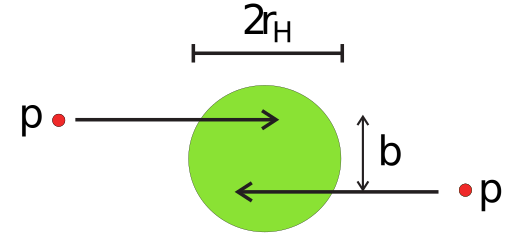
\includegraphics[width=6cm]{figures/bumm.pdf}}
\hspace{1cm}
\subcaptionbox{Quantum Black Hole\label{fig:add-boundary}}%
   [.4\linewidth]{\includegraphics[width=6cm]{figures/hossi-minibh.pdf}}
}% makebox
\caption[Illustrations for large extra dimensional concepts, modified from \cite{KBH2005,cavaglia,Hossenfelder2004}]{Illustrations on how to imagine large extra dimensions and brane world physics.

(a) The (orange) 4d branes are displayed as 2d surfaces, while one extra dimension is displayed horizontally. While the QED process takes place on the brane, and neither electron, positron and photon can escape the brane, the graviton is allowed to freely traverse the whole space-time.

(b) The compactification picture shows where one faces extra dimensions even in real life: When zooming in, the one dimensional horizontal line shows a vertical substructure. At big distances, the extra dimensions are not visible.

(c) The hoop conjecture illustration shows how to imagine a particle collision with impact parameter $b<2 r_H=2 L_*$ which produces a black hole with event horizon $2R_H$.

(d) A black hole with $r_H \ll R_c$, that is, the BH is much smaller than the compactification radius of the tori, does not notice the extra dimensional periodic boundary geometry.

Pictures taken and adapted from \cite{KBH2005,cavaglia,Hossenfelder2004}.}\label{fig:lxd-1}
\end{figure}

\begin{figure}
\centering
\includegraphics[scale=1]{figures/ADD-fundamental-mass.pdf}
\caption[ADD fundamental mass lowering principle plot/illustration]{The ADD fundamental mass lowering mechanism. The lines show $M_*(R_c)$ from eq. \eqref{eq:mstar-convention} on a GeV scale. For comparison, the LHC energy scale (10 TeV) is shown, as well as the Planck scale ($n=0$). Instead of including real world values for $R_c$ or $C_n$, the plot illustrates the mechanism: By gravitational experiments, one can make upper bound constraints on $R_C$. Small number of extra dimensions, like $n=1$, are ruled out because they reach the TeV scale only at very large distances.}\label{fig:ADD-fundamental-mass}
\end{figure}

\subsection{The Schwarzschild-Tangherlini solution}
Black holes in higher dimensions are more diverse than in 4d, since more topologies are possible \cite{ReallLRR}, for example ring solutions (``black rings'', like Doughnuts). The most simple generalization of the Schwarzschild solution to $d$ dimensions is the \emph{Schwarzschild-Tangherlini} metric (STM). It describes the spherical and static black hole produced by a point like matter source in higher dimensions and was found in 1963 by Tangherlini. The metric is displaye by the line element
\begin{equation}\label{eq:metric-schwarzschild-n}
\d s^2 = - (1-V(r)) \d t^2 + (1-V(r))^{-1} \d r^2 + r^{d-2} \d \Omega_{d-2}^2.
\end{equation}
This line element is a straightforward extension of the 4d Schwarzschild line element \eqref{eq:metric-schwarzschild-1}. The gravitational function is retrieved by replacing the $1/r$ Newtonian  radial falloff by $1/r^{d-3}$, getting \cite{ReallLRR}
\begin{equation}\label{eq:schwarzschild-grav-potential}
V(r) = \frac{2}{d-1} \frac{M G_d}{r^{d-3}} = \left( \frac{r_H}{r} \right)^{d-3},
r_H^{d-3} = \frac{d-1}{2} M G_*
\,,
\end{equation}
with the $d$-dimensional coupling constant $G_d$ and mass parameter $M$. The modification of the coupling constant is a crucial reason why extradimensional gravity is done and subject to the following section. The $d$-dimensional coupling constant $G_d$ will be refered to as $G_*$. The number of dimensions arises from the context. Writing the gravitational potential in terms of the horizon radius \eqref{eq:schwarzschild-grav-potential} uncovers the \emph{no more} linear size-mass relation $r_H \propto M$, It is only linear in 4 dimensions.

%The Schwarzschild-Tangherlini metric \eqref{eq:metric-schwarzschild-n} will be derived as the point like mass distribution limit in section \ref{sec:generic-H}.

\clearpage
\section{Black Holes in Large Extra Dimensions}
\subsection{Production}
There is no accelerator on Earth which can probe quantum gravity at the Planck scale $\sim 10^{16}$ TeV, as already mentioned in section \ref{sec:planck-scale}. On the contrary, the ADD scenario allows black holes production in particle accelerators.

By means of the \emph{hoop conjecture} (figure \ref{fig:hoop-conjecture}), black holes are produced as soon as $M_\text{center of mass} \sim M_*$. As $L_* \ll R_c$, no problems arise with the special enrolled nature of the spatial extra dimensions (figure \ref{fig:add-boundary}): The black hole is very small compared to the extra dimensional tori, so it locally looks $3+n$-spherically symmetric \cite{Hossenfelder2004}.

The production rate is governed by a geometrical cross section approximation
\begin{equation}
\sigma(M) \sim \pi r_H^2.
\end{equation}
This experimental signature is the main motivation for investigating black holes in large extra dimensions \cite{Gingrich:2010ed,Giddings2014,ScardigliCasadio2014}.

%In the first three year LHC run, no black holes where detected.
%
%For literature about the experimental setup and observation of black holes in particle accelerators like the LHC, see e.g. \cite{cavaglia,Kanti2004,Kanti2014,BN2010,KBH2005,Bleicher2013,miniReview}.


\subsection{Evaporation}\label{sec:evaporation}
Mini black holes produced in particle colliders evaporate by Hawking radiation, because their lifetime is very short, compared to their astronomical counterparts. The evaporation process is typically categorized in four phases \cite{miniReview,KBH2005,Hossenfelder2004}:

%
\begin{enumerate}
%
\begin{minipage}{0.55\linewidth}
\item[(a)] {\bf Balding phase}. In this phase the black hole looses \emph{hair} which consist of asymetries (multi-pole moments and gauge fields, if applicable). It is expected that the BH goes throught the balding phase very rapidly \cite{Winstanley2007}. At the end of this phase, the BH is axisymmetric and rotating. This kind of BH is described by the Kerr-Newman metric.

\item[(b)] {\bf Spin down phase}. The black hole radiates away all of its angular momentum and some mass. The evaporation is understood in terms of Hawking and Unruh-Starobinsky radiation. At the end of this phase, the BH is spherical symmetric and nonrotating. This kind of BH is described by the Schwarzschild metric.

\end{minipage}
%\hspace{.5cm}
\hfill{}
\begin{minipage}{0.4\linewidth}
%\begin{figure}
%\begin{wrapfigure}[12]{r}[1cm]{5cm}
\includegraphics[width=\textwidth]{figures/bhphase-ab.pdf}
\captionof{figure}[Illustrations of the evaporation phases, taken and modified from \cite{Hossenfelder2004}]{Sketch of the phases, modified from \cite{Hossenfelder2004}}\label{fig:evaphases1}
%\end{wrapfigure}
%\end{figure}
\end{minipage}
\end{enumerate}

\begin{figure}[h!]
\includegraphics[width=0.8\textwidth]{figures/bhphase-cd.pdf}
\caption[Illustration about the evaporation phases, taken and modified from \cite{Hossenfelder2004}]{Sketch of the evaporation phases, modified from \cite{Hossenfelder2004}.}\label{fig:evaphases2}
\end{figure}

\begin{enumerate}
\item[(c)] {\bf Schwarzschild phase}. The black hole is spherical and still radiates by Hawking radiation (monopole radiation).

At the end of this phase, the semiclassical thermodynamics, based on the Hawking temperature
\begin{equation}
T_H = \frac{\hbar}{8\pi GM},
\end{equation}
get more and more \emph{ill defined}. The evaporating black hole gets hotter and hotter and evventually emits particles with the same order of mass as the black hole mass. The thermodynamical canonical ensemble gets wrong because the black hole cannot be in a stable equilibrium with its surrounding heat bath any more \cite{frolov}.

\item[(d)] {\bf Planck phase}. The black hole mass reaches the Planck mass and quantum gravity effects get strong. In this phase, $r_H \sim L_*$ and the semiclassical picture breaks down. There are two widely acknowledged opportunities: The black hole completely evaporates away to particles of the Standard Model, or it gets a stable configuration, the \emph{black hole remnant}.
\end{enumerate}

%Figure \ref{fig:evaphases} illustrates these phases.


\chapter{Minimal length in physics}\label{sec:minial-length}
This chapter is devoted to the minimal length issue in general relativity and quantum mechanics. There are two short scale problems addressed on the next pages: The curvature singularity at the origin of the Schwarzschild black hole which may be backtraced to the Dirac delta distribution composing the matter source $\delta(\bv x)$. The Dirac distribution is a good model (in the sense of a matter profile) as seen from a far from the origin, while it fails at small distances from the origin. As one of the tenets of physics is the association of the failure of a theory at scales where the theory predicts divergences, the Schwarzschild metric must be replaced at short scales.

The second problem proposed on the next pages is a duality problem at scales where quantum mechanics get important. Most quantum gravity approaches address these two short scale problems by \emph{nonlocality}. The nonlocality is typically intermediated by a minimal length scale which corresponds to an energy scale when nonlocal effects become strong \cite{AuriliaSpallucci2013b,Casadio:2014pia,HossenfelderLRR,AdlerSixRoutes}. It is the aim of this chapter to show that it is sufficient to include nonlocal effects in general relativity instead of replacing it with another theory. The generalized uncertainty principle (GUP) is given as an example theory supporting this line of reasoning. Other approaches producing short-scale improved black holes are given in appendix \ref{sec:apx-qgbhs}.


\section{The black hole---particle duality}\label{sec:bh-particle-duality}
At Planck length and Planck mass scales there is a tangible particle-black hole \emph{duality}, illustrated in figure \ref{fig:bh-duality-SSM}. This duality is derived as follows: On the quantum mechanical side, it is possible to assign each particle with mass ($=$energy) $m$ a length $\lambda$, which is typically interpreted as a wave length in the wave--particle duality. It is the \emph{de Broglie wavelength} $\lambda_B = h/p$ or in the limit $v\to c$ the \emph{Compton wavelength} $\lambda_C = \hbar / mc$. To approach the Planck length, consider the Compton wavelength $L_\text{particle} \sim 1/m$. It is displayed by the red curve in figure \ref{fig:bh-duality-SSM}. Note that \emph{Feynman units} with $2\pi \approx 1$ are used, \emph{i.e.} numerical factors are suppressed in this picture \cite{AdlerSixRoutes}.

On the other hand, the black hole picture in four space-time dimensions assigns to each mass distribution a length by means of the Schwarzschild event horizon $r_H = 2GM/c^2$, so $L_\text{black hole} \sim m$, as the blue curve indicates. These two curves cross at the Planck scale $L_\text{particle} \sim L_\text{black hole} \sim \sqrt{\hbar c/G} := L_\text{Pl}$.

Trace as a gedankenexperiment a particle in an accelerator where its energy (velocity) is increased, resulting in a better length scale resolution (particle compression, red arrow). At the Planck scale $M_\text{pl}$, suddenly by the \emph{hoop conjecture} (figure \ref{fig:hoop-conjecture}) one expects the particle to become a black hole, and further energy (i.e. acceleration) increases the size of the object (again). The resulting black hole is quite unstable and decays by Hawking evaporation (blue arrow). As one does not expect a reversing mechanism of the hoop conjecture (which may be called \emph{inverse hoop conjecture}), nothing prevents the Schwarzschild black hole from evaporating at scales below the Planck scale. One ends up with a situation where two theories predict two different sizes for the same energy scale: A particle in quantum mechanics and a black hole in general relativity.

Note that in the extra dimensional scenario, the black hole mass--length ratio is no longer proportional, but $L_\text{black hole} \sim \sqrt[2+n]{m}$. The situation is displayed for different choices of $n$ in figure \ref{fig:bh-duality-STM}. The modified mass--length relation does not change the qualitative nature of the black hole--particle duality, for each number of extra dimensions the above statement holds.

\begin{figure}
\centering
\begin{subfigure}{0.5\textwidth}
\caption{BH--particle duality in 4 dimensions}\label{fig:bh-duality-SSM}
\includegraphics[width=\textwidth]{figures/completeness-schwarzschild.pdf}
\end{subfigure}%
\begin{subfigure}{0.5\textwidth}
\caption{BH--particle duality in $n$ LXDs}\label{fig:bh-duality-STM}
\includegraphics[width=\textwidth]{figures/completeness-STM.pdf}
\end{subfigure}
\caption[Illustration about the black hole and particle phases]{Length-vs-mass pictures for the Schwarzschild(-Tangherlini) space time (blue lines) vs the quantum mechanical picture (red dashed line)}\label{fig:bh-duality-SS}
\end{figure}

\section{Self-Completeness}
There are two ways out of the black hole--particle ambiguity: Either general relativity breaks down and must be replaced by a completely different theory, or it can be saved by some kind of \emph{completeness}. The completeness paradigm is sketched in figure \ref{fig:bh-fake-gup} and defined as follows: By modifying the gravitational event horizon in a way that it smoothly merges into the particle picture, one gets a unique particle--black hole interpretation and a \emph{minimum length scale} of physics $l_0$. In a theory implementing this completeness paradigm, there is literally no way to probe distances below $l_0$ as it is either circumvented by quantum mechanical uncertainity or black hole production. The theory is called \emph{self}-complete, if $l_0$ is the fundamental mass scale of the theory. For example, a (modified) 4d Einstein-Hilbert action could be self-complete if $l_0=L_\text{Pl}$.

Gravity is called self-complete if the validity of the Einstein field equations (EFE) is recognized at any energy scale (i.e. mass scale $M$ at figure \ref{fig:bh-duality-SS}), but it is \emph{self protecting} against short length singularities \cite{dvali1}. This is imposed by completing the EFE by a nonlocal contribution. This modification is motivated by fundamental principles like the generalized uncertainty principle, noncommuting geometry or theories like loop quantum gravity and string theory \cite{Spallucci:2012xi,SpallucciReview}. Appendix \ref{sec:apx-qgbhs} gives a short overview about these theories.


\begin{figure}[h!]
\floatbox[\capbeside\thisfloatsetup{floatwidth=\textwidth,capbesidewidth=sidefil,capbesideposition={right,top}}]{figure}[\FBwidth]{%
\caption[Illustrative sketch how self-complete gravity performs in the Mass--Length picture]{Self-complete gravity: The red line displays the unaltered length scale associated with quantum particles, while the green line is an exemplary placeholder for a quantum gravity improved black hole horizon. The picture suggests a ``smooth'' transition at the Planck scale $M=M_\text{PL}, L=L_\text{Pl}$. In this way, the length scales $L<L_\text{Pl}$ are no more physically accessible.

This picture shall be understood as the goal of the short scale improved black hole metrics which are subject of the following chapters.
}\label{fig:bh-fake-gup}
}{\includegraphics[width=8cm]{figures/completeness-gup-fake-holo.pdf}}
\end{figure}

\section{Nonlocal gravity}\label{sec:nonlocal-gravity}
The nonlocal contributions to the geometric part of the Einstein field equations are introduced with a bilocal operator $\C A^2$ which mediates \emph{nonlocal} effects in space-time. $\C A^2$ is a function of the generally covariant D'Alambert operator $\square = g^{\alpha\beta} \nabla_\alpha \nabla_\beta$ associated with an energy scale $1/l_0$ which is generated by the physical length scale $l_0$ at which short distance effects get important. $\C A^2(\square~l_0^2)$ is a dimensionless and generally covariant operator. To shorten notation, it will frequently be abbreviated as $\C A^2$. It enters the Einstein field equations on the right hand side of Einstein equations as the inverse $\C A^{-2}$,
\begin{equation}\label{eq:Mod-Einstein1}
G_{\mu\nu} = -8\pi G~ \C A^{-2} T_{\mu\nu}
:= -8\pi G \C T_{\mu\nu}.
\end{equation}
The non-classical matter distribution $\C T_{\mu\nu} = \C A^{-2} T_{\mu\nu}$ is described by the nonlocal operator. By multiplying the inverse $\C A^{2}$ of $\C A^{-2}$ from the left hand side, the \emph{dual theory} is found:
\begin{equation}\label{eq:Mod-Einstein2}
\C A^2 ~G_{\mu\nu} := \C G_{\mu\nu} = -8\pi G~ T_{\mu\nu}.
\end{equation}
In the dual theory, the nonlocality is \emph{shifted} to the geometrical part (the Einstein tensor) of the field equations, while the matter part remains purely classical.

Note the difference between equation \eqref{eq:Mod-Einstein1} and \eqref{eq:Mod-Einstein2}: While the field equations \eqref{eq:Mod-Einstein1} represents classical gravity coupled to a non-local source term $\C T_{\mu\nu}$, the field equations \eqref{eq:Mod-Einstein2} describe equations for a nonlocal Einstein tensor $\C G_{\mu\nu}$ representing a modified geometry coupled to a classical source term $T_{\mu\nu}$. These two interpretations are (mathematically and physically) equivalent \cite{NFeb2012,MMN2010}.

The action of the nonlocal field theory is obtained by inserting the modified Ricci scalar $\C R$ in the Einstein-Hilbert action \eqref{eq:Einstein-Hilbert-action}.

%
%\subsection{Acting on the Dirac delta distribution}
%The nonlocal effect of $\C A^2$ can be separated by displaying the Ricci scalar with a Dirac delta distribution
%\begin{equation}
%\C R(x) = \C A^2(\square_x~l_0^2) R(x)
%= \int \d y~ \CA^2(\square_x~l_0^2) \delta(x-y) R(y).
%\end{equation}
%By means of the momentum representation of the dirac distribution $\delta(x)=\int \d p~e^{ipx}$, the nonlocal operator $\C A^2$ can be displayed in momentum space:
%\begin{equation}
%\C R(x) = \int \d y~R(y) \int \d p
%\C A^2(-p^2) e^{ip(x-y)}.
%\end{equation}

\section{The generalized uncertainty principle}
The generalized uncertainty principle (GUP) is one way to find a minimal length scale in physics \cite{Adler2001,Casadio:2013tza}. It proposes a modification of the Heisenberg uncertainty principle
\begin{equation}
\Delta x \, \Delta p \geq \frac{\hbar}{2}.
\end{equation}
As the Heisenberg uncertainty principle is a consequence of the quantum mechanical commutator relation $[\bv x, \bv p] = i\hbar$, the GUP is usually introduced by complementing this commutator relation for momentum and/or position dependent terms \cite{Kempf1994},
%
\begin{equation}
[\bv x, \bv p] = i\hbar (1 + \alpha \bv x^2 + \beta \bv p^2).
\end{equation}
This yields a modified uncertainty relation of the form
\begin{equation}\label{eq:GUP-relation-generic}
\Delta x \, \Delta p \geq \frac{\hbar}{2}
\left( 1 + \alpha \bv x^2 + \beta \bv p^2 + \alpha \langle \bv x\rangle^2 + \beta \langle \bv p \rangle^2 \right).
\end{equation}

\begin{wrapfigure}{r}{6cm}
\vspace*{-1cm}
\begin{center}
\includegraphics[scale=1]{figures/completeness-simple-gup.pdf}
\end{center}
\vspace*{-0.5cm}% Caption nach oben rutschen  
\caption[The Length-vs-Mass picture for the GUP]{The GUP predicts a minimal length (green dot). Here, $\beta=2$ and $\hbar=1$.
}\label{fig:bh-real-gup}
\label{fig:completeness-halpha}
\end{wrapfigure}

Restricting to the case $\alpha=0$ allows to find a Hilbert Space representation \cite{Kempf1994} in momentum space. Solving relation \eqref{eq:GUP-relation-generic} for exact equality for $\Delta p$ requires for exact momentum measurement $\langle p \rangle = 0$ a minimal position uncertainty
\begin{equation}
\Delta x \geq \hbar \sqrt{\beta}.
\end{equation}
It is possible to derive a black hole solution based on this priniciple which implements a \emph{smearing} of point-like mass distributions \cite{Isi1,Isi2,Knipfer2014,Marco,GUPpaedagogical}. The GUP can also be expressed as a nonlocal field theory. For further details, see appendix~\ref{sec:apx-gup}, as a complete discussion is beyond the scope of this work. 

%
%\begin{figure}[h!]
%\floatbox[\capbeside\thisfloatsetup{floatwidth=\textwidth,capbesidewidth=sidefil,capbesideposition={right,top}}]{figure}[\FBwidth]{%
%\caption[TODO {\bf PENDING} GUP plot]{The outer horizon of the spherical static black hole in the GUP scenario (blue), compared to the classical Schwarzschild prediction (black). The green range indicates the accessible range predicted by the uncertainty relation \eqref{eq:GUP-relation-generic}. The lower bounds of the compton wavelength and GUP black hole horizon allow a greater accessible physical region. In any way, distances below $L < L_*$ cannot be probed.
%}\label{fig:bh-real-gup}
%}{\includegraphics[width=8cm]{figures/completeness-real-gup.pdf}}
%\end{figure}


\chapter{Quasi-classical black holes}\label{sec:generic-H}
In this chapter, a class of generic black hole solutions is introduced. This is done as a preparatory effort to derive the mathematical equations used to discuss two physically motivated subclasses of black holes in the next two chapters.

The class of black holes described in this chapter is constructed by a quasi-classical source term which models a \emph{smeared} Dirac delta distribution. This is one way to introduce nonlocal gravity effects. Such effects turn out to be successful to encounter the problems of the Schwarzschild black hole, discussed in the previous chapters. The modifications from the ordinary Schwarzschild setup are supposed to be large only at short distances around the center, while at large distance, all metrics in the currently discussed class of generic \emph{smeared} Schwarzschild black holes shall match the ordinary Schwarzschild black hole.

In the static radial symmetric setup, we can compute the modifications from the ordinary Schwarzschild setup. In this chapter, a concrete choice for the smearing will not be made. It is introduced only in a fashion $\Theta(r) \to H(r)$ with $\Theta(r)$ the Heaviside step function and $H(r)$ an approximation function, characterized by a regulator $\tilde r_0$ with dimension of length. As we will derive a nonlocal operator for this class of black holes in the end of the chapter, $\nicefrac 1{\tilde r_0}$ turns out to be the energy scale where modifications to general relativity apply. These modifications are encoded in $H(r)$. According to $H(r)$, the modifications can improve the low distance regime of general relativity.


\begin{figure}
\centering
\begin{subfigure}{0.45\textwidth}
\caption{Heaviside step function $\Theta(r)$}\label{fig:diracH-heaviside}
\includegraphics[width=\textwidth]{figures/diracH-heaviside.pdf}
\end{subfigure}%
\hspace{0.02\textwidth}
\begin{subfigure}{0.45\textwidth}
\caption{Dirac delta function $\delta(r)$}\label{fig:diracH-dirac}
\includegraphics[width=\textwidth]{figures/diracH-dirac.pdf}
\end{subfigure}%

\begin{subfigure}{0.45\textwidth}
\caption{Heaviside-approximation $H(r)$}\label{fig:diracH-holo}
\includegraphics[width=\textwidth]{figures/diracH-holo.pdf}
\end{subfigure}%
\hspace{0.02\textwidth}
\begin{subfigure}{0.45\textwidth}
\caption{Dirac-approximation $H'(r)$}\label{fig:diracH-dholo}
\includegraphics[width=\textwidth]{figures/diracH-dholo.pdf}
\end{subfigure}
%
\caption[Illustrative plots, comparing point-source describing functions with their smeared, delocalized ones.]{Illustrative plots to emphasize the impact of replacing $\delta(r) \to H'(r)$ or $\Theta(r) \to H(r)$, respectively, in the Schwarzschild matter distribution. The exact definition of the Heaviside step function \ref{fig:diracH-heaviside} at the origin $r=0$ is not important here. Note that the smearing is not performed around the origin $r=0$, but in a manner that $H(0)=0$ is ensured. Else, the physical interpretation of $H(r)$ as a matter distribution would be lost, as $r<0$ is not a valid position in spherical coordinates. The \emph{amount} of delocalization is supplied by the length scale $\tilde r_0$. For illustration purpose, here $H(\tilde r_0)=H'(\tilde r_0)= \nicefrac 12$. Note that for $\tilde r_0 \to 0$, the approximation functions $H(r)$ and $H'(r)$ match their ideal $\Theta(r)$ or $\delta(r)$, respectively.}%
\label{fig:delta-smearing}
%
\end{figure}

\clearpage
\section{From a quasi-classical source term to the metric}\label{sec:derivation-metric-H}
In this section, the metric for any static spherical symmetric gravitational potential $V(r)$ in $d$ space time dimensions will be derived. As the ADD model is used, the $d$ dimensions are spanned by $1$ timelike and $d-1=n+3$ spacelike dimensions, where $n$ indicates the number of extradimensions.

The only further requirement is large distance matching of the Netwon's potential \eqref{eq:newton-potential}. This is equivalent to starting with a static isotropic matter density $\rho(r)$ and requiring $\lim \limits_{r\to\infty} \rho(r)=0$.

The ansatz for the solution is the following $d=n+4$ dimensional spherical symmetric and static metric, described by a line element
\begin{align}\label{eq:Schwarzschild-ndim-V}
\d s^2 &=
- e^{\nu(r)} \d t^2
+ e^{-\nu(r)} \d r^2
+ r^2 \d \Omega_{n+2}^2
\\ &=
- \left( 1 - V(r) \right) \d t^2
+ \left( 1 - V(r) \right)^{-1} \d r^2
+ r^2 \d \Omega_{n+2}^2
\end{align}
with $\Omega_{n+2}$ the surface line element of an $(n+3)$ sphere (for details about the sphere, see appendix~\ref{section:apx-spheres}). The spherical coordinates are given by $\bv x = (x_0, \vec x) = (x_0, r, \phi, \theta_1, \dots, \theta_{n+2})$. To improve readability, it is written $i$ instead of $\theta_i$ ($i=1,\dots,m$ and $m:=n+2$) when the angular coordinates appear in the indices of tensors. The diagonal coefficients in the metric are therefore refered to as
\begin{equation}
g_{AB} = \diag \left(
g_{00}(r), -g_{00}^{-1}(r),
g_{\phi\phi}(r,\phi),
g_{11}(r,\theta_1),
\dots,
g_{mm}(r,\theta_m)
\right).
\end{equation}
This notation is the same as in \cite{Rizzo}.

The argumentation follows the derivation of the inner Schwarzschild solution, as can be found in general relativity textbooks: The property $-g_{00} = g_{11}^{-1}$ is required for flat space at large distances.

Given the matter density and the metric ansatz, the stress tensor $T^{AB}$ can be determined. Due to the symmetry of the problem, it can already be stated as
\begin{equation}\label{eq:T-Ansatz}
T^{AB}
= \diag\left(
T^{00}, T^{rr},
T^{\phi\phi},
T^{11},
T^{22},
\dots,
T^{mm},
\right)
= \diag\left(
-\rho, -\rho, p, p, \dots, p
\right),
\end{equation}
following \cite{Rizzo, NSS2006}. Now switching to a $(1,1)$ type tensor for $\bv T$ yields the conservation of energy equation as $\nabla_A T^A_B=0$ with
\begin{equation}
T^A_B = g_{BC} T^{AC}
= g_{BB} T^{AB}
= \diag(g_{00} T^{00}, g_{rr} T^{rr}, \dots, g_{mm} T^{mm}).
\end{equation}
The conservation equation $\nabla_A T^A_B=0$ is now computed for all $d$ possible values of the free index $B$. Starting with the index $B=r$ case gives the equation (no sum convention here)
\begin{equation}\label{eq:Trr-derivation}
0 = \nabla_0 T^0_r + \nabla_r T^r_r
+ \sum_i \nabla_i T^i_r.
\end{equation}
The covariant derivative $\nabla_A$ and the Christoffel symbol $\Gamma_{AB}^C$  must be computed (see appendix~\ref{sec:formelsammlung} for the definitions). The summands of \eqref{eq:Trr-derivation} are given by
\begin{subequations}
\begin{align}
\nabla_0 T^0_r &=
\partial_0 T^0_r
+ \Gamma^0_{0D} T^D_r
- \Gamma^D_{0r} T^0_D
=
\frac 12 g^{00} T^r_r \partial_r g_{tt} +
\frac 12 g^{00} T^0_0 \partial_r g_{tt}
\\
\nabla_r T^r_r &=
\partial_r T^r_r
+ \Gamma^r_{r D} T^D_r
- \Gamma^D_{r r} T^r_D
= \partial_r T^r_r
\\
\forall i:\quad
\nabla_i T^i_r &=
\partial_i T^i_r
+ \Gamma^i_{i D} T^D_r
- \Gamma^D_{0 r} T^i_D
=
\frac 12 g^{ii} T^r_r \partial_r g_{ii} +
\frac 12 g^{ii} T^0_0 \partial_r g_{ii}
\end{align}
\end{subequations}
One ends up with the explicit equation %already seen in \cite{Rizzo}
\begin{equation}
0 = \partial_r T^r_r
+ \frac 12
g^{00} \left( T^r_r - T^0_0 \right) \partial_r g_{00}
+
\frac 12
\sum_i
g^{ii} \left( T^r_r - T^i_i \right) \partial_r g_{ii}
\end{equation}
By construction of $T^A_B$, the term $T^r_r - T^0_0\sim \rho-\rho=0$ vanishes. The remaining contribution from each angle $i$ is
\begin{equation}\label{eq:remaining-sinii}
g^{ii}\partial_r g_{ii}
=
\frac 1{ r^2 \sin^i(\theta_i) }
\partial_r
\left(
r^2 \sin^i(\theta_i)
\right)
= \frac 2r,
\end{equation}
where $\sin^i(x)=\left(\sin(x)\right)^i$ displays the $i$th power of $\sin(x)$. By summing up $d-2$ equal terms \eqref{eq:remaining-sinii}, all remaining energy momentum components are determined to
\begin{equation}\label{eq:outward-pressure}
T^i_i = T^0_0 + \frac r{n+2} \partial_r T^0_0
=  \rho + \frac r{n+2} \partial_r \rho.
\end{equation}
As a result, the index $B=r$ case of the energy conservation law $\nabla_A T^A_B=0$ already determined the energy momentum tensor. It is not shown here that the other $d-1$ energy conservation equations do not contribute any further information.

In order to solve the Einstein equation, in addition to the energy momentum tensor one needs the Ricci tensor as additional ingredient. It is given as the contraction of the Riemann tensor
\begin{equation}
% griechische indices:
%R_{\mu\nu} = 
%\partial_\lambda \Gamma^\lambda_{\nu\mu} -
%\partial_\nu \Gamma^\lambda_{\lambda\mu} +
%\Gamma^\lambda_{\mu \gamma} \Gamma^\gamma_{\nu\mu} -
%\Gamma^\lambda_{\nu\gamma} \Gamma^\gamma_{\lambda \mu},
%
% gross lateinische:
R_{AB} =
  \partial_C \Gamma^C_{BA}
- \partial_B \Gamma^C_{CA}
+ \Gamma^C_{AD} \Gamma^D_{BA}
- \Gamma^C_{BD} \Gamma^D_{CA}
\end{equation}
see Appendix \ref{sec:apx-christoffels} for the values of all Christoffel symbols. The Ricci tensor is again diagonal, with the entries, as (1,1) type tensor,
\begin{subequations} \label{eq:derivation-ricci-tensor}
\begin{align}
R^0_0 = R^r_r &= - \frac{e^\nu}2
\left( \partial_r^2 \nu + (\partial_r \nu)^2
+ (n+2) \frac{\partial_r \nu}r
\right)
=
\frac 12 V''(r) - \frac{n+2}{2} \frac{V'(r)}{r}
\\
\forall i:\quad R^i_i &=
\frac{1 + n - e^\nu
\left( 1 + n + r \partial_r \nu \right)
}{r^2}
=
(1+n)\frac{V(r)}{r^2} + \frac{V'(r)}{r}.
\end{align}
\end{subequations}
%
The Ricci scalar is then given by
\begin{equation}
R = R^A_A = \frac{(n+2) V(r)}{r^2}+V''(r).
\end{equation}

Now one can write out the Einstein equations in a trace reversed form, in $(1,1)$ tensor notation for $d$ dimensions:
\begin{equation}
R^B_A = \frac{1}{M_*^{n+2}}
\left(
T^B_A - \delta^B_A
\frac{T^C_C}{n+2}
\right)
\end{equation}
Since ${\bv R}, {\bv T}, {\bv \delta}$ are diagonal, the Einstein equations reduce to $d$ non-zero equations where only two equations differ from each other, identified by their indices $A,B=r,r$ and $A,B=i,i$. The latter gives the following first order differential equation for $V(r)$:
\begin{equation}
V'(r) + \frac{n+1}{r} V(r)
= \frac{1}{M_*^{n+2}} \frac{r \rho(r)}{n+2}
\end{equation}
The general solution of the metric for any $\rho(r)$ is given by the integral
\begin{equation}\label{eq:Rizzo-sol}
V(r) = \frac{1}{r^{n+1}}
\left(
\frac{1}{(n+2)M_*^{n+2}}
\int \limits_{c_1}^r
x^{n+2} \rho(x) \d x
+ c_2
\right)
\quad
\text{with} \quad c_1, c_2 = \operatorname{const}
\end{equation}
The boundary values $V(0)$ and $V'(0)$ give rise to the two integration contants $c_1$ and $c_2$. Physically, they allow for the low-energy matching of the theory. In the context of this thesis, $c_1$ is important for discussion about minimal lengths.

\section{A smeared point-like matter density}
The matter density choice to be inserted into \eqref{eq:Rizzo-sol} is based on the Schwarzschild-Tangherlini point-like static and spherically symmetric density
\begin{equation} \label{eq:rho-SSM-ndim}
\rho(r) = \frac{M}{\Omega_{n+2} ~r^{n+2}} \delta(r) = \frac{M}{\Omega_{n+2} ~r^{n+2}}
\dd{\Theta(r)}{r},
\end{equation}
with the Dirac delta distribution $\delta(r)$ and the Heaviside unit step function
\begin{equation} \label{eq:def-theta}
\Theta(r) = \begin{cases}
0 \quad \text{when}~~ &r < 0 \\
1 & r \geq 0
\end{cases}.
\end{equation}
The occurence of the Heaviside function in the Schwarzschild source term \eqref{eq:rho-SSM-ndim} is now replaced by a \emph{smeared} version we refer to as $H(r)$. By construction, the function $H(r)$ encodes all nonlocal effects of the theory. The generic \emph{Schwarzschild-like} energy density is therefore
\begin{equation} \label{eq:rho-H-ndim}
\rho(r) = \frac{M}{\Omega_{n+2} ~r^{n+2}} \dd{H(r)}r.
\end{equation}
Inserting \eqref{eq:rho-H-ndim} into the integral \ref{eq:Rizzo-sol} gives us the \emph{gravitational function} $V(r)$ with $n$ large extra dimensions as
\begin{equation}\label{eq:V-for-generic-H}
\highlight{
V(r) = \frac{1}{2+n} \frac{M}{M_*^{n+2}} \frac{H(r)}{r^{n+1}}.
} %eoh
\,.
\end{equation}
%
Here, $M_*$ is the fundamental Planck mass, and $M$ is a constant that will be identified as mass. $V(r)$ determines the metric according to
\begin{revisited}{eq:Schwarzschild-ndim-V}
\d s^2 =
- \left( 1 - V(r) \right) \d t^2
+ \left( 1 - V(r) \right)^{-1} \d r^2
+ r^2 \d \Omega_{n+2}^2.
\end{revisited}
The gravitational function $V(r)$ replaces the Newton's potential \eqref{eq:newton-potential} with a prefactor $-2$, because plugging $V(r)=-2\Phi(r)$ with $\Phi(r)=-GM/r$ into \eqref{eq:Schwarzschild-ndim-V} resembles the Schwarzschild solution.

\subsection{The Mass}\label{sec:mass}
%\todo[inline,color=blue!40]{{\bf Question}: Shall I mention the bad definition of the mass, sinc the line element in integral \eqref{eq:M-integral} is actually {\bf wrong} and should be $\sqrt{-g}\d^{n+3} x$? Current papers (e.g. Ansoldis Review about regular BHs) do not discuss this, but some textbooks about GR do. Do you have literature where this is discussed for our class of QG black holes?}
The mass contained inside a $(3+n)$-sphere (the object will be referred to as $\C B(r)$) with radius $r$ is given by the integral
\begin{equation}\label{eq:M-integral}
m(r) = \int \limits_{\C B(r)} \rho(x) ~\d^{n+3} x
= M \int \limits_0^r \dd Hr (r') ~\d r' = M H(r).
\end{equation}
%
%From the physical viewpoint, this is the mass visible to any observer outside this sphere, that is, at position $r' > r$. Note that actually, we make a small mistake, because the correct integral measure would be
%\begin{equation}
%\int_{\C B(r)} \sqrt{-g}~\d^{n+3} x~\rho(x),
%\end{equation}
%but everybody does that.

From the mathematical viewpoint, the mass $M$ is just a constant that may be used to fulfill the horizon equation $V(r_H)=1$ at an arbitrary event horizon $r_H$. Therefore I set
\begin{equation} \label{eq:M-for-generic-H}
M := (n+2) M_*^{n+2} \frac{r_H^{n+1}}{H(r_H)},
\end{equation}
so when plugging into the metric
\begin{equation} \tag{\ref{eq:V-for-generic-H} revisited}
V(r) = \frac{1}{n+2}
\frac{M}{M_*^{n+2}}
\frac{H(r)}{r^{n+1}}
=
\left(\frac{r_H}{r}\right)^{n+1},
\end{equation}
the horizon equation $V(r)=1$ is fulfilled at $r=r_H$. The physical meaing of $M$ is the mass of a black hole of radius $r_H$ \cite{NS2013}. When substituting $n+1$ powers of $M_*$ by $M_* = 1/L_*$, one can easily relate %$M$ to $M_*$
\begin{equation}\label{eq:Mass-rH}
\highlight{
M = (n+2) \left( \frac{r_H}{L_*} \right)^{n+1}
\frac{1}{H(r_H)} M_*
}%eoh
\,.
\end{equation}

%Todo: ADM Mass

\subsection{The regulator}\label{sec:regulator}
The ``spread'' of \emph{smearing} accomplished by the function $H(r)$ must be encoded in a constant of dimension length. For example, consider the Gaussian delta approximation
\begin{equation}
\delta_\sigma(r) = \frac{1}{\sqrt{2\pi\sigma}} \exp \left( - \frac{r^2}{2\sigma} \right),
\quad \delta(r) = \lim_{\sigma \to 0} \delta_\sigma(r).
\end{equation}
as a canidate for $H'(r) := \delta_\sigma(r)$. The variance $\sigma$, also refered to as the \emph{width} of the Gaussian, is the regulator of the metric constructed when inserting the cumulative normal distribution function $H(r) := \propto \int_{-\infty}^r e^{-x^2 / 2\sigma} \d x$ into \eqref{eq:V-for-generic-H}.

In the physical models in the next chapters, the \emph{width} (from now on the symbol $\tilde r_0$ will be generally used) will be linked to a physical length scale by imposing principles like self-encoding.

To take the limit $H(r) \to \Theta(r)$, one has to examine the limit of the regulator $\tilde r_0 \to 0$. The limit $\tilde r_0 \to 0$ is accomplished by the replacement rules
\begin{equation}\label{eq:regulator-replace}
H(r)\to 1, H'(r) \to 0, H''(r) \to 0, \dots.
\end{equation}
Replacing occurences of $H(r)$ and derivatives according to \eqref{eq:regulator-replace} only holds when evaluating expressions containing $H(r)$ and derivatives for nonzero radius. This resembles the well-known finite values of $\Theta(r)=1$ for $r>0$ and $\delta(r)=0$ for $r>0$.

This of course also holds for products like $H(r)H'(r)\to 0$.

\section{Geometry}
The mass $M$ and gravitational potential $V(r)$ have been determined for arbitrary $H(r)$. For specific choices of $H(r)$, one is able to do a discussion about event horizons ($g_{00} = 1 - V(r) \musteq 0$) and evventually draw a conformal diagram. This is done for two models in sections \ref{sec:geometry-holo} and \ref{sec:geometry-halpha}. Here, the discussion will be a general one about special features of any metric described by $H(r)$.

\subsection{Remnants}
Nonlocal matter distributions described by $H(r)$ exhibit extremal configurations which can be identified with the two \emph{remnant equations}, also known as \emph{degenerate horizon conditions}:
%
\begin{numcases}{~}
\label{eq:remnant-eqs1}
  g_{00}(r_0) &= 0 \\
\label{eq:remnant-eqs2}
  \left. \partial_r \right|_{r=r_0} g_{00}(r) &= 0
\end{numcases}
%
The first equation \eqref{eq:remnant-eqs1} ensures the metric has a horizon at $r_0$. The second equation \eqref{eq:remnant-eqs2} requires the metric to have an extremal value at $r_0$.

As will be shown in section \ref{sec:T-for-H}, the second equation \eqref{eq:remnant-eqs2} also states that the extremal configuration temperature, which is propertional to $\partial_r g_{00}(r)$, shall vanish at $r_0$. It will be shown in section \ref{sec:general-thermo} that, if condition \eqref{eq:remnant-eqs2} is met, the extremal configuration is stable and decays no more. The situation motivates the name \emph{black hole remnant} for the black hole with horizon radius $r_H = r_0$.

When inserting the generic potential \eqref{eq:V-for-generic-H}, the remnant equations give
\begin{subequations}
\begin{align}
\label{eq:remnant-H-eq1}
g_{00}(r_0) = 0 &= 1 - \frac{1}{2+n} \frac{M}{M_*^{n+2}} \frac{H(r_0)}{r_0^{n+1}}
\\
\label{eq:remnant-H-eq2}
\left. \partial_r \right|_{r=r_0} g_{00}(r) = 0 &= H'(r_0) -(n+1) \frac{H(r_0)}{r_0}.
\end{align}
\end{subequations}

The shape of $H(r)$ determines if the second remnant equation \eqref{eq:remnant-H-eq2} is fulfilled, while the first remnant equation \eqref{eq:remnant-H-eq1} will always be fulfilled for $H(r)\neq\Theta(r)$. 
 % As $H(r)$ is supposed to approximate a step function, chances are good that \eqref{eq:remnant-H-eq2} is fulfilled for \emph{any} reasonable $H(r)$. Therefore, remnants are a property of nonlocal gravity. Physical meaningful remnants which are stable also have to fulfill \eqref{eq:remnant-H-eq1}.

\subsection{Curvature finitness}\label{sec:general-curvature}
According to \eqref{eq:derivation-ricci-tensor}, the Ricci scalar is given by
\begin{subequations}
\begin{align}
R(r) &= R^N_N = \frac{(n+2) V(r)}{r^2}+V''(r)
\\
\label{eq:R-for-H}
&= 
\frac{2}{2+n}
\frac{M}{M_*^{2+n}}
\frac{(2+n)^2 H(r) - 2(1+n) r H'(r) + r^2 H''(r)}{r^{3+n}}.
\end{align}
\end{subequations}

A profile $H(r)$ can produce a non-singular black hole origin if the nominator in \eqref{eq:R-for-H} has a taylor expansion at least of order $r^{3+n}$. When expanding $H(r)$ and its derivatives in a series expansion around $r=0$ as
\begin{align}
H(r) &= \sum_{n=0}^\infty \frac{H^{(n)}(0)}{n!} r^n
\approx H(0) + H'(0) r + \frac 12 H''(0) r^2,
\\
H'(r) &= \sum_{n=0}^\infty \frac{H^{(n+1)}(0)}{n!} r^n
\approx H'(0) + H''(0) r %+ \frac 12 H'''(0) r^2,
\\
H''(r) &= \sum_{n=0}^\infty \frac{H^{(n+2)}(0)}{n!} r^n
\approx H''(0) %+ H'''(0) r + \frac 12 H''''(0) r^2,
\end{align}
one can determine the leading term (biggest power of $r$) from the nominator in \eqref{eq:R-for-H} as
\begin{multline}
(2+n)^2 H(r) - 2(1+n) r H'(r) + r^2 H''(r)
\\
\sim (2+n)^2 H(0) + (3+2n+n^2) H'(0) r  + (\nicefrac 14 n^2 - n) H''(0) r^2
\\
\propto H(0).
\end{multline}
A regular black hole therefore fulfills the condition
\begin{equation}
H(r) = \C O( r^{3+n} )
\quad\text{at origin }~r=0.
\end{equation}

\subsection{Energy conditions}
Energy conditions in general relativity are a tool to put constraints on matter distributions (that is, energy-momentum tensors) in a way how some expects them to behave. They are formulated from a classical viewpoint and \emph{not} deduced from Einstein field equations or other first principles. Roughly speaking, they generalize the statement that one does not observe negative masses or regions of negative mass distribution \cite{Poisson}.

Approaches to quantum gravity regularly violate energy conditions, and by examining how and where they violate these conditions, one understands about the quantum nature in general relativity. For example, one expects energy conditions violate around the black hole center, e.g. violations occur in a region $r \lesssim l_0$ while they hold for $r \gtrsim l_0$, with $l_0$ a physical mass scale associated with the theory under discussion. As Ansoldi notes, this is cannot be taken for granted in a non linear theory as general relativity is \cite{Ansoldi2008}.

\clearpage % it was always breaked before...
The following energy conditions (EC) are checked:
%
\begin{itemize}
\item {\bf Null EC}, defined that for every (future) \emph{null} vectors $x^\mu$ the observed matter density
\begin{equation}
\rho_\text{obs} = T_{AB} x^A x^B
\end{equation}
is non negative, $\rho_\text{obs} \geq 0$. In words, this means a matter density $\rho_\text{obs}$ observed by a \emph{light ray} must be positive. A null vector fulfills $x_A x^A = - x_0^2 + x_1^2 + \sum_{i=2}^{3+n} x_i^2 = 0$, and if it is a \emph{future} null vector, $x_A>0~\forall$ possible indices $A$. Since $T_{AB} \sim \diag(-\rho, -\rho, p,\dots, p)$ one gets
\begin{equation}
\rho_\text{obs} \sim -\rho x_1^2 + \sum_{i=2}^{3+n} p x_i^2
= -\rho x_1^2 + p (x_0^2 - x_1^2) = -(\rho + p) x_1^2 + p x_0^2
\stackrel{!}{\geq} 0
\end{equation}
The negative contribution is governed by
\begin{subequations}
\begin{align}
f_\text{weak}(r) &:= \rho + p = 2\rho + \frac{r}{n+2} \partial_r \rho.
\\
\label{eq:EEC-Null-H}
&= \frac{2 M}{\Omega_{n+2}}
\left(
\frac{2 H'(r)}{r^{n+2}} + \frac{1}{n+2} \frac{H''(r)}{r^{n+1}}
\right)
\end{align}
\end{subequations}
In regions where $f_\text{weak}(r)>0$, it is violated. For $H\to\Theta$, \eqref{eq:EEC-Null-H} is exactly $0$ except at the origin. For any non-Dirac distribution, derivatives of $H$ are nonzero near the origin, and therefore the null energy condition is violated. Anyway, due to the form of $H(r)$ which is constrained according to figure \ref{fig:delta-smearing}, $f_\text{weak}(r)>0$ is only possible at regions around the origin.

\item {\bf Strong EC} requires the same as the null EC for any (future) \emph{timelike} vector $x^\mu$. We find it violated when $f_\text{strong}(r) > 0$, with
\begin{subequations}
\begin{align}
f_\text{strong}(r) &= \rho + (3+n) p \\
&= \frac{M}{\Omega_{n+2}}
\left( \frac{(4+n) H'(r)}{r^{n+2}} + \frac{3+n}{2+n} \frac{H''(r)}{r^{n+1}} \right).
\end{align}
\end{subequations}
The same as for the null EC holds: As $H'(r)$ and therefore also $H''(r)$ is equal to zero beyond some characteristic length scale $l_0$ according to the smearing principle displayed in figure \ref{fig:delta-smearing}, the strong EC is violated near the origin.

\item {\bf Dominant EC} requires for any (future pointing) timelike or null vector $x^\mu$ that $-T^A_B x^B=-T^A_A x^A=y_A$ is a future timelike or null vector. It requires both $\rho>0$ which is roughly equivalent to $H'(r)>0$ and the condition $0 \geq \rho - |p|$ that may be translated to the violation function
\begin{equation}
f_\text{dominant}(r) := \rho - |p|
= \frac{1}{r^{2+n}}
\left( H'(r) -
\left|
H'(r) - \frac{r~H''(r)}{2+n}
\right|
\right)
\end{equation}
Even thought the magnitude term, it is clear that $f_\text{dominant}(r)>0$ is violated only in a small area around the origin.

%\item {\bf Weak EC} is proven by \cite{Ansoldi2008} that it is always fulfilled.
\end{itemize}
%
% TODO, aber nicht hier sondern in den Modellchapters:
%
%To do: Plot energy conditions of my BHs. One will see that the only violated energy condition is the strong energy condition in the regime $r<L_*$. This is an indicator that we are dealing with quantum matter that does not behave classicaly. A positive result is that the quantum character of the matter densities is localized around the origin, so far distance classical behaviour is ensured.


\section{Thermodynamics}\label{sec:general-thermo}

\begin{table}[h!]
\begin{center}
\begin{tabular}[2pt]{cll}
\firsthline
    Law & \multicolumn{1}{c}{Thermodynamics} & \multicolumn{1}{c}{black holes} \\
    \midrule
0.  &  $T$ constant on a body in thermal equilibrium & $\kappa$ constant on horizon of (stationary) BH \\
1.  & $\d E = T\d S - p\d V + \mu \d N $ & $\d M = \frac{\kappa}{8\pi}  \d A + \Omega_H \d J + \Phi \d q$ \\
2.  & $\delta S \geq 0$ & $\delta A \geq 0$ \\
3.  & $T=0$ cannot be reached & $\kappa = 0$ cannot be reached \\
    \bottomrule
\end{tabular}
\end{center}
\caption{The laws of thermodynamics correspond with black hole thermodynamics}\label{table:thermodynamic-laws}
\end{table}

\subsection{Hawking Temperature}\label{sec:T-for-H}

For spherical symmetric problems, the Hawking temperature $T_H=\kappa/2\pi$ is defined by means of the surface gravity $\kappa = \frac 12 \left. \partial_r g_{00} \right|_{r=r_H}$ at the black hole horizon $r_H$. One gets the temperature
\begin{equation}\label{eq:T-for-H}
% "Full form"
%T = \frac{1}{4\pi r_H} \left( 1 + n - r_H \frac{H'(r_H)}{H(r_H)} \right)
% = \frac 1L \frac{1}{4\pi z_H} \left( 1 + n - z_H \frac{H'(z_H)}{H(z_H)} \right)
\highlight{
T_H = \frac{1}{4\pi}
\left(
\frac{1+n}{r_H}
- \frac{H'(r_H)}{H(r_H)}
\right)
}\,.
\end{equation}
% Alternative highlight boxes
%
%\begin{equation}
%\tcbhighmath[fuzzy halo=1mm with blue!50!white,arc=2pt,
%  boxrule=0pt,frame hidden]{ \Delta = b^2 - 4ac }
%\end{equation}
%

Taking the Schwarzschild limit $H\to\Theta$ means $H'/H\to 0$, so one evventually gets the well known Schwarzschild temperature $T=1/(4\pi r_H)$. The $H'/H$ term is the quantum correction which has to cure the diverging behaviour of the first addend $\sim 1/r_H$ in the temperature if the theory shall be a useful quantum gravity approach. In terms of the \emph{remnant} which was proposed in the previous section, a remnant at extremal radius $r_H=r_0$ is called \emph{cold} if $T_H=0$. Setting \eqref{eq:T-for-H} to zero equals the remnant equation \eqref{eq:remnant-H-eq2}.


\subsection{Heat capacity}

The heat capacity is an extensiv thermodynamical property, defined as a measure of the heat $\Delta E$ added to an object resulting from a temperature change $\Delta T$, in terms
\begin{equation}
C = \frac {\Delta E}{\Delta T}.
\end{equation}
For black holes, the total black hole mass $M$ equates the heat $E$, so $E=M$.  The heat capacity can be computed by reusing $T(r_H)$ and $M(r_H)$. Inserting $1=\partial r_H/\partial r_H$ yields
\begin{equation}
C = \pp{M}{T_H} = \pp{M}{r_H}\left(\pp{T_H}{r_H}\right)^{-1} \label{eq:C}
.
%= \pp{M}{z_H} \left(\pp{T_H}{z_H}\right)^{-1}.
\end{equation}
Inserting temperature \eqref{eq:T-for-H} and mass \eqref{eq:Mass-rH}, one can do the elaborate computation and ends up with the compact expression
\begin{equation}\label{eq:C-for-H}
\highlight{
C = 
- \frac{4\pi r_H^{n+2}}{M_*^{n+2}}
\frac{(n+1) H\left(r_H\right) - r_H H'\left(r_H\right)}
   {r_H^2 H\left(r_H\right)
   H''\left(r_H\right)-r_H^2 H'\left(r_H\right){}^2+(n+1) H\left(r_H\right){}^2}
}%eoh
\,.
\end{equation}
%
% to be moved
%Now inserting choices for $H(r)$ is quickly done. Figure \ref{fig:H-heat-capacity} shows the graph of $C$ for the holographic and self-encoding metric.

By simply letting $H, H', H'' \to 0$ according to section \ref{sec:regulator}, one ends up with the heat capacity of ordinary Schwarzschild black hole:
\begin{equation}
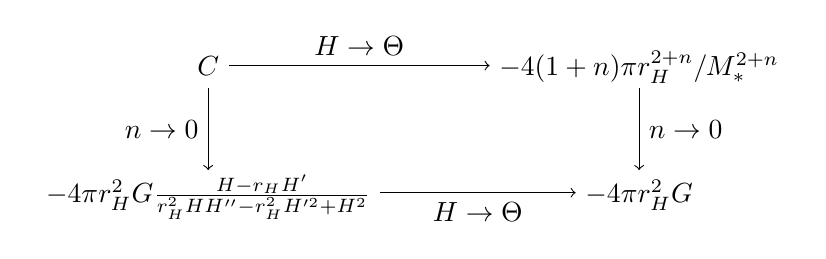
\begin{tikzpicture}[baseline=-0.8ex]
    \matrix (m) [
            matrix of math nodes,
            row sep=3em,
            column sep=4em,
            text height=1.9ex, text depth=0.25ex
            ] {
        C      & - 4(1+n)\pi r_H^{2+n} / M_*^{2+n}   \\
        - 4\pi r_H^2 G \frac{H - r_H H'}{r_H^2 H H'' - r_H^2 H'^2 + H^2}         & -4\pi r_H^2 G \\
        };
    \path[->]
        (m-1-1) edge node[above] {$H\to \Theta$} (m-1-2)
        (m-1-1) edge node[left]  {$n \to 0$} (m-2-1)
        (m-1-2) edge node[right] {$n \to 0$} (m-2-2)
        (m-2-1) edge node[below] {$H \to \Theta$} (m-2-2);
\end{tikzpicture}   
\end{equation}
Depending on $H(r)$, the heat capacity possibly undertakes changes of sign, where a phase transition takes place ($C\to\pm\infty$). Radii here $C(r)\to\pm\infty$ are called critical radii and labeled $r_C$. At such a point, the black hole temperature $T_H(r_C)$ (eq. \ref{eq:T-for-H}) is maximal:

\begin{equation}\label{eq:rc-generic-H}
\left. \partial_{r_H} T_H \right|_{r_H=r_C}=0
\Leftrightarrow
r_C = \sqrt{\frac{1+n}{H'(r_C) - H''(r_C) H(r_C)}} H(r_C).
\end{equation}
As $H(r)\to\Theta(r)$, the critical point goes to zero. This corresponds to the fact that the Schwarzschild metric has no critical point.

\subsection{Entropy}
Entropy is a measure of information, and there are many definitions for it. In statistical mechanics, entropy is typically defined as the amount of ignorance of information of a physical state of a thermodynamical system. It therefore counts all micro states which define an emerging macroscopic state.

In the context of black holes, entropy is maybe the most interesting quantity, since it deals with the \emph{information paradox} of black holes. It is the issue what happens with information (i.e. physical states) that crosses the event horizon.

The Hawking-Bekenstein entropy is defined via the Hawking Temperature $T_H$ as
\begin{equation}
S = \int \frac{\d M}{T_H}.
\end{equation}

The entropy defining integral can also be subsituted like in the heat capacity in the section before, giving for generic $H$ a compact expression:
%
\begin{equation}\label{eq:generic-entropy-integral}
\highlight{
S(r) = \int \frac{\d M}T = \int
\d r_H \left(\frac 1T  \dd M{r_H} \right)
= \frac{\pi (n+2)}2 M_*^{n+2} \int \d r_H \frac{r_H^{1+n}}{H(r_H)}
}
\end{equation}
Approaching the limit $H\to\Theta$, one gets the Entropy of the Schwarzschild-Tangherlini black hole,
\begin{equation}
\frac{\pi (n+2)}2 M_*^{n+2}  \int \d r_H ~r_H^{1+n}
= \frac{\pi (n+2)}{2(n+1)} M_*^{n+2}  r_H^{2+n}.
\end{equation}
Taking the limit $n\to 0$, one gets the Hawking-Bekenstein entropy for the four dimensional Schwarzschild black hole
\begin{equation}
\pi M_*^{n+2} r_H^2
=
\frac{\Omega_2 r_H^2}{4 G}
\,,\quad
\text{with}~~\Omega_2 = 4\pi
\end{equation}

%\todo[inline,color=blue!30]{{\bf Answer} to your comment considering the Entropy $S$: {\it From NCBH I got the gamma, this sounds to be wrong}, according to the $1/H(r_H)$ in the denominator of \eqref{eq:generic-entropy-integral}:
%\\ {\bf I pressume my result is right}. I might insert a chapter discussing GUP and NCBHs in a short as candidates for $H(r)$. I then
% expect $H(r) \sim \gamma\left(\frac 32, \frac {r^2}{4\theta}\right)$ according to eq. (61) in your 2008 NCBH review \cite{N2008NCBH}
%\url{http://arxiv.org/abs/arXiv:0807.1939}.}

\section{Nonlocal operator}\label{sec:H-nonlocal-op}

In this chapter, I want to derive a nonlocal operator $\C A^{-2}(\bv x)$ for the given smearing models $H(r)$. In the long distance limit (where the fundamental length $L_*$ can be considered zero: $L_*/r\to 0$), this operator is supposed to vanish $\C A^{-2} \to 1$. This section ties up with the introduction of nonlocal operators given in the previous chapter according to \cite{NFeb2012,MMN2010}.

The operator is linked to $H(r)$ with a Fourier transformation. It is important to remember that Fourier transformations do not exist in curved space. In the present case, it is possible to define the Fourier transformation in the coordinate frame of the freely falling observer. Therefore it is possible to compute the inverse $\C A^2$ of $\C A^{-2}$ by working in momentum space.

Linking $H(r)$ to the nonlocal operator can be done with the two representations of $\C T^0_0$ that were presented in the text. The smeared energy-momentum tensor of the point-mass reads
\begin{equation} \label{eq:mee-T00-CA}
\C T_0^0 = M \C A^{-2}(\square) \delta^{3+n}(\vec x).
\end{equation}
It is supposed to produce the matter density given in \eqref{eq:rho-H-ndim},
%
% see
% http://tex.stackexchange.com/questions/67651/repeating-an-equation-and-getting-the-same-equation-number
% um die alte Formel nochmal "auszugraben"
%
\begin{equation} \label{eq:mee-T00-classic}
\C T_0^0 = \frac{M}{\Omega_{n+2} ~r^{n+2}} \dd{H(r)}r.
\end{equation}
Matching equations \eqref{eq:mee-T00-CA} and \eqref{eq:mee-T00-classic} means
\begin{subequations}
\begin{equation}
\highlight{
\CA^{-2}(\square)\delta^{3+n}(\vec x)  = \frac 1{\Omega_{n+2} r^{n+2}} \dd{H(r)}r
}%eoh
\,.
\end{equation}
%\intertext{
Writing the Dirac delta by its plane wave momentum space representation $\delta(\vec x)=\int \d^{3+n} p~e^{+ipx}$ on the left hand side and inserting a $1=\C F^{-1} \C F$ by means of a double Fourier transformation on the right hand side allows computing a solution for the operator in momentum space by means of a Fourier transformation of the right hand side:
\begin{align}
\Leftrightarrow  \int \d p^{3+n}~ \CA^{-2}(\square)~e^{ipx} &= 
\frac 1{\Omega_{n+2} r^{n+2}} \dd{H(x)}x
\\
\Leftrightarrow \int \d^{3+n} p~ \CA^{-2}(p^2)~e^{ipx}
&= \int \d^{3+n} p~ 
\overbrace{
\left(
\frac{1}{(2\pi)^{2+n}}
\int \d^{3+n} z
\frac 1{\Omega_{n+2} {\|z\|}^{n+2}}
\dd{H(\|z\|)}{\|z\|}
e^{-ipz}
\right)
}^{ \tilde{T}^0_0(p) }
e^{ipx}
\\
\label{eq:A2-def-by-H}
\Leftrightarrow  \CA^{-2}(p^2) &= 
\frac{1}{(2\pi)^{2+n} \Omega_{n+2}}
\int \d^{3+n} z
\frac 1{z^{n+2}} \dd{H(z)}{z}
e^{-ipz}
\end{align}
\end{subequations}

Note that, by concept, the operator $\C A^{-2}$ is dimensionless. It is therefore valid to switch the coordinate system $(r,p)\to(z,q)$ without prefactors, where $z=r/L_*$, $q=p L_*$ are dimensionless coordinates with the fundamental length scale $L_*$.

\subsection{Higher-dimensional Fourier Transformation}\label{sec:hd-ft}
To solve \eqref{eq:A2-def-by-H}, one can integrate out all extra dimensional angles and effectively reduce the higher-dimensional fourier transformation of the radial symmetric function to a one dimensional one. Calling $V(r) := \frac{H'(r)}{r^{n+2}}$ the higher dimensional Fourier kernel, an effective one-dimensional Fourier transformation is be derived in this section. This is motivated by the well-known three dimensional procedure which is easier to read and given in appendix \ref{appendix:fourier1}.

Start with the $N=n+3$-dimensional fourier transformation and rewrite it into conventional polar coordinates:
\begin{subequations}
\begin{align}
\hat V(p) &= \frac{1}{(2\pi)^{3+n}} \int \d^{3+n} r~e^{-i \vec r \cdot \vec p} V(r)
\\
&= \frac{1}{(2\pi)^{3+n}} \int_0^\infty \d r~r^{2+n} \int_0^{2\pi} \d \varphi
\prod_{i=1}^{n+1} \int_0^\pi \d \theta_i \sin^i(\theta_i)~e^{-i \vec r \cdot \vec p} V(r)
\intertext{Now use the angle $\theta_1$ for identification with the inner scalar product angle $\vec r \cdot \vec p := rp \cos\theta_0$. Subsitute $\int_0^\pi  \d \theta_1 \sin(\theta_1) = -\int_{-1}^{+1} \d \cos \theta := \int_{-1}^1 \d x$. Integrating out \emph{all other} $n$ angles $\theta_i$ as well as the angle $\varphi$ gives a $\Omega_{2+n}/2$ contribution, as the $n+3$-sphere volume is given by $\int \d^{3+n} r = \int \d r\Omega_{n+2} r^{n+2}$. Divide it by the missing factor $\int_0^\pi \d \theta \sin(\theta)=2$, used for the scalar product substitution. One ends up with
}
&=
\frac{1}{(2\pi)^{3+n}} \frac{\Omega_{n+2}}{2} \int_{-1}^{+1} \d x \int_0^\infty \d r~r^{2+n} V(r)~e^{-irpx}
\\
&= \frac{1}{(2\pi)^{3+n}} \frac{\Omega_{n+2}}{2} \int_0^\infty \d r~r^{2+n} V(r)
   \left[ \frac{1}{-ipr} e^{-iprx} \right]^{+1}_{-1}
\\ \label{eq:ftN-split-int}
&= \frac{1}{(2\pi)^{3+n}} \frac{\Omega_{n+2}}{2} \frac{i}{p}
\left(
\int_0^\infty \d r~r^{1+n} V(r) e^{-ipr} -
\int_0^\infty \d r~r^{1+n} V(r) e^{+ipr} \right)
\intertext{To write this line as an effective one dimensional Fourier transformation, transform the second integral in line \eqref{eq:ftN-split-int}, first by switching the integral borders, $\int_0^\infty \d r = \redmin \int_\infty^o \d r$, second by variable substitution $r := \redmin r'$. This inserts an alternating minus, depending on $n$, as $r^{1+n}\d r=(\redmin 1)^{1+n} (r')^{1+n} (\redmin 1)\d r' = (\redmin 1)^n r'\d r'$. Note the substitution also toggles the sign of the integral borders, allowing to combine both integrals to
}
&= \label{eq:ftN-result-theta}
\frac{1}{(2\pi)^{3+n}} \frac{\Omega_{n+2}}{2} \frac{i}{p}
\int_{-\infty}^{\infty} \d r~r^{1+n}
\left[ V(r) \Theta(r) + (-1)^n V(-r) \Theta(-r) \right] e^{-ipr}
\\
&= \frac{1}{2 \pi} \int_{-\infty}^\infty \d r~v(r)~e^{-ipr}.
\end{align}
\end{subequations}
One derives an effective one dimensional Fourier transformation of the effective function
\begin{equation}
v(r) :=
\frac{1}{(2\pi)^{2+n}} \frac{\Omega_{2+n}}2 \frac{i}{p} r^{1+n} \left[ V(r) \Theta(r) + (-1)^n V(-r) \Theta(-r) \right].
\end{equation}
Note that the Heaviside step function $\Theta(z)$, which was used to combine the integrals from line \eqref{eq:ftN-split-int} to one in \eqref{eq:ftN-result-theta} is understood on the complex plane as
\begin{equation}\label{eq:hd-ft-req-theta}
\Theta(z) = \Theta(\Re z).
\end{equation}
The requirement \eqref{eq:hd-ft-req-theta} must be only exactly fulfilled at the evaluation points of the integral, that is, the poles of $v(r)$. This is a weaker requirement for $\Theta(z)$ on the complex plane:
\begin{equation}\label{eq:hd-ft-weak-theta}
\Theta(z) =
\begin{cases}
\Theta(\Re z) \quad &\text{if}~ z~\text{is a pole of } v(r), \\
\text{arbitrary finite value} \quad & \text{else}.
\end{cases}
\end{equation}
See appendix \ref{appendix:fourier} for a proposed function fulfilling \eqref{eq:hd-ft-weak-theta}.

Issues may arise with holomorphy when Cauchy theorem is applied. This is also discussed further in the appendix \ref{appendix:fourier}, realizing that solving the integral on the complex plane works in three dimensions, so it shall work in any higher number of dimensions. Note that this approach was also successfully applied to a GUP-inspired nonlocal operator in an onging work \cite{Knipfer2014}.

\subsection{Inverting the bilocal smearing operator}
It is possible to solve the $\C A^{-2}$ integral \eqref{eq:A2-def-by-H} by rewriting it to an one-dimensional one. By inserting
\begin{equation} \label{eq:generic-bigV}
V(r) = \frac{1}{\Omega_{n+2} r^{n+2}} \dd{H(r)}{r}
\end{equation}
into equation \eqref{eq:ftN-result-theta}, a compact integral can be derived:
\begin{equation} \label{eq:A2-def-one-dimension-integration}
\highlight{
\C A^{-2}(p^2) =
\frac{1}{(2\pi)^{3+n}} \frac{i}{2p}
\int_{-\infty}^\infty \d r \frac{H'(|r|)}r e^{-ipr}.
}%eoh
\end{equation}
This equation can be solved with the residue theorem. Since in \eqref{eq:A2-def-one-dimension-integration}, $r\equiv\|\vec r\| \geq 0$ and $p\equiv \|\vec p\| \geq 0$, there is only one integration contour for Jordan's lemma. For the forward Fourier transformation $\C F_1$, as seen in \eqref{eq:A2-def-one-dimension-integration}, the contour is determined by requiring (for some constant $\# > 0$ representing the momentum)
\begin{equation} \label{eq:jordan}
\lim_{r\to \pm i \infty} e^{-ipr} = 0
~\Rightarrow~
e^{-i (+\#) (\pm i\infty)} = e^{\pm \infty \#} = 0
~\Rightarrow~
r \to -i\infty,
\end{equation}
i.e. it is closed on the lower half complex plane ($\Im r < 0$). For the inverse Fourier transformation $\C F_1^{-1}$, it is closed on the upper half complex plane ($p \to i\infty \Leftrightarrow \Im p > 0$). 

Concluding, equation \eqref{eq:A2-def-one-dimension-integration} allows deriving the inverse bilocal operator by inserting a specific choice of $H(r)$.


\chapter{The holographic black hole in higher dimensions} \label{sec:holo}
In this chapter, a member of the black hole family discussed in the previous chapter is proposed. It is based on a black hole proposed in \cite{NS2013}. It tackles the problems of the Schwarzschild black hole presented in the previous chapters. It will be derived that the class of black holes proposed in this chapter features:
\begin{enumerate}
\item A modified short-distance behaviour which allows the physical system to arrive at a \emph{cold evaporation endpoint} (black hole remnant), supported by regular thermodynamics.
%
\item A \emph{classical low-energy limit}, that is, Schwarzschild behaviour of the metric for big distances, in terms
\begin{equation}
g_{00}(r) = 1 - \frac{2GM}{r} \quad \text{for} \quad r \gtrsim l_0.
\end{equation}
%
\item \emph{Self-encoding} of the characteristic minimal length scale $l_0$ in the radius of the \emph{extremal} configuration $r_0$, that is,
\begin{equation}\label{eq:self-encoding-principle}
l_0 = r_0.
\end{equation}
%
\item \emph{Logarithmic entropy corrections}, like most theories of quantum gravity propose.
%
\item Compatibility with \emph{large extra dimensions}: All previous points can be implemented in the ADD scenario, and one may identify the length scale $l_0$ with the fundamental length $L_*$.
\end{enumerate}
It will be shown that this class of black holes still possesses a curvature singularity at the origin ($\lim_{r\to 0} R = \infty$). Anyway the property of self-encoding is crucial: It enables $l_0$ being the only \emph{universal scale}, as the theory requires no new length scale like $\sqrt{\beta}$ from GUP, $\theta$ from NCG or $\ell_0$ from String Theory.

This class of black holes is implemented by a special choice of $H(r)$ that will be refered to as $h(r)$ for distinction. By inserting $H(r)=h(r)$ in any equation of chapter \ref{sec:generic-H}, a number of physical properties will be derived in this chapter. $h(r)$ defines the \emph{holographic black hole} in $n$ large extra dimensions:
\begin{equation}\label{eq:holo-def-maintext}
h(r) := \frac{r^{2+n}}{r^{2+n} + \tilde r^{2+n}_0}.
\end{equation}
$\tilde r_0$ is a regulation constant of dimension length that is discussed in the next sections. For $n\to 0$, the profile \eqref{eq:holo-def-maintext} reduces to the four dimensional profile first studied by Nicolini and Spalluci in \cite{NS2013}.


\begin{figure}[b!]
\centering
\begin{subfigure}{0.5\textwidth}
\caption{Heaviside approximation $h(r)$}
\label{fig:profile-h}%
\includegraphics[width=\textwidth]{figures/profile-h.pdf}
\end{subfigure}%
\begin{subfigure}{0.5\textwidth}
\caption{Dirac-delta approximation $h'(r)$}
\label{fig:apx-dirac-h}%
\includegraphics[width=\textwidth]{figures/dirac-profile-h.pdf}
\end{subfigure}%
\caption[Plots of the holographic function $h(r)$ and its derivative.]{The Heaviside (a) and Dirac delta (b) approximation profile $h(r)$ against its built in length scale $\tilde r_0$ for a different number of large extra dimensions $n$. One sees that $\tilde r_0$ plays the role of the \emph{width} of the profile. By choice, it is a kind of ``half-life scale'', as can be computed when computing $h(\tilde r_0)=\nicefrac 12$. Note also that increasing $n$ create sharper distributions. For $n\to \infty$, the curve resembles a displaced step function $h_{n\to\infty}(r)=\Theta(r-\tilde r_0)$. This reflects the fact that all volume in a $\infty$-sphere lives on the surface.}\label{fig:profiles-h}
\end{figure}

Inserting $h(r)$ into the generic gravitational potential \eqref{eq:V-for-generic-H} creates for a fixed $n$ and $\tilde r_0$ a geometry, uniquly determined by its mass $M$:
\begin{equation}\label{eq:V-for-holo}
V(r) = \frac{1}{2+n} \frac{M}{M_*^{n+2}} \frac{r}{r^{2+n} + \tilde r_0^{2+n}}.
\end{equation}
The gravitational potential \eqref{eq:V-for-holo} spawns a class of black hole geometries which is subject of this chapter.

Note that this profile is an \emph{ab-initio} proposal, and especially the higher dimensional continuation is ``guessed''. The special feature is that \emph{there is no further ingredient than general relativity}. There is no need to stress a more advanced theory like String Theory or loop quantum theory to generate the metric defined by \eqref{eq:V-for-holo}.

Compared to \cite{NS2013}, the holographic metric was extended to higher dimensions. The higher dimensional modification will be justified by yielding logarithmic corrections to the black hole entropy in any number of dimensions.

\section{Geometry}\label{sec:geometry-holo}
\subsection{Horizons}
The event horizon equation, considering $r_H$ being the event horizon, requires
\begin{equation}
0 = g_{00}(r_H)
\quad\Rightarrow\quad
0
= z^{2+n} - z\, m_n + 1,
\quad\text{with}~~ m_n = \frac 1{n+2} \frac M{M_*^{n+2}}
\end{equation}
and $z=r/\tilde r_0$. The number of (physically meaningful) solutions depends on $m_n$, that is, on the black hole mass $M$. For any $n$, there are three possible solutions, plotted in figure~\ref{fig:g00-holo}. They are distinguished by the value of the ratio $M/M_0$, with the extremal mass $M_0$ that is found to be a special value:

\begin{description}
\item[$M < M_0$]
The mass is too small to create a black hole. The physical object is a vacuum, self-gravitating particle-like structure which is stable.

\item[$M > M_0$] There are two horizons with radii $r_\pm$. In figure \ref{fig:g00-holo}, they are indicated by red dots. Physically, one can argue that the outer horizon $r_+$ is the more relevant one, since it \emph{shields} the black hole inner structure. Mathematically, $r_-$ is a Cauchy horizon, and in the region $r_- < r < r_+$, where $g_{00}>0$ and $g_{rr}<0$, the coordinates $r$ and $t$ switch their meaning (cf. section \ref{sec:conformal}).

There are no meaningful compact analytic expressions for the values of $r_\pm$, expcept for the holographic metric and without extra dimensions ($n=0$), as already given in \cite{NS2013}:
\begin{equation}
r_\pm = GM \pm \sqrt{G M^2 - 4}.
\end{equation}
For $n>0$ and especially for the self-regular metric, the roots of \eqref{eq:horizons} can simply be determined numerically. %The values of $r_+$ are given in table \ref{table:Length-scales}.

Note that for $M \gg M_0$, $r_+$ approaches the Schwarzschild-Tangherlini horizon.

\item[$M = M_0$]
The two horizons merge to a single horizon which is called \emph{extremal} or \emph{degenerate} horizon $r_\pm = r_0$ and identified with the extremal mass $M=M_0$. In figure \ref{fig:g00-holo}, the green line displays the coefficient $g_{00}$ with extremal mass, showing a single horizon, indicated by the green dot. Figure \ref{fig:g00-holo-higher-n} displays the extremal configuration in higher dimensions.
\end{description}
%

\begin{figure}
\begin{subfigure}{\textwidth}
\caption{$g_{00}$ in $n=0$ for different masses $M$.}\label{fig:g00-holo}
\includegraphics[scale=1]{figures/remnant-plot-holography.pdf}
\end{subfigure}
\begin{subfigure}{\textwidth}
\caption{$g_{00}$ for $M=M_*$ in different dimensions $n$.}\label{fig:g00-holo-higher-n}
\includegraphics[scale=1]{figures/remnant-plot-holography-n.pdf}
\end{subfigure}
\caption[Plots of the $g_{00}$ component of the holographic black hole.]{The holographic gravitational potential. The upper panel \ref{fig:g00-holo} shows different geometries based on the black hole mass. The three curves represent a smaller than critical-mass (blue), critical mass (green) and heaviest mass (red).

The lower panel \ref{fig:g00-holo-higher-n} shows the higher dimensional extension for the self-encoding masses $M_0=M_*$. All curves are scaled for the individual $L_*$ according to the numerical values given in table \ref{table:critical-r}.

Compared to the fourdimensional metric (fig. \ref{fig:g00-holo}), one can see that the picture basically \emph{stays the same}. In this figure, the curves qualitatively get ``sharper'' with increasing $n$, which corresponds to the increasing surface to volume ratio of $n$-spheres, which is a purely geometrical effect.

In any case, the dashed lines correspond to the equivalent Schwarzschild metric.}
\end{figure}

\clearpage
\subsection{The self-encoding remnant}
In the present class of black hole geometries, the extremal black hole configuration parameter $M=M_0$ or $r=r_0$ can be \emph{self-encoded} with the built-in length scale $\tilde r_0$. The relation is found by inserting $h(r)$ into the second remnant equation \eqref{eq:remnant-H-eq2}:%. This yields
%
\begin{equation}\label{eq:r0-holo}
\highlight{r_0 = \tilde r_0~\left( \frac 1{1+n} \right)^{\frac 1{2+n}}}
\end{equation}
%
Equation \eqref{eq:r0-holo} allows to connect the length scale $\tilde r_0$ introduced as ``built in'' length scale in the holographic profile to a physical length scale $r_0$. This equation can be used to eliminate $\tilde r_0$ from the holographic profile \eqref{eq:holo-def-maintext} in favour of the physical meaningful $r_0$:
\begin{equation}\label{eq:holo-transform1}
h(r) = \frac{r^{2+n}}{r^{2+n} + \tilde r_0^{2+n}}
= \frac{r^{2+n}}{r^{2+n} + (1+n) r_0^{2+n}}.
\end{equation}

Note that the \emph{self-encoding} principle requires that the size of the remnant $r_0$ should be identical to the fundamental length scale of the physical theory $l_0$. For gravity in 4d space time, the only fundamental length scale is given by the coupling constant (Newtons constant) $G$ which defines the Planck length $L_\text{Pl} = \sqrt{G} \approx 10^{-35}\,$m. In 4d, \eqref{eq:r0-holo} assures this is true, as already stated in \cite{NS2013}:
\begin{equation}
r_0 \musteq l_0 = L_\text{Pl} = \tilde r_0.
\end{equation}
%
With extra dimensions, there is the reduced Planck length $L_*$ which is the actual fundamental length scale $l_0$, since the observable Planck length $L_\text{Pl}$ is just a large-distance effective one. To express $h(r)$ only in terms of $L_*$, require $r_0 \musteq l_0 \equiv L_*$ and find
%
\begin{equation}
\label{eq:rtilde0-holo}
\tilde r_0 = (1+n)^{\frac 1{2+n}}~L_* \,.
\end{equation}
%
Implementing the self-encoding value for $\tilde r_0$ into the holographic profile \eqref{eq:holo-transform1} gives a profile which contains nothing more than the universal physical constant $L_*$:
\begin{equation}\label{eq:holo-without-rtilde}
h(r) = \frac{r^{2+n}}{r^{2+n} + (1+n) L_*^{2+n}}
\end{equation}

When computing $M_0=M(r_0)$, the self-encoding of the fundamental mass scale $M_*$ is expected, that is, $M(r_0) = M_*$. It is $h(L_*) = 1/(2+n)$ and thus, by construction,
\begin{equation}
M(L_*) = \frac{1}{n+2} \left( \frac{L_*}{L_*} \right)^{1+n} \frac{1}{h(L_*)} M_* =  M_*.
\end{equation}
%

\begin{table}
\begin{tabularx}{\linewidth}{ l X }
\firsthline
symbol & meaning \\
\hline
$r$   & A placeholder for a radius. \\
$r_H$ & The black hole horizon radius. \\
$r_+$ & The outer Cauchy horizon of the holographic black hole, this is (if applicable) always accessible. \\
$r_-$ & The inner Cauchy horizon of the holographic black hole, it is not visible from outside. \\
$r_0$ & The extremal black hole horizon radius. When $r_+ = r_-$, the symbol $r_0$ is used. \\
$r_C$ & The critical radius, at this radius the temperatures are maximal. \\
$L_*$  & The fundamental length in the ADD scenario. In this chapter it is the fundamental physical length. \\
$\beta$ & The fundamental length in the GUP scenario. \\
$\theta$ & The fundamental length in the NCBH scenario. \\
$L_\text{Pl}$ & The Planck length (fundamental length in classical GR). \\
$l_0$ & A placeholder for a fundamental physical length scale. Possible values are e.g. $l_0\in \{L_*, L_\text{Pl}, \beta, \theta, \dots \}$. \\
\hline
\end{tabularx}
\caption[Overview table for length variables like $r_H, r_0, r_C, L_*, l_0, \dots$]{Variables representing lengths used in this chapter. According to Mass=$1/$Length, each length scale represents also a mass scale.}
\end{table}

\begin{figure}
\centering
\begin{subfigure}{0.45\textwidth}
\caption{BH--particle duality in $n$ LXDs}\label{fig:bh-duality-STM-revisited}
\includegraphics[width=\textwidth]{figures/completeness-STM.pdf}
\end{subfigure}%
\hspace{0.03\textwidth}
\begin{subfigure}{0.45\textwidth}
\caption{Holographic BH in $n$ LXDs}\label{fig:bh-duality-holo-B}
\includegraphics[width=\textwidth]{figures/completeness-holoN.pdf}
\end{subfigure}
\caption[Length scales for the holographic black hole in higher dimensions.]{The holographic black hole (right panel) solves the BH--particle duality problem, shown in the left panel (it is figure \ref{fig:bh-duality-SS} from section \ref{sec:bh-particle-duality}).}\label{fig:completeness-holoN}
% Wo es noch nur ein Bild war (Text neben Bild):
%
%\floatbox[\capbeside\thisfloatsetup{floatwidth=\textwidth,capbesidewidth=sidefil,capbesideposition={right,top}}]{figure}[\FBwidth]{%
%\caption[TODO {\bf PENDING} TEXT HERE]{The two horizons of the holographic black hole stand out in this plot as the upper and lower branches of the blue curves. While the upper branch represents the 
%}
%}{\includegraphics[width=8cm]{figures/completeness-holoN.pdf}}
\end{figure}

\subsection{Minimal length}
Figure \ref{fig:completeness-holoN} shows how the holographic black hole prohibits physics below the Planck scale by implementing the self-completeness principle. The quantum mechanics regime ($M<M_*$) and the general relativity regime ($M>M_*$) are clearly separated, and the holographic black hole never accesses the sub-Planckian regime but instead builds out a remnant (black dot).

Considering the right panel, the two horizons of the holographic black hole stand out as the upper and lower branches of the blue curves.  While the upper branches display $r_+ > L_*$, the ``visible'' event horizons, the lower branches display the cauchy horizons $r_- < L_*$ that are shielded by $r_+$ for big masses $M > M_*$ and non-accessible by the remnant at $M=M_*$.

\subsection{Curvature singularity}
According to the curvature considerations for general profiles $H(r)$ in section \ref{sec:general-curvature}, the holographic metric is still diverging.
%
One can give an estimation for $R(0)$ based on the taylor expansions of the holographic profile $h(r)$ at $r=0$:
\begin{equation}
h(r) = \left( \nicefrac r{L_*} \right)^{2+n} + \C O\left( \left( \nicefrac r{L_*} \right)^{2 (2+n)}\right), h'(r) \approx \left( \nicefrac r{L_*} \right)^{1+n}, h''(r) \approx \left( \nicefrac r{L_*} \right)^n
\end{equation}

Inserting this into $R(r)$ for $H(r)$, equation \eqref{eq:R-for-H}, gives $H(0)\approx {L_*}/r$. The holographic black hole has therefore still a curvature singularity at the origin.

\vfill
\begin{table}[h!]
\begin{center}
\begin{tabular}{lcccccccc}
\firsthline
 $n$ & 0 & 1 & 2 & 3 & 4 & 5 & 6 & 7 \\
   \hline
 $\tilde r_0$ & 1.00 & 0.79 & 0.76 & 0.76 & 0.76 & 0.77 & 0.78 & 0.79 \\
 $r_C$ & 2.06 & 1.60 & 1.48 & 1.41 & 1.36 & 1.33 & 1.30
   & 1.28 \\
 $T(r_C)$ & 0.024 & 0.07 & 0.12 & 0.18 & 0.25 & 0.31 & 0.38 & 0.44 \\
   \hline
\end{tabular}
\end{center}
\caption[Numerical values for the holographic black hole critical radii, Temperatures, etc.]{Numerical properties of the holographic black hole. All values are given in $n$d Planck units (as multiples of $L_*$). $\tilde r_0$ is the initial length scale of $h(r)$ that was used to fix the self-encoding of the theory, according to eq. \eqref{eq:r0-holo}. Going from eq. \eqref{eq:holo-def-maintext} to \eqref{eq:holo-without-rtilde}, $\tilde r_0$ could be eliminated in favour of the fundamental $L_*$.

$r_C$ is the critical radius according to eq. \eqref{eq:rc-holo}. $T(r_C)$ is the Hawking temperature for a black hole with extend $r_C$, it is the maximum temperature, also indicated in figure \ref{fig:T-holo}.
}\label{table:critical-r}
\end{table}

\clearpage
\section{Thermodynamics}\label{sec:holo-thermodynamics}
The thermodynamics of the holographic black hole arise from the equations given in section \ref{sec:general-thermo}. By inserting the holographic profile $h(r)$ in the equations derived for general $H(r)$, the quantities in this section are derived.

Note that in this section, $r_H$ always represents the outer horizon $r_+ > L_*$ which is the physical meaningful horizon for calculating thermodynamics of the holographic black hole.

\subsection{Hawking Temperature}
The Hawking Temperature of a holographic black hole with radius $r_H$ in $n$ LXDs is determined by \eqref{eq:T-for-H} to
%
\begin{equation}
T_H = \frac{1}{4\pi r_H}
\left(
1 + n - (2+n)
\frac{(L_*/r)^{(2+n)}}{1+(L_*/r)^{(2+n)}}
\right).
\end{equation}

Figure \ref{fig:T-holo} shows the temperature of the black holes. Comparing with the appropriate Schwarz\-schild black hole in $n$ dimensions, the first thing to be noticed is the difference of the two curves which becomes large below $r \lesssim 3L_*$ or $r \lesssim \nicefrac 32 r_C$, with the critical temperature $r_C$ as defined in the next section. There is a maximum temperature at the critical radius $r_C$ (indicated by the dots in fig. \ref{fig:T-holo}, numerical values are given in table \ref{table:critical-r}), and for smaller radius the black hole cools down until it reaches zero temperature at $r_0$. One therefore speaks of a \emph{cold} remnant. 

\begin{figure}[h!]
\includegraphics[scale=1]{figures/temperature-plot-holography-n.pdf}
\caption[Holographic metric temperature plot]{Temperature of the holographic black hole, compared to the dashed-line Schwarzschild-Tangherlini black hole temperature, in a different number of dimensions. The circles indicate the critical radii (eq. \ref{eq:rc-holo}) where maximal temperatures occur.}\label{fig:T-holo}
\end{figure}

The maximum temperature $T(r_C)$ is also the upper bound to argue about the validity of the theory. As at any point $r$, $T_H(r)/M < T_H(r_C)/M_* < 1$, backreaction effects can be neglected \cite{NS2013}. Considering the numerical values (c.f. table \ref{table:critical-r}), the situation gets worse for higher dimensions $n$, as backreaction effects compared to the fundamental Planck scale get more and more important.

\subsection{Heat capacity}
The heat capacity of a holographic black hole with radius $r_H$ in $n$ LXDs is determined by \ref{eq:C-for-H} to
\begin{equation}
C = - \frac{4\pi r_H^{2+n}}{M_*^{n+2}}
\frac{ \left(r_H^{-n} + r_H^2\right)^2 \left( (1+n) r_H^2 - r_H^{-n} \right)}
{ \left( 4 + 3n + n^2 \right) r_H^{n-4} + r_H^{2n-2} - (1+n)r_H^6}
\,.
\end{equation}
%
The critical radius can be determined by evaluating the extremal temperature condition and inserting the current black hole model into \eqref{eq:rc-generic-H}:
%
\begin{equation}\label{eq:rc-holo}
r_C = 2^{\frac{1}{n+2}} \left((2+n) \sqrt{n^2+2 n+5}
-n^2+3 n-4\right)^{-\frac{1}{n+2}} ~L_*
\end{equation}

\begin{figure}
\begin{center}
\begin{subfigure}{\textwidth}
\caption{Heat capacity $C$ for different $n$, scaled against individual $L_*$}
\includegraphics[scale=1]{figures/heat-capacity-plot-naive-holography-n.pdf}
\end{subfigure}
\begin{subfigure}{\textwidth}
\caption{Heat capacity $C$ for different $n$, scaled against $L_*$ and shifted around $r_C$}
\includegraphics[scale=1]{figures/heat-capacity-plot-holography-n.pdf}
\end{subfigure}
\end{center}
\caption[Holographic metric heat capacity plots]{The heat capacity of the holographic black hole for different extra dimensions $n$, as a function of the black hole size $r_H$. The dashed line corresponds to the heat capacity of the classical Hawking-Beckenstein black hole in $n$ extra dimensions.}
\end{figure}

\subsection{A phase transition}\label{sec:phase-transition}
Eventually, having computed $g_{00}, T$ and $C$, one is able to compare those quantities for black hole stability discussion. Figure \ref{fig:thermodynamic-comparison} illustrates the curves and different phases, exemplary for the holographic black hole. Considering the sign of the heat capacity, three phases can be distinguished:

\begin{description}
\item[$r > r_C$ .] The heat capacity is negative, the system is instable: Losing mass by radiation makes it hotter and hotter. This behaviour is well described by the Schwarzschild metric.

When reaching $r \to^+ r_C$, in the modified metrics this process stagnates, the temperature no longer rises. Now a phase transition takes place at $r_C$, the system gets stable.

\item[$r_0 < r < r_C$ .] The heat capacity is positive and the black hole system is stable. Losing mass now results in losing temperature. The system heavily deviates from the classical Schwarzschild solution. The Temperature decreases until it evventually reaches zero.

\item[$r < r_0$ .] This phase is physically never accessed, as the system got stable at $r_0$. The self-complete paradigm also ensures that no black holes cannot be generated at these distances, as smaller length scales then $r_0$ are not accessible.

Thermodynamics in this area is not physically meaningful. Mathematically, there is a negative temperature $T < 0$ and the system is basically instable again, since $C < 0$.
\end{description}

\begin{figure}
% trim=l b r t, use \fbox{} around includegraphics to view.
\makebox[\textwidth][c]{\includegraphics[scale=1,trim=2cm 0 1cm 0,clip=true]{figures/thermodynamic-big-plot.pdf}}
\caption[Three panel plot: Temperature, heat capacity and entropy]{Comparison of temperature (top panel), heat capacity (middle panel) and entropy (bottom panel) on the same scale (Planck units everywhere). Here, $n=2$, but the plot looks systematically the same in all dimensions. The dashed curves are the corresponding Schwarzschild behaviour.

Regarding the sign of the heat capacity (Sign $C=\pm 1$), there are three different states, indicated by colors and seperated by $r_0$ (blue line) and $r_C$ (red line). Blue circles indicate the final, cold and stable evaporation state. The red circle indicates the position of the critical radius. Note that the shaded region $r_H<L_*$ is physically not accessible and in the self-complete paradigm of general relativity, thermodynamics are not defined there.
}\label{fig:thermodynamic-comparison}
\end{figure}

\subsection{Entropy}\label{sec:holo-entropy}
Inserting the holographic profile $h(r)$ into the entropy integral \eqref{eq:generic-entropy-integral} gives the entropy of the holographic black hole,
\begin{equation}\label{eq:S-holo-result}
% ziemlich falsch:
%S_h(r) = 4\pi m_n \left( \frac{r^{n+2}}{n+2} + \log(\frac r{L_*}) \right).
S_h(r_H) = \frac{4\pi}{L_*^{n+2}} \left( r_H^{n+2} - L_*^{n+2} \right)
+ 4\pi (n+2) \log \left( \frac {r_H}{L_*} \right)
\end{equation}
Note the \emph{logarithmic quantum corrections}. They motivate the label \emph{holographic} for the metric. The logarithmic term is in aggreement with most quantum gravity theories as string theory and quantum loop gravity (c.f. appendix \ref{sec:apx-qgbhs}).

Since $\log(1)=0$, the entropy goes to exactly to zero for $r_H \to r_0$. The remnant therefore has zero entropy. Physically, this means that there is only one possibilty to realize the remnant. This motivates casting the remnant as a black hole \emph{ground state} and imposing a quantization law.

%If the metric would not scale for higher dimensions, the entropy (for $h(r)=1/(1+(\tilde r_0/r)^2)$ in any $n$) would look like
%\begin{equation}
%S = 4\pi m_n \left( \frac{r^{n+2}}{n+2} + \frac{r^n}{n} \right)
%\quad\text{for } n>0.
%\end{equation}

\begin{figure}[b!]
\floatbox[\capbeside\thisfloatsetup{floatwidth=\textwidth,capbesidewidth=sidefil,capbesideposition={right,top}}]{figure}[\FBwidth]{%
\caption[Artistic illustration of the holographic principle, taken from \cite{kamajian}]{An artistic interpretation of the holographic principle, as it illustrated an science magazine article by Jacob Bekenstein \cite{kamajian}. The black hole entropy is quantizied in terms of Planck units. A Planck area (blue) has $A/4$ units of entropy (red).
}\label{fig:bitsbytes}
}{\includegraphics[width=8cm]{figures/holouniverse03_01.jpg}}
\end{figure}

\subsection{The black hole area quantization picture}\label{sec:holo-area-quant}
The black hole area theorem dates back to Wheeler 1973 and is a recasting of the Schwarzschild black hole entropy in terms of the horizon area $A=4\pi r_H^2$, and therewith
\begin{equation}\label{eq:horizon-byte}
S = \frac A {4A_0}
\quad \text{with}~A_0 = 4\pi L_P^2.
\end{equation}
%
In the same spirit, the holographic metric black hole entropy \eqref{eq:S-holo-result} can be recasted as
\begin{equation}
S_h(A_+) = \frac{\pi}{A_0} (A_+ - A_0) + \pi \log(A_+ / A_0),
\quad\text{with}~~
\begin{aligned}
A_+&=\Omega_{n+2} r_+^{2+n}, \\
A_0&=\Omega_{n+2} L_*^{2+n}.
\end{aligned}
\end{equation}
%
The remnant surface may serve as a ground state for a quantized area spectrum according to the area quantization principles by Dvali \cite{Dvali:2011aa,dvali2}. To do so, any black hole area $A_+$ shall be an integral multiple of $A_0$, in terms
\begin{equation}\label{eq:holo-quant-rule}
A_+ := A_{k-1} = k A_0 = 4\pi k L_*^2,
\quad\text{with}~~k\in\setN.
\end{equation}
Speaking in the language of information theory, the minimal screen $A_0$ may represent the basic information building block, one \emph{byte} \cite{NS2013}. The number $k=1,2,3,\dots$ counts the number of bytes. One can also define one \emph{bit} as the area $L_*^2$ which is the capacity of the smallest reasonable holographic screen according to the completeness principle of GR. According to \eqref{eq:horizon-byte}, four bits make one byte (in computing, this is called a \emph{nibble}). Figure \ref{fig:bitsbytes} displays this principle.

\begin{figure}[b!]
\centering
\begin{subfigure}{0.45\textwidth}
\caption{physical abscissa}\label{fig:mass-quantization-a}
\includegraphics[scale=1]{figures/mass-quantization.pdf}
\end{subfigure}%
\hspace{0.05\textwidth}
\begin{subfigure}{0.45\textwidth}
\caption{abscissa linear in $k$}\label{fig:mass-quantization-b}
\includegraphics[scale=1]{figures/mass-quantization-linear.pdf}
\end{subfigure}%
\caption[Mass quantization plot for the holographic metric]{Mass quantization for different extra dimensions $n$: Figure \ref{fig:mass-quantization-a} basically shows the upper (outer) branch of $M(r_H)$ that was already displayed in figure \ref{fig:bh-duality-holo-B}. The circles represent the discrete masses allowed by quantization rule \eqref{eq:mass-quant-holo}. The circles are filled if $r_H < r_C$, \emph{i.e.} if the BH is in the regime of discrete mass spectra, while unfilled circles display the BH in the more and more continous mass spectrum. Figure \ref{fig:mass-quantization-b} shows the same curves with equidistant discretized radius gap $\Delta r_k = r_k - r_{k-1}$.}
\end{figure}

According to this quantization rule, one can compute the discretized radii, masses and mass gaps. One obtains in $n$ LXDs by inserting \eqref{eq:holo-quant-rule} into \eqref{eq:horizon-byte} and \eqref{eq:Mass-rH}:
\begin{align}
r_{k-1} &= k^{1/(2+n)} L_* \\
\label{eq:mass-quant-holo}
M_{k-1} &= \frac{1}{n+2}\frac{k+1}{ k^\frac{1}{n+2} } M_*
\end{align}
For $n\to0$, this gives the values found in \cite{NS2013}. For $k\gg1$ one finds a continous spectrum of radii and masses. This is supported by the quickly decreasing mass gap for higher states $k$,
\begin{equation}
\Delta M_k := M_k - M_{k-1} 
\xrightarrow{k\to\infty}
\frac{1+n}{(2+n)^2} \frac{1}{k^{1/(2+n)}}
\,.
\end{equation}

As the mass gap quickly decreases, there is a continous mass spectrum for big black holes (big horizon radius $r_H$). In the regime of positive heat capacity $C>0$, due to the big mass gaps, the system can be refered to as a quantum mechanically decaying black hole, while in the regime of negative heat capacity $C<0$, it decays thermally. Therefore, the phase transition from section \ref{sec:phase-transition} separates the semi-classical regime from the quantum system \cite{NS2013}. This behaviour is independent of the number of dimensions $n$.

\section{Modified field equations}\label{sec:modified-einstein}
In the holographic model, insert $h(r)$ to derive from \eqref{eq:A2-def-one-dimension-integration} the expression (note there is no need for powers of $L$ when switching to dimensionless coordinates $z=r/L_*,q=pL_*$)
\begin{equation}\label{eq:A2-holo-def}
\C A^{-2}(q^2) =
\underbrace{\frac{2+n}{(2\pi)^{3+n}} \frac{i}{2q}}_{f_0}
\int_{-\infty}^\infty
\d z
\bigg[
\underbrace{\frac{z^n}{(1+z^{2+n})^2}}_{f_+} \Theta(z)
+
\underbrace{\frac{(-1)(-z)^n}{(1 + (-z)^{2+n})^2}}_{f_-} \Theta(-z)
\bigg]
e^{-i q z}.
\end{equation}
The poles of $f_+$ are the same as for $f_-$, just mirrored at the
imaginary axis $\Re(z)=0$, in symbols $f_+(z)=-f_-(-z)$. The poles of $f_+$ are given by
\begin{equation}
\left( 1 + z^{2+n} \right)^2 = 0
\quad\Leftrightarrow\quad
z = (-1)^{\frac 1{2+n}}
= \exp \left\{ \frac{i\pi + 2\pi ik}{n+2} \right\}
\quad\forall k\in \mathbb{N}_0.
\end{equation}
There are $n+1$ unique poles, each to be counted twice due to the power of 2 in the denominator of $f_+$.
Due to the integration contour \eqref{eq:jordan}, only the $\frac{n+1}{2}$ unique poles in the region
$\Im(z_0)\leq 0$ are taken into account. For $f_+$, only the $\frac{n+1}{4}$ poles in the region $\Re(z_0) \geq 0$ are
visible. Identify these poles by their set of angles in the complex phase,
\begin{align}
\Phi_n &= \left\{ \varphi=\arg(z)~:~1 + z^{n+2}=0 \wedge \Im(z) \leq 0 \wedge \Re(z) \geq 0 \right\}
\\
\label{eq:Phi}
&= \left\{ \varphi=\pi \frac{1 - 2k}{n+2}~:~k \in \mathbb{N}_0 \wedge k \leq \frac{n}{4}  \right\},
\end{align}
and write $e^{i\Phi_n}=\{ z = e^{i\varphi} : \varphi \in \Phi_n\}$ to denote the set of
complex numbers associated with $\Phi_n$.
Note the number of angles $|\Phi_n|=\lfloor \frac{n+1}{4} \rfloor$ is a step function, so it is unlikely that a more compact expression than the subsequent one can be derived for general $n$.

All poles $z_0 \in e^{i\Phi_n}$ are of 2nd order, the residues are therefore given by
\begin{equation}
\res_{z \to z_0} f_+(z) e^{i q z} =
\lim_{z \to z_0} \dd{}z (z-z_0)^2 f_+(z) e^{iqz}
= \frac{\sign(z_0) \bar z_0}{(n+2)}
e^{i z_0 q}(1 - i z_0 q)
\end{equation}
and enter the holographic $\C A^{-2}$ integral from \eqref{eq:A2-holo-def} in a way that
\begin{equation}
\begin{split}
\int \d z \left(f_+(z)\Theta(z) + f_-(z)\Theta(-z)\right) e^{iqz} =
(2\pi i) (-1) \cdot \quad\quad\ \\
\quad\quad\cdot \left(
2\sum_{z_0 \in e^{i\Phi_n}} \Res_{z\to z_0} f_+(z) + 
2\sum_{z_0 \in e^{\Phi_n}} \Res_{z\to z_0} f_-(z)
\right).
\end{split}
\end{equation}
Note that due to symmetry of the poles, there are either poles $z_0$ (produced by $f_+$)
and $-z_0$ (produced by $f_-$) which residues sum to the expression
\begin{equation} \label{eq:A2-holo-simply1}
\Res_{z_0} f_+ e^{izq} + \Res_{-z_0} f_- e^{izq} = 
\Res_{z_0} f_+ e^{izq} - \Res_{z_0} f_+ e^{-izq} = 
\frac{2i \bar z_0}{(2+n)^2} \sin(z_0 q),
\end{equation}
or the $f_+$ and $f_-$ share a common pole at $z_0=-i$, then
\begin{equation}\label{eq:A2-holo-simply2}
\Res_{-i} f_+ e^{izq} = \frac{i}{n+2} e^{+q}(1 - q).
\end{equation}
Note that poles at $z_0=-i$ only occur at integer $n/4$, that is $n=0,4,8,\dots$.
In favour to give a closed form result, one therefore cannot always apply the simplification
rules \eqref{eq:A2-holo-simply1} and \eqref{eq:A2-holo-simply2}.
The overall result is given by
\begin{equation}\label{eq:A2-holo-result}
\highlight{
\C A^{-2} =
\frac{(2\pi)^{2+n}}{q}
\sum_{\varphi \in \Phi_n} \sign(z_0) \bar z_0 e^{iz_0 q} (1 - iz_0 q)
}%eoh
\end{equation}
with $z_0 = e^{i\varphi}$. Without extra dimensions ($n=0$) is the only case where a purely real result can
be given, for $n>0$ complex phases always survive in \eqref{eq:A2-holo-result}. For $n=0$ we get
\begin{equation}
\C A^{-2} = \frac{e^{-pL_\text{Pl}}}{pL_\text{Pl}} + e^{-pL_\text{Pl}}.
\end{equation}
Sending $L_\text{Pl}\to 0$ (or actually the product $pL_\text{Pl}\to 0$) gives $\C A^{-2} \to 1$.
%
%\begin{figure}[b]
%\includegraphics[width=\textwidth]{figures/A-placeholder.pdf}
%\caption{A placeholder picture for the upcoming plot of $\C A^{-2}(p)$.}
%\end{figure}

\chapter{The self-regular black hole in higher dimensions}\label{sec:self-regular}
This chapter is devoted to another member of the black hole family discussed in chapter \ref{sec:generic-H}. It was first proposed in four dimensions in \cite{NS2012}. It engages the problems of the Schwarzschild black hole, presented in chapters \ref{sec:GR} and \ref{sec:minial-length}. It will be proven that the class of black holes proposed in this chapter features:
\begin{enumerate}
\item A \emph{regular black hole center} that has no more curvature (Ricci scalar) singularity at the origin, in terms
\begin{equation}
R(0) < \infty.
\end{equation}
%
\item A modified short-distance behaviour which allows the physical system to arrive at a \emph{cold evaporation endpoint} (black hole remnant), supported by regular thermodynamics.
%
\item A \emph{classical low-energy limit}, that is, Schwarzschild behaviour of the metric for big distances, in terms
\begin{equation}
g_{00}(r) = 1 - \frac{2GM}{r} \quad \text{for} \quad r \gtrsim l_0.
\end{equation}
%
\item \emph{Self-encoding} of the characteristic minimal length scale $l_0$ in the radius of the \emph{extremal} configuration $r_0$, that is,
\begin{equation}\label{eq:self-encoding-principle}
l_0 = r_0.
\end{equation}
%
\item Compatibility with \emph{large extra dimensions}: All previous points can be implemented in the ADD scenario, and one may identify the length scale $l_0$ with the fundamental length $L_*$.
\end{enumerate}

The self-regular black hole shares some features with the holographic black hole (sect.~\ref{sec:holo}). Therefore, the discussion will always make a comparison with the holographic black hole.

Again, the property of self-encoding is crucial: It enables $l_0$ being the only \emph{universal scale}, as the theory requires no new length scale like $\sqrt{\beta}$ from GUP, $\theta$ from NCG or $\ell_0$ from String Theory. To implement both self-encoding and regularity (therefore the name \emph{self-regular}), the theory is equipped with an additional degree of freedom $\alpha \in \setR$. To distinct the special choice of $H(r)$ for the self-regular black hole, it will be refered to as $h_\alpha(r)$. By inserting $H(r)=h(r)$ in any equation of chapter \ref{sec:generic-H}, a number of physical properties will be derived in this chapter. $h_\alpha(r)$ defines the \emph{self-regular black hole} in $n$ large extra dimensions:
\begin{equation}\label{eq:h-basic-self-regular}
h_\alpha(r) := \frac{r^{3+n}}{
\left( r^\alpha + \tilde r_0^\alpha / 2 \right)^{\frac{3+n}\alpha}
}.
\end{equation}
$\tilde r_0$ is a regulation constant of dimension length and plays the same role as for the holographic model. The dimensionless $\alpha$ couples, as it turns out, together the two fundamental theories encoded in this black hole model. $n$ counts the number of extra dimensions, and for $n\to 0$, the profile \eqref{eq:h-basic-self-regular} reduces to the four dimensional profile first studied by Nicolini and Spalluci in \cite{NS2012}.

Note that also the self-regular profile, as the holographic profile, is an \emph{ab-initio} proposal, and especially the higher dimensional continuation is ``guessed''. It is a special feature that \emph{there is no further ingredient than general relativity}. There is no need to stress a more advanced theory like string theory or loop quantum theory to generate the self-regular metric, given by plugging \eqref{eq:h-basic-self-regular} into \eqref{eq:V-for-generic-H},
\begin{equation}\label{eq:V-for-halpha}
V(r) = \frac{1}{2+n} \frac{M}{M_*^{n+2}} 
\frac{r^2}{\left( r^\alpha + \tilde r_0^\alpha / 2 \right)^{\frac{3+n}\alpha}}.
\end{equation}
The class of black holes spanned by \eqref{eq:V-for-halpha} is a quite big one, as it turns out that e.g. the Bardeen black hole \cite{bardeen} is a part of the class, with a special choice of $\alpha$.

\begin{figure}[b!]
\centering
\begin{subfigure}{0.5\textwidth}
\caption{Heaviside approximation $h_\alpha(r)$}
\label{fig:profile-halpha}%
\includegraphics[width=\textwidth]{figures/profile-halpha.pdf}
\end{subfigure}%
\begin{subfigure}{0.5\textwidth}
\caption{Dirac-delta approximation $h_\alpha'(r)$}
\label{fig:dirac-halpha}%
\includegraphics[width=\textwidth]{figures/dirac-profile-halpha.pdf}
\end{subfigure}%
\caption[Plots of the self-regular function $h_\alpha(r)$ and its derivative.]{The Heaviside (a) and Dirac delta (b) approximation profile $h_\alpha(r)$ against it's built in length scale $\tilde r_0$ for different choices of $\alpha$ and fixed $n$. Red color saturation indicates increasing $\alpha$, while the thick blue curve represents $\alpha=\infty$. See appendix \ref{sec:apx-H} for details of the graph.}\label{fig:profiles-halpha}
\end{figure}

\clearpage

\section{Geometry}\label{sec:geometry-halpha}
Compared to the holographic black hole, the self-regular black hole excells in its outstanding geometric features, while it does not possess the thermodynamic features one expects from a quantum gravity.

\begin{figure}[h!]
\includegraphics[scale=1]{figures/remnant-plot-halpha-alpha0.pdf}
\caption[$g_{00}$ for the self-regular black hole with $n=0, \alpha=\alpha_0$ and $M\in\{0.5,1,1.5\}/G$]{%
%
$g_{00}$ for the self-regular, self-encoding ($\alpha=\alpha_0)$ black hole in 4d ($n=0$). The three curves represent a smaller than critical-mass (blue), critical mass (green) and a too heavy mass (red). In any case the dashed line corresponds to the equivalent Schwarzschild metric. Note the different behaviour as $z=r/r_0\to 0$ compared to the holographic figure \ref{fig:g00-holo}.
}\label{fig:g00-halpha}
\end{figure}

\subsection{Horizons}\label{sec:horizons}
The event horizon equation, considering $r_H$ being the event horizon, requires $0 = g_{00}(r_H)$. For the self-regular black hole, the horizons $r_H$ are given by the root of the polynomial
\begin{equation}\label{eq:halpha-horizons}
0 = z^2 (z^\alpha + \nicefrac 12)^{(3+n)/\alpha} - m_n,
\quad\text{with}~~ m_n = \frac 1{n+2} \frac M{M_*^{n+2}}
\end{equation}
and $z=r/\tilde r_0$. The number of (physically meaningful) solutions depends on $m_n$, that is, on the black hole mass $M$. For any $n$, there are three possible solutions, plotted in figure~\ref{fig:g00-halpha}. They can be distinguished by the extremal mass $M_0$:

\begin{description}
\item[$M < M_0$]
The mass is too small to create a black hole. The physical object is called a \emph{G-lump} after Dymnikova \cite{Glump} and represents a vacuum, self-gravitating, regular, particle-like structure \cite{Ansoldi2008}.

\item[$M > M_0$] There are two horizons with radii $r_\pm$. In figure \ref{fig:g00-halpha}, they are indicated by red dots. Physically, one can argue that the outer horizon $r_+$ is the more relevant one, since it \emph{shields} the black hole inner structure. Mathematically, $r_-$ is a Cauchy horizon, and in the region $r_- < r < r_+$, where $g_{00}>0$ and $g_{rr}<0$, the coordinates $r$ and $t$ switch their meaning (cf. section \ref{sec:conformal}).

There are no meaningful compact analytic expressions for the values of $r_\pm$, but the roots of \eqref{eq:halpha-horizons} can simply be determined numerically.

Note that for $M \gg M_0$, $r_+$ approaches the Schwarzschild-Tangherlini horizon.

\item[$M = M_0$]
The two horizons merge to a single horizon which are called $r_\pm = r_0$. This is the \emph{extremal} radius, identified with the extremal mass $M_0$. In figure \ref{fig:g00-halpha}, the green line displays the gravitational potential with extremal mass, showing a single horizon, indicated by the green dot.
\end{description}


\begin{table}
\begin{center}
\begin{tabular}{ccccccccc}
\firsthline
   $n$ & 0 & 1 & 2 & 3 & 4 & 5 & 6 & 7 \\
   \hline
 $\alpha_0$  & 1.76 & 4.29 & 7.08 & 9.33 &
   10.64 & 11.13 & 11.09 & 10.80 \\
  $\tilde r_0 / L_*$ & 1. & 0.85 & 0.85 & 0.86 & 0.86 &
   0.85 & 0.84 & 0.83 \\
   \hline
\end{tabular}
\end{center}
\caption[Length and mass scales of the smeared black holes in higher dimensions]{Numerical results for the self-encoding choice of $\alpha$, given from eq. \eqref{eq:r0-alpha}, as well as the ratio $\tilde r_0/L_*$ that was found in eq. \eqref{eq:rtilde0-alpha} to make the currently discussed class of black holes self-encoding. This replacement allows to remove the nonphysical parameter $\tilde r_0$ from the initial profile \eqref{eq:h-basic-self-regular} to a profile containing only the fundamental length scale $L_*$, displayed in \eqref{eq:halpha-fundamental}. 
}\label{table:halpha-length-scales}
\end{table}
%
\subsection{The self-regular self-encoding remnant}
As the holographic model, the self-regular black hole exhibits an extremal configuration $M=M_0$. Using the remnant equation \eqref{eq:remnant-H-eq2}, one can relate the extremal radius $r_0$ to the self-regular ``width'' paramter $r_0$:
%
\begin{equation}
\label{eq:r0-alpha}
\highlight{r_{0,\alpha} = \tilde r_0~\left( \frac 1{1+n} \right)^{\frac 1\alpha}}.
\end{equation}
Equation \eqref{eq:r0-alpha} allows to connect the length scale $\tilde r_0$ introduced for self-regular model to a physical length scale $r_0$. Note that the \emph{self-encoding} principle requires that the size of the remnant $r_0$ should be identical to the fundamental length scale of the physical theory $l_0$. For gravity in 4d space time, the only fundamental length scale is given by the coupling constant (Newtons constant) $G$ which defines the Planck length $L_\text{Pl} = \sqrt{G} \approx 10^{-35}\,$m. In 4d, \eqref{eq:r0-halpha} assures this is true, as already stated in \cite{NS2013}:
\begin{equation}
r_0 \musteq l_0 = L_\text{Pl} = \tilde r_0.
\end{equation}
%

With extra dimensions, there is the reduced Planck length $L_*$ which is the actual fundamental length scale $l_0$, since the observable Planck length $L_\text{Pl}$ is just an effective one. To express the profile $h_\alpha(r)$ only in terms of $L_*$, one requires $r_0 \musteq l_0 = L_*$ and finds
%
\begin{equation}
\label{eq:rtilde0-alpha}
\tilde r_0 = (1+n)^{\frac 1\alpha}~L_*
\,.
\end{equation}
%
Implementing the self-encoding value for $\tilde r_0$ into the self-regular profile \eqref{eq:h-basic-self-regular} gives a profile which contains only the universal physical constant $L_*$:
\begin{equation}\label{eq:halpha-fundamental}
h_\alpha(r) = \frac{r^{3+n}}{
\left( r^\alpha + \frac{1+n}2 L_*^\alpha \right)^{\frac{3+n}\alpha}
}
\end{equation}

When computing $M_0 = M(r_0)$, the self-encoding of the fundamental mass scale $M_*$ is expected, that is, $M(r_0) = M_*$.  This allows fixing $\alpha$. Using the mass \eqref{eq:Mass-rH}, it reads
\begin{equation}
M(r_0) =\underbrace{\frac{1}{n+2} \left( \frac{3+n}{2} \right)^{\frac{3+n}{\alpha}}
}_{ \musteq 1}
\left( \frac{r_0}{L_*} \right)^{n+1} M_* = M_*
\quad \text{with~} \alpha=\alpha_0
\end{equation}
This gives the self-encoding value for the $\alpha$ parameter:
%
\begin{equation}\label{eq:alpha0}
\alpha_0 = \frac {3+n}{\ln(2+n)} \ln \frac {3+n}2.
\end{equation}
Henceforward, the self-regular black hole with $\alpha=\alpha_0$ will be refered to as the \emph{self-encoding and self-regular} black hole.

% CAPTION UNTER BILD:
\begin{wrapfigure}{r}{8.5cm}
\vspace*{-2.0cm}% Bild nach oben rutschen
\begin{center}
\includegraphics[width=8cm]{figures/completeness-halpha.pdf}
\end{center}
\vspace*{-0.5cm}% Caption nach oben rutschen  
\caption{The self-regular black hole in $n=0$ with different choices of $\alpha$.}%
\label{fig:completeness-halpha}
\end{wrapfigure}

\subsection{Minimal length}
The self-regular black hole solves the BH--particle duality problem, proposed in section \ref{sec:bh-particle-duality}. While there is qualitatively no difference for fixed $\alpha$ in different numbers of dimensions $n$ to the holographic mass-length figure \ref{fig:completeness-holoN}, one can display the effects of the choice of $\alpha$. Figure \ref{fig:completeness-halpha} shows this exemplary in four dimensions. For increasing $\alpha$, the outer horizon approaches the blue Schwarzschild radius $M \tilde L$. Again, the inner cauchy horizon $r_-<L_*$ is physically not relevant. Self-completeness of gravity is fulfilled.


% CAPTION NEBEN BILD:
%
%\begin{figure}[h!]
%\floatbox[\capbeside\thisfloatsetup{floatwidth=\textwidth,capbesidewidth=sidefil,capbesideposition={right,top}}]{figure}[\FBwidth]{%
%\caption[TODO {\bf PENDING} TEXT HERE]{The two horizons of the self-regular black hole in $n=0$ with different choices of $\alpha$ stand out in this plot as the upper and lower branches of the red curves.
%}
%}{\includegraphics[width=8cm]{figures/completeness-halpha.pdf}}
%\end{figure}

\clearpage
\subsection{The regular core}\label{sec:regular-core}
According to the curvature considerations for general profiles $H(r)$ in section \ref{sec:general-curvature}, the self-regular metric offers a non-diverging curvature at the origin. 
%
One can give an estimation for $R(0)$ based on the taylor expansions of the self-regular profile $h_\alpha(r)$ at $r=0$:
\begin{equation}
h_\alpha(r) =
\left( \nicefrac r{L_*} \right)^{3+n} + \C O\left( \left( \nicefrac r{L_*} \right)^{2 (3+n)}\right), h_\alpha'(r) \approx \left( \nicefrac r{L_*} \right)^{2+n}, h_\alpha''(r) \approx \left( \nicefrac r{L_*} \right)^{1+n}
\end{equation}

Inserting this into $R(r)$ for $H(r)$, equation \eqref{eq:R-for-H} gives a finite value for $R(0)$ as soon as $\alpha>0$, c.f. figure \ref{fig:Ricci-H}. This is the reason for the name of the ``self-regular metric''. In general, black holes with no curvature singularity at the origin are called ``regular'' \cite{Ansoldi2008,Hayward2005gi}.

\begin{figure}[h!]
\floatbox[\capbeside\thisfloatsetup{floatwidth=\textwidth,capbesidewidth=sidefil,capbesideposition={right,top}}]{figure}[\FBwidth]{%
\caption[Plot of the curvature scalar]{The curvature scalar $R$ with $n=0$ and $GM=1$ for the holo\-graphic (red) and self-regular model (blue and black). While the curvature diverges for the holographic black hole, any value of the self-regular black hole archieves a finite value $R(0)$.}\label{fig:Ricci-H}
}{\includegraphics[width=10cm]{figures/ricci-scalar.pdf}}
\end{figure}

%\subsection{The limit $\alpha \to \infty$}\label{sec:alpha-infty}
To learn more about the origin of the regularity, one can investigate the limit $\alpha\to\infty$, plotted in figure \ref{fig:g00-alpha-inf}. At $\alpha\to\infty$, the two constituent metrics of the black hole clearly stand out. For simplicity, one should discuss the case in $n=0$ and $M=M_*$. It is
\begin{equation}
\lim_{\alpha \to \infty} g_{00} = 
\begin{cases}
1 - 2 G M r^2 \quad &\text{, }r<L \\
1 - \frac{2 G M}r  &\text{, }r>L. \\
\end{cases}
\end{equation}
Recognize the de Sitter space gravitational potential from section \ref{sec:deSitter-intro},
\begin{revisited}{eq:desitter-definition}
g_{00} = 1-\frac{\Lambda}{3} r^2,
\end{revisited}
with positive cosmological constant $\Lambda=\nicefrac 23\,GM$ and positive constant curvature $R=4$ (cf. figure \ref{fig:Ricci-H}). This is called the de Sitter \emph{core} since for physical meaningful theories, $r<\infty$.

What is the meaning of the cosmological vacuum solution like de Sitter in the context of quantum black holes? EFE relate the space-time encoding Einstein tensor $G_{\mu\nu}$ to the matter encoding Stress-energy tensor $T_{\mu\nu}$. In this thesis, the term \emph{dual theory} is frequently encountered, which means shifting contributions between $G_{\mu\nu}$ and $T_{\mu\nu}$. In this context, the dual theory to de Sitter space-time as a solution of EFEs with cosmological constant and zero energy momentum tensor $T_{\mu\nu}$ is EFE without cosmological constant but shifted contributions inside the energy momentum tensor. This idea goes back to Dymnikova \cite{Glump}, but is also already discussed in text books as vacuum polarisation \cite[p. 411]{MTW}. In the quantum picture, this is interpreted as the \emph{quantum vacuum} and is characterized by its \emph{outward pressure} we were encountered with already at the time of the derivation of the black hole, equation \eqref{eq:outward-pressure} that defines the tangential pressure as
\begin{equation}
p = \rho + \frac r{n+2} \partial_r \rho > 0.
\end{equation}
One can imagine this type of pressure as the one driving a Fermi gas and refer to it as degeneracy pressure. This kind of pressure also prevents the G-lump from collapsing in its own gravitational inward pressure. For a review about regular interiors of Schwarzschild-like black holes with $T_0^0 = T_1^1$, see also \cite{Elizalde2002}.


\begin{figure}
\floatbox[\capbeside\thisfloatsetup{floatwidth=\textwidth,capbesidewidth=sidefil,capbesideposition={right,top}}]{figure}[\FBwidth]{%
\caption[Metric plot of the self-regular limit $\alpha\to\infty$]{$g_{00}$ for $M=1$ and different choices of $\alpha\in\{0,20\}$. The blue curve shows the limit $\alpha\to \infty$. Color saturation encodes the $\alpha$ scale. The special self-encoding choice $\alpha=\alpha_0$ is highlighted as green line (as in fig. \ref{fig:g00-halpha}). For details of the $\alpha$ choice, see Apx. \ref{sec:apx-H}.}\label{fig:g00-alpha-inf}
}{\includegraphics[width=10cm]{figures/limit-halpha-plot.pdf}}
\end{figure}

\clearpage
\subsection{The Bardeen black hole}
The Bardeen black hole (reviewed e.g. in \cite{Ansoldi2008}) was one of the first regular black hole solutions examined in literature. It is described by the gravitational potential
\begin{equation}
V(r) = \frac{2 M r^2}{(r^2 + e^2)^{3/2}}
= 2 \frac{M}{e} \frac{1}{(1 + e^2 / r^2)^{3/2}}.
\end{equation}
The Bardeen metric is a special case of the self-regular black hole with parameters
\begin{equation}
n=0,~ \alpha=2 \quad \text{and} \quad \tilde r_0= 2^{1/\alpha} e,
\end{equation}
where $e$ is an electric charge (with the Coulomb constant $(4\pi\epsilon_0)^{-1} \equiv 1$). Apparently, the Bardeen black hole is not self-encoding, as $\alpha_0 \neq 2$.

The Bardeen black hole was found to cure the nacked singularities of the Reissner Nordström (RN) black hole. While this thesis does not cover charged black holes, the geometry of the RN black hole is tightly connected to the self-regular black hole. The RN metric describes a static nonrotating black hole with electrical charge $e$ in $d=4$ (with $G=4\pi\epsilon_0=c=1$) and its gravitational potential is given by
\begin{equation}
V(r) = \frac{2M}{r} - \frac{e^2}{r^2}
= 2\frac{M}{e} \frac{z-1}{z^2}
\quad\text{with }z=r/e.
\end{equation}

Figure \ref{fig:rn-g00} compares the RN black hole with the Bardeen black hole. In this figure, one sees that the hyper-extreme case $M < e$ is replaced by G-lumps, giving flat space for $M/e\to 0$. Therefore, the Bardeen black hole cures both the naked singularity as well as the repulsive gravity regime ($g_{00}>1$).

\begin{figure}[h!]
\floatbox[\capbeside\thisfloatsetup{floatwidth=\textwidth,capbesidewidth=sidefil,capbesideposition={right,top}}]{figure}[\FBwidth]{%
\caption[Plot of the Reissner-Nördstrom and Bardeen potential]{The Reissner-Nordström gravitational potential for different mass-charge ratios $M/e$, compared with the Bardeen solution for the same mass-charge ratios (dashed lines).
}\label{fig:rn-g00}%
}{\includegraphics[scale=1]{figures/reissner-nordstrom-me.pdf}}
\end{figure}

Further details and analogies are discussed in the next section about the conformal structure of the self-regular black hole.

\subsection{Conformal Structure}\label{sec:conformal}
It is often helpful to transform coordinates in a way that the global structure of space-time is mapped on a finite diagram. If this mapping is conformal (preserving angles locally) and two-dimensional, such diagrams are called \emph{(Carter-)Penrose diagrams} \cite{WaldGR,griffiths2009exact,MTW}.

The three Penrose diagrams that represent the three possible space-times presented in section \ref{sec:horizons} are displayed in figure \ref{fig:penrose-regular}. It is the diagram of a \emph{regular black hole} which resembles the structure of the \emph{Reissner Nordström} (RN) black hole.

One can discuss the Penrose diagrams shortly without going into detail how to find the maximally extended space-time that describes space-time everywhere, taking up the distinction of cases in section \ref{sec:horizons}.  Figure \ref{fig:penrose-regular} contains three panels:

\begin{figure}
% makebox laesst uebergrosses Bild mittig werden
\makebox[\textwidth][c]{
% turn grid on: 	scale=1,grid,tics=10
\begin{overpic}[scale=1]{figures/penrose-ansoldi.pdf}
% coordinates: (left,bottom) scaling from 0-100.
 \put (12,95) {(b) non-extremal black hole $M > M_*$ }
 \put (62,97) {(a) G-lump $M < M_*$}
 \put (53,74) {(c) Extremal black hole $M = M_*$}
\end{overpic}}
\caption[Penrose diagram of regular black holes, made on basis of \cite{Ansoldi2008} in a color fashion like \cite{Hayward:2005gi}]{The penrose diagrams of the regular black holes, after \cite{Ansoldi2008,Hayward:2005gi,MMN2010}. $x$ is a dimensionless coordinate $x=r/\tilde r_0$ and $x_2=r_+/\tilde r_0$ is the outer horizon, while $x_1=r_-/\tilde r_0$ is the inner horizon. $x_0=r_0/\tilde r_0$ is the extremal horizon. % The colors of constant horizons $x$ in these diagrams match the colors of the according coordinates in figure \ref{fig:g00} and \ref{fig:rn-g00}.
}\label{fig:penrose-regular}
\end{figure}

\begin{enumerate}
\item[(a)] The G-lump is probabily the biggest archievement for the description of a charged black hole (RN), as it cures the naked singularity. In the context of phyics at the Planck scale, the G-lump is the candidate for representing particles that only interact gravitationally.
%
\item[(b)] The conformal diagram for the maximally extended black hole is periodic on the vertical axis on infinite extend (``isometric'' regions). There are three classes of regions: the untrapped and asymptotically flat space time region {\bf I}. The timelike region of trapped surfaces {\bf II}, characterized by $r_- < r < r_+$, connects outer {\bf I} and core {\bf III} regions. The again space-like and untrapped region {\bf III} is hyperbolic, as dominated by de Sitter behaviour. Note that in this space-time, it is possible to \emph{wrap around the universe} by starting from {\bf I}, travelling {\bf II} and {\bf III} and leaving the black hole near zone again over {\bf II} to {\bf I}, all inside a causal light-cone with $45^\circ$ angles.
%
\item[(c)] The extremal situation also made the singularity accessible from outside by travelling from region {\bf I} to {\bf III}. This is cured with a regular origin.
\end{enumerate}

\clearpage
\section{Thermodynamics}
The thermodynamics of the self-regular black hole arise from the equations given in section \ref{sec:general-thermo}. All quantities are derived by inserting the self-regular profile $h_\alpha(r)$ in the equations derived in section \ref{sec:general-thermo} for general $H(r)$. As in the sections before, a close comparison to the holographic black hole thermodynamics from section \ref{sec:holo-thermodynamics} will be made.

Note that in this section, $r_H$ always represents the outer horizon $r_+ > L_*$ which is the physical meaningful horizon for calculating thermodynamics of the self-regular black hole.


\begin{table}[h!]
\begin{center}
\begin{tabular}{lcccccccc}
\firsthline
 $n$ & 0 & 1 & 2 & 3 & 4 & 5 & 6 & 7 \\
   \hline
 $r_{C}$ & 1.97 & 1.46 & 1.34 & 1.29 & 1.26 & 1.25 & 1.23 & 1.22 \\
  $T(r_{C})$ & 0.024 & 0.07 & 0.13 & 0.19 & 0.25 & 0.32 & 0.39 & 0.45 \\   
   \hline
\end{tabular}
\end{center}
\caption[Critical radii and maximum temperatures for the self-regular black hole]{Numerical values for the critical radii $r_C$ and maximum temperature $T(r_C)$ for different extra dimensions $n$, according to eq. \eqref{eq:rc-halpha} and \eqref{eq:T-halpha}. Values are given for the self-encoding ($\alpha=\alpha_0$) self-regular black hole in $n$d Planck units (as multiples $L_*$).}\label{table:critical-r}
\end{table}

%
\subsection{Hawking Temperature}
The Hawking Temperature of a self-regular black hole with radius $r_H$ in $n$ LXDs is determined by \eqref{eq:T-for-H} to
%
\begin{equation}\label{eq:T-halpha}
T_H =
\frac{1}{4\pi r_H}
\left(
1 + n - 
\frac{(L_*/r)^{4+n}}{1 + \frac 1\alpha (L_*/r)^{3+n}}
\right).
\end{equation}

Below $r \lesssim 3L_*$, the temperature differs significantly from the Schwarzschild temperature. There is a maximum temperature at a critical radius $r_C$ (indicated by the dots in fig. \ref{fig:T-halpha}, numerical values are given in table \ref{table:critical-r}), and for smaller radius the black hole cools down until it reaches zero temperature at $r_0$. The self-holographic metric produces therefore \emph{cold} remnants.


\subsection{Heat capacity}
The heat capacity of a self-regular black hole with radius $r_H$ in $n$ LXDs is determined by \ref{eq:C-for-H} to
\begin{equation}
C = - \frac{4\pi r_H^{2+n}}{M_*^{n+2}}
\frac{2^{-\frac{3+n}{\alpha}} \left(2+r^{-\alpha}\right)^{\frac{3+n}{\alpha}+1} \left(r^{-\alpha} - (1+n)\right)}
{r^{-2\alpha}  - 2(1+n) + r^{-\alpha} (1+3\alpha +n\alpha - 1) }.
\end{equation}

The critical radius can be determined by evaluating the extremal temperature condition \eqref{eq:rc-generic-H}:
%
\begin{align}\label{eq:rc-halpha}
r_{C} &= 
2^{\frac 1\alpha}
\left(
\sqrt{(3+n)(3+n+\alpha (2+3\alpha+(\alpha-2)n))}
+ (n-1) - \alpha(3+n)
\right)^{-\frac 1\alpha}
~L_* \,.
\end{align}
%
The critical radius was used to rescale the abscissa in figure \ref{fig:C-halpha}, so $(r_H-r_C)r_0$ is displayed. Thus it is easier to compare $C$ for a different number of dimensions. Numerical values for $r_C$ are given in table~\ref{table:critical-r}.

\begin{figure}
\includegraphics[scale=1]{figures/temperature-plot-halpha-n.pdf}
\caption[Temperature plot of the self-regular BH in comparison to the holographic BH]{Temperature of the self-encoding self-regular black hole for different extra dimensions $n$ (solid curves) in comparison to the holographic black hole temperatures (dot-dashed curve).}\label{fig:T-halpha}
\end{figure}
\begin{figure}
\includegraphics[scale=1]{figures/heat-capacity-plot-halpha-n.pdf}
\caption[Heat capacity $C_T$ comparison plot between holographic and self-regular BH]{Heat capacity of the self-encoding ($\alpha=\alpha_0$), self-regular black hole (solid lines) compared with the holographic black holes (dot dashed lines), in different extra dimensions $n$. For each curve, the $x$-axis is shifted to the corresponding critical radius $r_C$ (given by eq. \ref{eq:rc-halpha}) and scaled by the horizon length $r_0$ (given by eq. \ref{eq:r0-alpha}).}\label{fig:C-halpha}
\end{figure}



\subsection{Entropy}
The self-regular metric also does not possess a logarithmic entropy correction like the holographic metric (section \ref{sec:holo-entropy}), but a hypergeometrical one,
\begin{equation}
S = 4\pi M_*^{n+2}
\left(
r^2 + {}_2F_1
\left(
-\frac{2+n}{\alpha},
-\frac{3+n}{\alpha},
1-\frac{2+n}{\alpha};
-\frac 1{2 r^\alpha}
\right)
\right)\,.
\end{equation}

This entropy modification is incompatible with most quantum gravity approaches, which predict logarithmic entropy corrections \cite{NS2012}.

\section{Modified field equations}
The nonlocal operator can be derived for the self-regular model by inserting $h_\alpha(r)$ into the integral for $\C A^{-2}$ as given in \eqref{eq:A2-def-one-dimension-integration}.
For convenience, switch to a new dimensionless notation, $L' := L_*/2^{1/\alpha}$ and $z=r/L'$, $q=p L'$.
With that notation, all poles will have radius 1 on the complex plane. The integral reads:
\begin{equation}\label{eq:A2-halpha-def}
\C A^{-2}(q^2) =
\underbrace{\frac{3+n}{(2\pi)^{3+n}} \frac{i}{2q}}_{f_0}
\int_{-\infty}^\infty
\d z
\bigg[
\underbrace{\frac{z^{1+n}}{(1 + z^\alpha)^{\frac{3+n}\alpha + 1} }}_{f_+} \Theta(z)
+
\underbrace{\frac{(-1)(-z)^{1+n}}{(1 + (-z)^\alpha)^{\frac{3+n}\alpha + 1} }}_{f_-} \Theta(-z)
\bigg]
e^{-i q z}.
\end{equation}
As with the holographic model, choose $f_+(z) = -f_-(-z)$, so there is only need to discuss $f_+$. Its poles are given by
\begin{equation}\label{eq:A2-halpha-poles}
(1 + z^\alpha)^{\frac{3+n}\alpha + 1} = 0
\quad\Leftrightarrow\quad
z = (-1)^{1/\alpha}
= \exp \left\{ \frac{i\pi + 2\pi ik}{\alpha} \right\}
\quad\forall k\in \mathbb{N}_0.
\end{equation}
For arbitrary choices of $\alpha \in \setR_{\geq 0}$, the poles multiplicity in \eqref{eq:A2-halpha-poles} is \emph{not} an integral number. For the poles determination, this is not a problem, but for calculating residues it is, as the $m$th order singularity of a function $g(z)$ is given by 
\begin{equation}
\Res_{z\to a} g(z) = \frac{1}{(m+1)!} \lim_{z\to a} \frac{\partial^{m-1}}{\partial z^{m-1}} \left( (z-a)^m g(z) \right).
\end{equation}
This equation cannot be easily solved for $m:=\frac{3+n}{\alpha} \in \setR$, as it would need fractional calculus to compute non-integer derivatives. This is an open research question not solved in this thesis.


\chapter{Discussion and Conclusion}
In this thesis, two self-encoding black hole geometries with their extra dimensional generalization are presented. The discussion was preceded by an introducion about several topics, \emph{i.e.} general relativity, exact solutions, higher dimensional gravity scenarios and nonlocal gravity.

Considering the geometry of the two self-encoding black holes, the concept of the black hole \emph{remnant} is introduced and the parallelism to the charged Reissner-Nordström black hole is showed. The de Sitter core as quantum vacuum source of outward pressure, stemming against the gravitational collapse, is introduced. For the self-encoding non-regular black hole, in this work refered to as the holographic black hole, the curvature singularity is hidden behind a horizon. This provides a fundamental minimal length in the sense that distances smaller than the remnant size $L_*$ at energies bigger than the reduced Planck mass $M_*$ can not be probed. 
%Physics in the trans-Planckian regime therefore gets unaccessible and shielded.
As a result, the black hole center as well as sub-Planckian lenghts turn out to be permanently un-accessible. In addition, the trans-Planckian regime is dominated by neo-classical physics, described in terms of GR and/or QFTCS.

Regarding the thermodynamics of the self-encoding black holes, the remnants are found to be \emph{cold} and \emph{stable} in terms of a vanishing temperature and non-negative heat capacity. One finds logarithmic quantum corrections for the self-encoding holographic black hole in agreement with loop quantum gravity and string theory. The holographic picture leads to area quantization and finally gives rise to an emergent gravity interpretation that explains the gravity as an entropic force.

As a last step, the \emph{dual} theory to the self-encoding black holes is constructed. By means of finding the nonlocal operator that, applied on a Dirac delta distribution, produces just the desired smeared distribution. This is a doorway of bringing the theory on a more fundamental level.

An appealing property of the geometries in this work is that one can do ``paper and pen physics'' without relying on numerical computations from the beginning. With the distinct feature of extra dimensions, this work pushes our tryings forward on the ``route to testable predictions'' \cite{NS2013}. 


%Minimal length is open to discussion \cite{Dirkes2013}.

\begin{appendices}
\chapter{Embedding diagrams}\label{sec:embedding-diag}
An embedding diagram displays a 4d spacetime as a three-dimensional diagram. For a spherical symmetric metric like the Schwarzschild metric, this is straightforward and the result is the well-known funnel-shaped surface. This surface is not gained by plotting the gravitational potential, but solving by the following steps.

The starting point is a (modified) Schwarzschild metric,
\begin{revisited}{eq:metric-schwarzschild-b}
\d s^2 = - (1-V(r)) \d t^2 + (1-V(r))^{-1} \d r^2 + r^2\d\theta^2 + r^2\sin^2(\theta) \d \phi^2
\end{revisited}
with gravitational function $V(r)$. Now setting the constraints $\d t = \d \theta = 0$ and $\theta = \pi/2$ yields the two dimensional metric
\begin{equation}\label{eq:apx-embedding-m1}
\d s^2 = \Big( 1 - V(r) \Big)^{-1} \d r^2 + r^2 \d \phi^2
\end{equation}
In order to display a plot in flat 3d cylindrical coordinates $(r,\phi,z)$, the metric \eqref{eq:apx-embedding-m1} shall match
\begin{equation}\label{eq:apx-embedding-m2}
\d s_\text{flat}^2 = \d z^2 + \d r^2 + r^2 \d \phi^2.
\end{equation}
The transformation function $z(r)$ is gained by requiring $\d s \musteq \d s_\text{flat}$. One gets
\begin{equation}
\d z^2 = \left( \frac{1}{1-V(r)} - 1 \right) \d r^2.
\end{equation}
Now assuming that $z(r)$ is at least a $C^2$ function allows to compute $\dd zr = \sqrt{\frac{\d z^2}{\d r^2}}$ and therefore
\begin{subequations}
\begin{align}
\int_0^z \d z' &= \int_0^r  \d r' \sqrt{ \frac{1}{1-V(r')} - 1 } \\
\label{eq:apx-embedding-int}
\Leftrightarrow  z(r) &= \int_0^r \d r' \sqrt{\frac{V(r')}{1-V(r')}}
\end{align}
\end{subequations}
The final integration \eqref{eq:apx-embedding-int} determines the function $z(r)$ up to an integration constant. For example, for Newton's gravitational function $V(r)=2GM/r$, the embedding diagram ordinate $z(r)$ is given by
\begin{equation}
z(r) = 2\sqrt{2GM}\sqrt{r-2GM}.
\end{equation}
It can therefore be plotted in the range $r\in (r_H, \infty)$. Below the Schwarzschild horizon $r_H=2GM$, the ordinate $z$ gets complex. Therefore the choice of coordinates \eqref{eq:apx-embedding-m2} does not cover the complete space. In contrast, for the short scale modified black holes from chapters \ref{sec:holo} and \ref{sec:self-regular}, $z(r)$ can be computed for $\setR$.


\chapter{Adjacent physical theories}
This annexed chapter contains brief section about theories which did not make it in the main text.


\section{Alternative extradimensional gravity approaches}
In section \ref{sec:extra-dimensions}, the large extra dimension scenario was proposed. While this term is usually used synonymously for the ADD model, another model with a large extra dimension was proposed at the same time, the Randall-Sundrum model. The historical predecessor for the extradimensional idea was Kaluza Klein theory, which proposes extra dimensions at the Planck scale (thus not \emph{large}).
A brief overview about these two theories is given at this point for completeness.

\subsection{Kaluza Klein theory}
Extending gravity to higher dimensions has a long history. First suggestions go back to Nordström and Kaluza \cite{historyGoenner} that proposed extra dimensions to unify gravity and electromagnetism. In 1921, they published a formulation today known as \emph{Kaluza Klein theory} (KK theory), where Kaluza introduced one space-like extradimension and a scalar field $\phi$ (corresponding to a new particle). KK theory is capable of be producing both Einstein field equations and Maxwell equations at once. This works with any four dimensional metric $g_{\mu\nu}$ which is put in the five dimensional extension according to
\begin{equation}\label{eq:KKg}
g_{MN} =
\begin{bmatrix}
g_{\mu\nu} e^{\phi/\sqrt 3} + e^{-\phi^2} A_\mu A_\nu
& e^{-\phi^2} A_\nu \\
e^{-\phi^2} A_\mu & e^{-\phi^2}
\end{bmatrix}.
\end{equation}
To clarify the notation: In equation \eqref{eq:KKg}, a block matrix notation was used to build up the $5\times5$ ``matrix'' $g_{MN}$ by means of the $4 \times 4$ matrix $g_{\mu\nu}$. The fifth colum is spanned by four entries $e^{-\phi^2} A_0, \dots, e^{-\phi^2} A_3$ and $e^{-\phi^2}$, while the fifth row is spanned by four entries $e^{-\phi^2} A_0, \dots, e^{-\phi^2} A_3$ and $e^{-\phi^2}$.

The Einstein field equations \eqref{eq:higher-dim-efe} for $d=5$ are a system of 25 equations that decouple to three independent field equations: The ordinary 4d Einstein equations with a modified (effective) 4d energy momentum tensor $\tilde T_{\mu\nu}$,
\begin{equation}
R_{\mu\nu} - \frac 12 g_{\mu\nu} R = -8\pi G \tilde T_{\mu\nu}, \quad\text{with}~~
\tilde T_{\mu\nu} = \frac 14 e^{-\sqrt 3 \phi} F_{\mu\sigma} F^\sigma_\nu + \frac{\partial_\mu \phi \partial_\nu \phi}{2}.
\end{equation}
The Maxwell's equations for the field $A_\mu$, which read
\begin{equation}
\partial_\mu \partial^\nu A^\mu
- \partial_\mu \partial^\mu A^\nu = 0.
\end{equation}
And a relativistic equation for the scalar field $\phi$:
\begin{equation}
\partial_\mu \partial^\mu \phi = \frac{-\sqrt 3 }{4}
e^{-\sqrt \phi} F_{\mu\nu} F^{\mu\nu}.
\end{equation}
Note that in this theory, the gravitational coupling constant $G$ remained untouched ($G_d:=G_4$). The fifth dimension is supposed to be compactified on \emph{microscopic} scales (cf. figure \ref{fig:lxd-1}).

\subsection{Randall-Sundrum scenario}
The Randall-Sundrum (RS) model was proposed in 1999 and also implies the existence of one large spatial extra dimension. In contrast to KK, the fifth dimension has constant negative curvature (AdS). The five dimensional line element is given by \cite{Kanti2014}
\begin{equation}
\d s^2 = e^{-2 k r_c |y|} g_{\mu\nu} \d x^\mu \d x^\nu + r_c^2 \d y
\end{equation}
with $g_{\mu\nu}$ the 4d space time, $k \sim 1/L_*^2$ a parameter of the order of the fundamental Planck scale $L_*$, $y$ the extra coordinate and $r_c$ the compactification radius of the extra dimension. The RS metric can be derived like KK from the 5d EFEs with negative cosmological constant.

The RS (and KK) scenario are mentioned only for the sake of completeness and to show alternatives to the following ADD model which is the first one proposing \emph{large} extra dimensions. Historically, the RS model is one year younger than the ADD model and also addresses the Hierarchy Problem by giving rise to an effective 4d Planck mass
\begin{equation}
M_\text{Pl}^2 = (1 - e^{-2 k r_c}) M_*^3 / k.
\end{equation}
A review of the RS model in the context of micro black holes is given in \cite{Kanti2014}.

\newpage
\section{Quantum Gravity black holes}\label{sec:apx-qgbhs}
This section gives a two-page overview about black holes in different quantum gravity approaches and their relationship to this work. It primarily follows the ``six families of black holes'' proposed in \cite{Winstanley2011} and closes with \emph{String theory}, which is certainly the most popular candidate for QG.

\subsection{Non-local gravity black holes}
These approaches are based on a nonlocal field theory by means of a nonlocal contribution to the geometric part of the Einstein field equations. In \cite{MMN2010,NAug2010}, this is done with a derivation operator $\C F^{-2}(\square)$ acting on the Einstein tensor in a way that
\begin{equation}
\C F^{-2}(\square_{\bf x} / \Lambda_G^2) \left( R_{\mu\nu} - \frac 12 g_{\mu\nu} R \right) = -8\pi G_N T_{\mu\nu},
\end{equation}
with a function $\C F^{-2}$ of the generally covariant D'Alambert operator $\square_{\bf x}$ acting on space-time vectors $\bf x$ which is scaled by the energy scale $\Lambda_G$ of that theory, resulting in a dimensionless operator $\square_{\bf x}/\Lambda_G^2$.

This goes back to nonlocal action modifications in gravity proposed by Barvinsky \cite{Barvinsky2003,Barvinsky2014}. Actually, such an approach is also used for curing divergences and formulating a pertubative super-renormalizable theory of quantum gravity \cite{Modesto:2011kw}.

Section \ref{sec:nonlocal-gravity} discusses nonlocal gravity in detail.

\subsection{Noncommutative black holes}
Noncommutative geometry (NCG) suggests a ``fuzzy'' spacetime by imposing a commutation relation on the quantum-mechanical position operator $\bv x^\mu$. In terms, this reads
\begin{equation}
[\bv x^\mu, \bv x^\nu] = i \theta^{\mu\nu}
\end{equation}
with the matrix $\theta ^{\mu\nu} > 0$ imposing the ``discretization'' of space-time. This idea leads to a space-time uncertainty and finally to a gaussian energy density approach as dirac replacement in the noncommutative inspired Schwarzschild solution,
\begin{equation}\label{eq:NC-rho}
\rho_\theta(r) = \frac{M}{(4\pi\theta)^{3/2}} e^{-r^2 / 4\theta}.
\end{equation}
From this equation one can read that $r \sim \sqrt{\theta}$ corresponds to the length scale where noncommutative effects get strong. Funny enough, the metric produced by \eqref{eq:NC-rho} possesses a regular core \cite{NSS2006} like the one contrieved in chapter \ref{sec:self-regular}.

A in-depth review about Noncommutative black holes is \cite{N2008NCBH}. The first extradimensional extension from Rizzo 2005 \cite{Rizzo} actually determines the syntax and conventions in this thesis, considering extra dimensions.

\subsection{Generalized Uncertainty Principle black holes}\label{sec:apx-gup}
The generalized uncertainty principle (GUP) is perhaps the closest approach to create a ``matching'' picture \ref{fig:bh-fake-gup}. It can be formulated by suggesting as well a modified Compton scale as a generalized event horizon \cite{Carr2011,Carr2014,AuriliaSpallucci2013} and states, in the simplest form
\begin{equation}
\Delta x \Delta p \geq \frac \hbar 2 \left( 1 + \alpha x^2 + \beta p^2\right).
\end{equation}
Note that for $\alpha=\beta=0$, this is the Heisenberg uncertainty principle. By means of a Hilbert space representation \cite{Kempf1994}, for $\alpha=0$ on can deduce a modified momentum integration measure where $p \sim \sqrt{\beta}$ plays the role of a high energy regulator, it is \cite{Kempf1994}
\begin{equation}\label{eq:Kempf-identity}
1 = \int_{-\infty}^{+\infty} \frac{\d p}{1 + \beta p^2} |p\rangle\langle p | \,.
\end{equation}
This enables computing the Schwarzschild black hole in the GUP scenario. To do so, the GUP must be stated for vector operators. It follows that \eqref{eq:Kempf-identity} basically holds for any number $m\in\setN$ of spatial dimensions \cite{Kempf1994,Isi1}
\begin{equation}
1 = \int_{-\infty}^{+\infty} \frac{\d^{m} p}{1 + \beta p^2}
|p\rangle\langle p|
\quad
\text{with}~p=\|p\|
\,.
\end{equation}
The modified position space integration measure defines the nonlocal operator $\C A^{-2}$ for the (quantum-modified) matter part of the GUP Schwarzschild black hole. It is introduced by means of the momentum representation of the Dirac delta distribution which constructs the Schwarzschild black hole:
\begin{equation}\label{eq:GUP-T00-def}
\C T_{\mu\nu} = -M \C A^{-2}(\square) \delta^3(\vec r)
\musteq -
\frac{M}{(2\pi)^3}
\int
\frac{d^3 p}{1 + \beta p^2} e^{i \vec x \cdot \vec p}
\end{equation}
The nonlocal GUP operator in 4d spacetime therefore reads
\begin{equation}
\C A(\square) = (1 - \square)^{1/2}
\end{equation}
and fulfills $\C A\to 1$ when $\square\to 0$. The GUP effect \eqref{eq:GUP-T00-def} on a point-like mass distribution creates smeared energy densities \cite{Isi1, Isi2}
\begin{equation}\label{eq:GUP-rho}
\rho_\beta(r) = \frac{M}{(2\pi)^3} \int \frac{\d^3 p}{1 + \beta p^2} e^{i \bv x \cdot \bv p}.
\end{equation}
Suprisingly, there also is a link to this thesis: Densities like \eqref{eq:GUP-rho} have been extended to higher dimensions~\cite{Knipfer2014,GUPpaedagogical,Dirkes2013}, and the integration technique to solve nonlocal operators introduced in chapter \ref{sec:H-nonlocal-op} turned out to be successful to compute fourier transformations of GUP operators.

% nein, hier nicht:
%Ggf. noch gravitational tests \cite{ScardigliCasadio2014} - ist aber eigentlich beyond this scope, ggf. was für Zusammenfassung.

\subsection{Loop Quantum black holes}
Loop Quantum Gravity (LQG) is the competitor for String Theory that has the major advantage of preserving \emph{background-independence}, as this is a major pillar of general relativity. Therefore, LQG cannot be a pertubative expansion of Quantum GR by means of $\tilde g_{\mu\nu} = g_{\mu\nu} + h_{\mu\nu}$, since this would distinguish a special fixed classical background metric $g_{\mu\nu}$. The main principle in LQG is general covariance paired with quantum principles. Contemporary formulations use a graph as basic principe, a network (the ``foam'') with spacetime points as vertices and a discrete minimal length distance as edges and therefore refined the building word \emph{loop} QG. According to Asthekar, ``loops play no essential role in the theory now, for historical reasons, this name is widely used''; there lies the close relationship to lattice gauge theories, as closed loops resemble Wilson plaquettes \cite{WagnerQFT, loopQG-review}.

It is a long way from Loop Quantum Gravity to Loop Quantum black holes (LQBHs), and contemporary research about LQBHs is fairly less ``descriptive'' than the black holes modified by the principled mentioned before. See e.g. Modesto \cite{Modesto:2005zm} who, amongst other things, finds out after a lengthy calculation that the Schwarzschild curvature singularity is no more present in LQBH.

Note that a particularly significant result is a fundamental explanation of the black hole logarithmic entropy correction that was predicted by Wilson. The logarithmic black hole entropy term is discussed section \ref{sec:holo-entropy}.

See the texts of Thiemann \cite{Thiemann2002, Thiemann2007} and Ashtekar \cite{Ashtekar2004} for an pedagogical review about LQG.  For a pedagocigal introduction with focus on spin foams, see \cite{spin-foam-lrr}.

\subsection{Asymptotically safe gravity black holes}
Asymptotically safe gravity is built on a running coupling $G(k)$ which is the result of renormalization group treatments; general covariance is maintained with this approach. The basic idea is to make gravity an effective theory at momentum scale $k$ and therefore be safely able to do physics with momenta $k' \gg k$.

Applied to black holes, $G(r)$ takes the place of Newton's contant in the Schwarzschild metric \cite{Falls2010}. Thus it is possible to get black hole remnants that resemble the holographic profile we encounter in the next sections.

For introductory papers, see e.g. Reuter \cite{Reuter1996,Reuter2006} and the review \cite{ReuterLRR} by the same author.

\subsection{Black holes in String Theory}
%String theory perhaps fits least in this list, as in String theory, general relativity is literally \emph{replaced} with the more fundamental theory.

String Theory is the theory of quantum-mechanical relativistic one-dimensional ``vibring strings'' (like waves), and according to the popular picture, different excitation energies correspond to different point-like particles postulated by the standard model of particle physics. The term ``String Theory'' is usually used similary to superString Theory, that is, String Theory including supersymmetry (SUSY, a symmetry that relates each boson to its superpartner, the fermion, and vice versa). The existence of extra dimensions, as introduced in section \ref{sec:higher-dim-gravity}, is actually predicted by String Theory. String Theory is most criticised because its large number of solutions and especially because the dependence on a background spacetime which explicitly breaks general covariance. On the other hand, String Theory only needs one fundamental minimal length scale $\ell_0$ and may be treated pertubatively.

Considering black holes, String Theory is especially able to make statements about extremal black hole situations, as we will encounter in the next chapter. The enticing recast of an extremal black hole as a \emph{particle} is unique to String Theory. String Theory also predicts a logarithmic entropy correction as LQG does \cite{Susskind94}.

String Theory is handled e.g. in the book of Kiefer \cite{kieferBook}, black holes in String Theory are discussed in \cite{Maldacena1996}. Probably a good closing overview over all approaches gives the review article~\cite{Kiefer2005}.
%
%\section{Black holes in particle detectors}\label{sec:bhs-lhc}
%\todo[inline]{Abschnitt ggf. komplett löschen.}
%Quantum black hole formation in particle detectors is usually assumed by super-Planckian particle collision processes (Hoop conjecture). In such a process with a center of mass energy in the order of the (fundamental) Planck mass and a impact parameter (cross section estimation) in the order of the (fundamental) Planck length, enough matter is compressed to form an event horizon of quantum size. This experimental signature is the main motivation for investigating black holes in large extra dimensions.
%
%For literature about the experimental setup and observation of black holes in particle accelerators like the LHC, see e.g. \cite{cavaglia,Kanti2004,Kanti2014,BN2010,KBH2005,Bleicher2013,miniReview}.

% an appendix headline
%\addcontentsline{toc}{part}{Appendix}
%\section*{Appendix}
\chapter{Distribution profiles at a glance} \label{sec:apx-H}

The choice $H(r)=h(r)$ is called \emph{holographic model} and the choice $H(r)=h_\alpha(r)$ is called \emph{self-encoding model} in this thesis.
They are distinguished by the index $\alpha$ on the $h$. Of course, one could also introduce a symbol like $h_n(r)$ to account the fact that
the models scale with $n$, so eventually the symbol is arbitrary.

In this appendix, the full forms in the dimensionless notation $z=r/L$ are given. Since the models $H(r)$ represent a smeared Theta function, they
are dimensionless, and the identity $H(r)=H(r/L)$ shall represent the fact that $H(r)$ is actually a function of $r/L$ and can be expressed in
the dimensionless coordinate $H(z)$:
%
\begin{align}
h(r) &= \frac{r^{2+n}}{r^{2+n} + L^{2+n}}
&h(z) &= \frac 1{1+\left( \frac 1z \right)^{2+n}}
= \frac{z^{2+n}}{z^{2+n} + 1}
\\
h_\alpha(r) &= \frac{r^{3+n}}{(r^\alpha + L^\alpha/2)^{\frac{3+n}{\alpha}}} \
&h_\alpha(z) &= \frac{1}{\left(1+\left(\frac 1z\right)^\alpha / 2\right)^{\frac {3+n}{\alpha}}}
\intertext{The derivatives appear in many places and are therefore denoted here.
Since $\dd fr = \dd fz \dd zr = \frac 1L \dd fz$, one can always substitute $H'(r) = H'(z) / L$.
It is important to remember this fact: $H'(r)\neq H'(z)$. In the end, this is because the
Lagrange differential operation notation $H'$ is not unique.
}
h'(r) &= \frac{(2+n)~ r^{1+n} L^{2+n}}{(r^{2+n} + L^{2+n})^2}
%= (2+n) L^{2+n} \frac{h^2(r)}{r^{3+n}}
&h'(z) &= \frac {(2+n) \left( \frac 1z \right)^{3+n}}
{\left( 1 + \left( \frac 1z \right)^{2+n} \right)^2}
= (2+n) \frac{h^2(z)}{z^{3+n}}
 \\
h'_\alpha(r) &= \frac{(3+n) L^{\alpha } r^{n+2}
   \left(\frac{L^{\alpha
   }}{2}+r^{\alpha
   }\right)^{-\frac{n+3}{\alpha
   }}}{L^{\alpha }+2 r^{\alpha
   }}
&h'_\alpha(z) &= \frac{ \frac {3+n}{2} \left( \frac 1z \right)^{\alpha+1}} {\left(1+\left(\frac 1z\right)^\alpha / 2\right)^{\frac {3+n}{\alpha} + 1}}
\end{align}

The dimensional analysis allows to resemble the powers of $L$ in any expression written in terms of $z$. For example, the
quantity $H'(z)/z$ has the unit $1/L^2$ and therefore $H'(z)/(z L^2) = H'(r)/(rL)$.

\begin{figure}
\centering
\begin{subfigure}{0.5\textwidth}
\caption{$h(r)$ in different LXDs $n$}
\label{fig:profile-h}%
\includegraphics[width=\textwidth]{figures/profile-h.pdf}
\end{subfigure}%
\begin{subfigure}{0.5\textwidth}
\caption{$h'(r)$ in different LXDs $n$}
\label{fig:apx-dirac-h}%
\includegraphics[width=\textwidth]{figures/dirac-profile-h.pdf}
\end{subfigure}%
%\caption[Plots of the Dirac delta approximation functions $H'(r)$]{The delta approximation functions in units of $z=r/L$. One clearly sees that a finite $L>0$ produces \emph{nonlocality}. These plots just show the derivative of figure \ref{fig:profiles}, as $\dd{\Theta}r = \delta(r)$.}\label{fig:apx-dirac}
%\end{figure}

%\begin{figure}
\begin{subfigure}{0.5\textwidth}
\caption{$h_\alpha(r)$ in $n=2$ for different $\alpha$}
\label{fig:profile-halpha}%
\includegraphics[width=\textwidth]{figures/profile-halpha.pdf}
\end{subfigure}%
\begin{subfigure}{0.5\textwidth}
\caption{$h'_\alpha(r)$ in $n=2$ for different $\alpha$}
\label{fig:apx-dirac-halpha}%
\includegraphics[width=\textwidth]{figures/dirac-profile-halpha.pdf}
\end{subfigure}
%\caption[Plots of the Heaviside approximation functions $H(r)$]{The two chosen Heaviside step function smearing functions with their characteristic behaviour, each scaled against their built in length scales $\tilde r_0$. For more details see Appendix \ref{sec:apx-H}.}\label{fig:profiles}
%\end{figure}

%\begin{figure}
\begin{subfigure}{0.5\textwidth}
\caption{``Inverse function'' $h_\alpha(\tilde r_0)$ of $\alpha$}\label{fig:dirac-profile-inv-alpha}
\includegraphics[width=\textwidth]{figures/dirac-profile-halpha-alpha-choices.pdf}
\end{subfigure}%
\begin{subfigure}{0.5\textwidth}
\caption{``Inverse function'' $g_{00}(r_0)$ of $\alpha$}\label{fig:limit-halpha-inv-alpha}
\includegraphics[width=\textwidth]{figures/limit-halpha-plot-alpha-choices.pdf}
\end{subfigure}
%
\caption[Overview plots for the profiles discussed in this thesis.]{Plots of the profiles $h(r)$ and $h_\alpha(r)$ as well as their derivatives. The panels \ref{fig:dirac-profile-inv-alpha} and \ref{fig:limit-halpha-inv-alpha} show the choices of $\alpha$ that result in uniformly spaced curves when choosing a set of $\alpha$ values for plotting $h_\alpha(\tilde r_0)$ in figure \ref{fig:profiles-halpha} or $g_{00}(r_0)$ in figure \ref{fig:g00-alpha-inf}.}
%
\end{figure}

\clearpage
\chapter{$n$-spheres}\label{section:apx-spheres}
$n$-sphere is the common name for spheres in higher dimensions. To avoid confusion with the rest of the thesis, in this appendix instead of $n$, the letter $d$ will be used to indicate the number of dimensions under discussion.

To point the emergence of $d$-spheres in this thesis, the $d$-dimensional volume integral in eucledian space is evaluated in spherical coordinates $k_i = (r, \phi, \theta_1, \dots, \theta_{d-2})$, following Wagner~\cite{WagnerQFT}:
%
\begin{equation} \label{apx:nrad}
\int \d^dr = \int_0^\infty \d r ~ r^{d-1} \underbrace{\int_0^{2\pi} \d \phi ~~  \prod_{j=1}^{d-2} \int_0^\pi \d \theta_j ~ \sin^j(\theta_j)}_{=a_{n-2}\text{, since }(n-2)-\text{Surface}}
= \frac{2 \pi^{d/2}}{\Gamma\left(\frac d2\right)} \int_0^r \d r ~r^{d-1}
:= \Omega_{d-1} r^d := V_d
\end{equation}
%
where $\Gamma(x)$ is the Euler Gamma function, either given by the integral
\begin{equation}
\Gamma(x) = \int_0^\infty \d t ~ t^{x-1} e^{-t} \quad \text{; incomplete version:} \quad \gamma(s,x) = \int_0^x t^{s-1} e^{t} \d t.
\end{equation}
or as the extension of the factorial function $x!$ to $\setC$, using the recursion relations
\begin{equation}
\begin{aligned}
\Gamma(x) &= (x-1)! \\
\Gamma(x+1) &= x \Gamma(x).
\end{aligned}
\end{equation}
A notable special value of the Gamma function is $\Gamma(\nicefrac{1}{2}) = \sqrt{\pi}$. The integration of the $d-2$ angles is done with the help of the identities
\begin{align}
B(x,y) &= \int_0^1 \d t~t^{x-1} (1-t)^{y-1} = \frac{\Gamma(x)\Gamma(y)}{\Gamma(x+y)} \\
\quad \int_0^\pi \theta_j &~ \sin^j(\theta_j) = \frac{\sqrt{\pi}~ \Gamma\left(\frac{j+1}{2}\right)}{\Gamma\left(\frac{j+2}{2}\right)}.
\end{align}
%The factor $r^{n-2}$ is given by $(n-2)$ angles in $n$ dimensions.

The $d$-sphere $S_d$ with radius $r$ is defined in an $d$-dimensional manifold (in this work always the eucledian space) by the set
\begin{equation}
S_d = \left\{ ~\| \bv x \| = r  ~\mid~ \bv x \in \setR ~\right\}
\end{equation}

The $d$-sphere is important for integration in spherical coordinates without angular dependence (isotropy or spherical symmetry). Integrating out the angles in a $d$-dimensional volume integration results in the surface area of the $(d-1)$-sphere, embedded in the $d$-dimensional space. The value of the $d$-ball and its corresponding $(d-1)$-sphere can be given as a closed formm expression
%
\begin{equation}\label{eq:apx-n-sphere-VdAd}
V_d = r^d \frac{\pi^{n/2}}{\Gamma\left( \frac{d}{2} + 1\right)}
\quad\text{and}\quad
A_{(d-1)} = \dd{V_d}{r} = \frac{\pi^{d/2}}{\Gamma\left(\frac{d}{2}+1\right)} d~r^{d-1}
= 2 \frac{\pi^{d/2}}{\Gamma\left(\frac{d}{2}\right)} r^{d-1}
\end{equation}
There also exists recursion relations for determining $V_d$ and $A_d$ by their lower dimensional values: %For the sake of completeness, I also give definitions of the Gamma function $\Gamma$:
\begin{equation}
\text{Prefactors:}\quad 
\begin{aligned}
V_d &=v_d r^n \\
A_d &= a_d r^n
\end{aligned} \quad \text{Recursion:}\quad
\begin{aligned}
v_0 &= 1, &v_{d+1} &= a_d / (d+1) \\
a_0 &= 2, &a_{d+1} &= 2\pi v_d
\end{aligned}
\end{equation}

In the main text, the $r$-dependence of the spheres is typically split up in favour to dimensionless constants $\Omega_\cdot$ by
\begin{equation}\label{eq:apx-n-sphere-omega}
A_d:=\Omega_d r^d
\quad\text{and}\quad
V_d=\C V_d r^d.
\end{equation}
For numerical values of $\Omega_d$ and $V_d$, see table \ref{apx:table:spheres}.

As an example, consider the three dimensional space $d=3$. Integrations in $3$ dimensions can be performed in spherical coordinates, making use of a $3$ ball with radius $r$. Acccording to \eqref{eq:apx-n-sphere-omega}, the surface element of the $2$-sphere then is $2\pi r^2$.

\begin{table}
\begin{center}
\renewcommand{\arraystretch}{1.5} % more line spacing
\begin{tabular}{ccccccccc}
\firsthline
 $d$ & 0 & 1 & 2 & 3 & 4 & 5 & 6 \\
   \hline 
 $\C V_d$ & 0 & 2 & $\pi$ & $\frac 43 \pi$ & $\frac 12 \pi^2$ & $\frac 8{15} \pi^2$ & $\frac 16 \pi^3$ 
   \\
   \hline
$\Omega_d$  & 0 & 2 & $2\pi$ & $4\pi$ & $2\pi^2$ & $\frac 83 \pi^2$ & $\pi^3$  \\
   \hline
\end{tabular}
\end{center}
\caption[Volume and surface area prefactors of $d$-Spheres]{Volume and surface area prefactors of $d$-Spheres. The numerical factors can be computed by evaluating eq. \eqref{eq:apx-n-sphere-VdAd}.}\label{apx:table:spheres}
\end{table}



\chapter{Details of the spherical symmetric $d$-dimensional FT} \label{appendix:fourier}
This appendix ties up with section \ref{sec:hd-ft}, where the $d$-dimensional Fourier Transformation is reduced to a one dimensional one for functions $V(\vec x)$ which fulfill $V(\vec x)=V(|\vec x|)$.

The 3d case is actually well known in literature and is given here just for completeness and simpler readability in section \ref{appendix:fourier1}. In section \ref{sec:fucking-theta}, we discuss about entire function aspects of~$\Theta(z)$.

\section{Review of the 3d Fourier transformation} \label{appendix:fourier1}
We start the derivation in $d=3$ total spatial dimensions ($\vec r \in \mathbb R^3$). Let $V=V(r)$ with $r=|\vec r|$ be a radially symmetric potential. Then it's fourier transformation is given by:
%
\begin{subequations}
\begin{align}
\label{eq:apx-ft3-start}
\hat V(p) &= \frac{1}{(2\pi)^3} \int \d^3 r ~e^{-i \vec r \cdot \vec p}~ V(r) \\
\label{eq:apx-ft3-start-angles}
&= \frac{1}{(2\pi)^3} \int_0^\infty \d r \int_0^\pi r^2 \sin \theta ~ \d \theta \int_0^{2\pi} \d \varphi~V(r)~e^{-i p r \cos \theta_2} \\
\intertext{In line \eqref{eq:apx-ft3-start-angles} we already wrote the scalar product with an inner angle $\theta_2$. We now substitute the radial angle $\theta$ (the $\theta$ which is part of $\vec r = (r,\theta,\varphi)$) integration with a $\cos \theta$ integration. This can be done because $\dd{\cos \theta}\theta = -\sin \theta$ and so $\int_0^\pi \sin \theta \d \theta = -\int_{-1}^1 \d \cos \theta := \int_{-1}^1 \d x$. We now identify $\cos \theta := x$ with $\cos \theta_1$ because they share the same domain, actually $\theta,\theta_1 \in \{0,\pi\}$ (this is a standard procedure, one can also argue with rotating the coordinate systems). Integrating out $\int_0^{2\pi}\d \varphi = 2\pi$ in mind, we continue with:
}
\label{eq:apx-ft3-subst-dx}
&= \frac{2\pi}{(2\pi)^3} \int_{-1}^{+1} \d x \int_0^\infty \d r ~r^2 ~e^{-i r p x} V(r) \\
\label{eq:apx-ft3-do-dx}
&= \frac{1}{(2\pi)^2} \int_0^\infty r^2 ~  \d r ~ V(r) \left[ \frac{1}{-ipr} e^{-iprx} \right]_{-1}^{+1}
\end{align}
% make a split to enforce page break here!
\begin{align}
\label{eq:apx-ft3-result-dx}
\phantom{\hat V(p)} &= \frac 1{(2\pi)^2} \frac ip \int_0^\infty r~\d r~V(r) \left\{ e^{-ipr} - e^{+ipr} \right\} \\
\label{eq:apx-ft3-split-int}
&= \frac 1{(2\pi)^2} \frac ip \left\{ \int_0^\infty r~\d r~V(r) e^{-ipr} - \int_0^\infty r~\d r~V(r) e^{+ipr} \right\}
\intertext{In line \eqref{eq:apx-ft3-split-int}, we splitted the integral, and we now make two recastings: At first, switching the integral borders, which inserts one \textcolor{red}{minus}: $\int_a^b = \redmin \int_b^a$ in \eqref{eq:apx-ft3-intminus}. Second, another substitution of the integration parameter $r:=\redmin r'$ and therefore $\d r = \redmin \d r'$. The two minus signs kill each other in \eqref{eq:apx-ft3-subst-r}, so $r \d r = r' \d r'$. After substitution, we will call $r'$ again $r$, which is totally valid.
}
\label{eq:apx-ft3-intminus}
&= \frac 1{(2\pi)^2} \frac ip \left\{ \int_0^\infty r~\d r~V(r) e^{-ipr} \redplus \int_{\infty}^0 r~\d r~V(r) e^{+ipr} \right\} \\
\label{eq:apx-ft3-subst-r}
&= \frac 1{(2\pi)^2} \frac ip \left\{ \int_0^\infty r~\d r~V(r) e^{-ipr} \redplus \int_{\redmin \infty}^0 r'~\d r'~V(\redmin r') e^{\redmin i p r'} \right\} \\
\label{eq:apx-ft3-result-theta}
&= \frac 1{(2\pi)^2} \frac ip \int_{-\infty}^\infty r~\d r~ e^{-ipr}~
\left\{ V(r) \Theta(r) + V(-r) \Theta(-r) \right\} \\
\label{eq:apx-ft3-result-abs}
&= \frac 1{(2\pi)^2} \frac ip \int_{-\infty}^\infty \d r~ \left\{ r V(|r|) \right\}~e^{-ipr} \\
\label{eq:apx-ft3-result-vEff}
&= \frac{1}{2\pi} \int_{-\infty}^\infty \d r~v(r)~e^{-ipr}
\end{align}
\end{subequations}
We derived an effective one dimensional fourier transformation of the new function (``kernel'')
\begin{equation}\label{eq:apx-ft3-vEff}
v(r) := \frac{i}{2\pi} \frac rp V(|r|)
\end{equation}
For shortness, my usual definition of $v(r)$ differs from the one given in \eqref{eq:apx-ft3-vEff} in terms of non-complex prefactors. For the discussion, equation \eqref{eq:apx-ft3-result-theta} is the best starting point, as it contains the Heaviside step functions $\Theta(\pm r)$.

The most important issue with this calculation is the question of holomorphy. In these lines, $\Theta(z)$ must be understood as
\begin{equation}
\Theta(z) = \Theta(\Re z).
\end{equation}
This definition is intrinsically nonholomorphic. On the other hand, as soon as $\Theta$ is implemented as a smeared distribution, like continuing the integral of a Dirac delta approximation like the Cauchy distribution, this might be cured. Anyway, there is no ordering relation $\leq_\mathbb{C}$ in the complex numbers, so the theta is likely to behave differently on the complex plane. In three dimensions this approach is well known and works.

Whats about the real and complex parts of this fourier transformation? By construction, $V(|r|)$ is an even function (definition: $f(x)=f(-x)$ is even, $-f(x)=f(-x)$ is odd). Therefore $r~V(|r|)$ is an odd function. By Eulers formula $e^{i\varphi} = \cos \varphi + i \sin \varphi$, one quickly finds that the Fourier Transform of an even function includes only (also even) $\cos$ terms and the complex part vanishes, while the FT of an odd function only contains $\sin$ terms and the real part vanishes. The integral in \eqref{eq:apx-ft3-result-abs} is therefore ony complex, $\int \d r~rV(|r|)e^{-ipr} \in \setC \setminus \setR$. But the prefactor makes the final result in \eqref{eq:apx-ft3-result-abs} completely real again. This can help as a quick check wether the computed result of the integral is correct.

\section{Analytic continuation of the Heaviside step function}\label{sec:fucking-theta}
The step function $\Theta: \setR \to \setR$, as given in 
\begin{revisited}{eq:def-theta}
\Theta(x) = \begin{cases}
0 \quad \text{when}~~ &x < 0 \\
1 & x \geq 0
\end{cases},
\end{revisited}
obvously cannot be simply extended on the complex plane. Anyway, in section \ref{sec:hd-ft}, we already formulated \emph{weaker constraints} instead of $\Theta(z)=\Theta(\Re z)$, namely
\begin{itemize}
\item Step function behaviour only on the poles which are laid on the unit ring $|z|=1$
\item Approximate step function behaviour.
\item Freedom of poles for $\Theta(z)$, so it does not contribute with poles to $v(z)$.
\end{itemize}
Freedom of poles means, we cannot have a rational function, so all theta approximations introduced in this thesis leave the stage. Such a theta approximation may be given by
\begin{equation}\label{eq:apx-theta-approx}
\Theta_k(z) = \frac {\vartheta_0}{1+\exp(-2 k z)},
\quad\text{and}~~\Theta(x)=\lim_{k\to \infty} \Theta_k(x)
~~\text{for}~x\in \setR
\end{equation}
The normalization constant $\vartheta_0$ shall ensure the condition $|z|=1$. For finite $k\not\in\setN$, approximation \eqref{eq:apx-theta-approx} is free of poles. The constant $\vartheta_0$ may be choosed to ensure $|z|=1$ at the pole closest to the imaginary axis $\Re z=0$. Due to the exponential decay, the approximation gets good for big $k$.

\chapter{General Relativity formulary}\label{sec:formelsammlung}
%\tinychapter{Detailed Tensors in the spherical symmetry calculation and a formulary}
In this section, I use greek lowercase letters ($\alpha\beta\dots\mu\nu\dots$) for all indices which may in general be running in 4 or $4+n$ dimensions. Einstein sum convention is used, but summation symbols are given when special emphazise on the summation is intended.

\begin{enumerate}
\item Christoffels for Tensor
\begin{equation}
\Gamma^k_{ij} = \frac {g^{kl}}2
\left(
\partial_i g_{jl} +
\partial_j g_{il} -
\partial_l g_{ij}
\right)
\end{equation}

\item Christoffel symmetry:
\begin{equation}
\Gamma^\alpha_{\beta\gamma} =
\Gamma^\alpha_{\gamma\beta}
\end{equation}

\item Symmetric and antisymmetric part of tensors, exemplary for a $(0,2)$ tensor:
\begin{alignat}{3}
\label{eq:formulary-symmetric-part}
\text{symmetric part}\quad &T_{(a b)} = &\frac 12 ( T_{ab} + T_{ba} ) \\
\text{antisymmetric part}\quad &T_{[a b]} = &\frac 12 ( T_{ab} - T_{ba} )
\end{alignat}
The general definition for the (anti)symmetric part of a tensor is the sum over all permutations, e.g. using the Levi-Civita symbol, see e.g. \cite{WaldGR}.

\item Covariant derivative for covariant vector $t$:
\begin{equation}
\nabla_a t^\nu = \partial_a t^\nu + 
\Gamma^\nu_{ac} t^c
\end{equation}

\item Covariant derivative for a $(2,0)$ tensor $A$:
\begin{equation}
\nabla_\lambda A^{\mu\nu} =
\sum_\delta
\partial_\lambda A^{\mu\nu} +
\Gamma^\mu_{\delta \lambda} A^{\delta \mu} + 
\Gamma^\nu_{\delta \lambda} A^{\mu \delta}
\end{equation}

\item Covariant derivative for a $(1,1)$ tensor $A$:
\begin{equation}
\nabla_a T^b_c = 
\partial_a T^b_c +
\Gamma^b_{ad} T^d_c -
\Gamma^d_{ac} T^a_d
\end{equation}

\item Energy conservation equation with sums
\begin{equation}
\sum_\mu \nabla_\mu T^{\mu\nu} = 
\sum_{\mu,\rho}
\partial_\mu T^{\mu \nu} +
\Gamma^{\mu}_{\rho\mu} T^{\rho \mu} +
\Gamma^{\nu}_{\rho\mu} T^{\mu\rho}
\end{equation}

\item Lowering and raising indices
\begin{equation}
g_{\beta \gamma} A^{\alpha \gamma} = A^\alpha_\beta
\end{equation}

\item Metric identity
\begin{equation}
g^{\alpha\beta} g_{\beta\gamma} = 
g_{\gamma\beta} g^{\beta\alpha} =
\delta^\alpha_\gamma
\end{equation}

\item Riemann Tensor
\begin{equation}
R^\delta_{\sigma\mu\nu} =
\partial_\mu \Gamma^\delta_{\nu\sigma} -
\partial_\nu \Gamma^\delta_{\mu\sigma} +
\Gamma^\delta_{\mu\gamma} \Gamma^\gamma_{\nu\sigma} -
\Gamma^\delta_{\nu\gamma} \Gamma^\gamma_{\mu\sigma}
\end{equation}

\item Ricci tensor (sign is convention)
\begin{equation}
R_{\mu\nu} = \pm R^\gamma_{\mu \gamma \nu}
\end{equation}

\item $(1,1)$-form of Ricci tensor
\begin{equation}
R^a_b = g^{c a} R_{c b}
\end{equation}

\end{enumerate}

%\tinysection{Christoffel symbols}
\section{Christoffel symbols for spherical symmetric spacetimes}\label{sec:apx-christoffels}
The Christoffel symbols for a general $d$-dimensional spherical symmetric static metric, the parametrization $g_{tt}=-(1-A(r))$, $g_{rr}=1/(1-A(r))$ and the alternative parametrization $g_{tt}=-e^{\nu(r)}$, $g_{rr}=g^{-\nu(r)}$. The index naming convention follows section 3. $f'$ indicates the derivation $\partial_r f(r)$.

\begin{alignat}{3}
\Gamma^t_{tr} = \Gamma^t_{rt}
&= \frac 12 g^{tt} \partial_r g_{tt}
&&= \frac 12 \frac{ A' }{ A - 1}
&&= \frac{ \nu' }2
\\
\Gamma^r_{tt}
&= \frac 12 g^{rr} \partial_r g_{tt}
&&= \frac 12 (A - 1) A'
&&= \frac 12 e^{2 \nu} \nu'
\\
\Gamma^r_{rr}
&= \frac 12 g^{rr} \partial_r g_{rr}
&&= \frac 12 \frac{ A' }{1 - A}
&&= -\frac 12 \nu'
\\
\Gamma^i_ri = \Gamma^i_{ir}
&= \frac 12 g^{ii} \partial_r g_{ii}
&&= \frac 1r
\\
\Gamma^i_{\phi\phi}
&= \frac 12 g^{ii} \partial_i g_{ii}
&&= -\cos(\theta_i)\sin(\theta_i)
\\
\Gamma^\phi_{r\phi} = \Gamma^\phi_{\phi r}
&= \frac 12 g^{\phi\phi} \partial_r g_{\phi\phi}
&&= \frac 1r
\\
\Gamma^\phi_{\phi i} = \Gamma^\phi_{i \phi}
&= \frac 12 g^{\phi\phi} \partial_i g_{\phi\phi}
&&= \frac 1{\tan(\theta_i)}
\end{alignat}


\end{appendices}
\newpage
\chapter*{List of figures and tables}
\addcontentsline{toc}{chapter}{List of figures and tables}

% pending: Shall be without numbering...
%\tinychapter{List of figures and tables}
%\addcontentsline{toc}{chapter}{List of figures and tables}
%\section*{List of figures and tables}

This list helps to find and identify figures; they are labeled by their size and type (illustration or plots) and marked if they were not self-made.

%\listoffigures
% hide title/own title
\subsection*{List of figures}
{\makeatletter
% ENDLICH, das klappt:
\renewcommand*{\addvspace}[1]{}
\@starttoc{lof}
\makeatother }

% \listoftables
%\tinysection{List of tables}
\subsection*{List of tables}

{\makeatletter
\renewcommand*{\addvspace}[1]{}
\@starttoc{lot}
\makeatother}


% alle bibeintraege einbinden, unabhaengig ob zitiert oder nicht.
%\nocite{*}
% deaktiviert fuer Endversion
% Literatur ohne eigener Ueberschrift
\renewcommand{\bibsection}{}
%\tinychapter{Bibliography}
\chapter*{Bibliography}
\addcontentsline{toc}{chapter}{Bibliography}
\bibliography{literature}{}

\newpage
\addcontentsline{toc}{chapter}{Acknowledgement}
\section*{Acknowledgement}
First of I all, I want to thank Piero Nicolini for his patience
and valuable advices in the past year. His knowledge in people
and publications was a great help to navigate in the quantum gravity
landscape. 
Second, I would like to thank Marcus Bleicher for kind FIAS
hospitality and group supervision.

% blubb

%\vfill{}
\newpage
%\addcontentsline{toc}{chapter}{Declaration of independence}
\section*{Erklärung}
%Erklärung nach § 30 (11) Ordnung für den Bachelor- und den Masterstudiengang

Ich versichere hiermit, die vorliegende Arbeit selbständig
verfasst und keine anderen als die angegebenen Quellen und
Hilfsmittel vewendet zu haben. Alle Stellen der Arbeit, die
wörtlich oder sinngemäß aus Veröffentlichungen oder aus
anderen fremden Texten entnommen wurden, sind von mir als
solche kenntlich gemacht worden. Ferner erkläre ich, dass
die Arbeit nicht -- auch nicht auszugsweise -- für eine
andere Prüfung verwendet wurde.

\vspace{1cm}\noindent
Frankfurt am Main, im Dezember 2014

\vspace{2cm}\noindent
Sven Köppel

\end{document}
